%% This is the ctufit-thesis example file. It is used to produce theses
%% for submission to Czech Technical University, Faculty of Information Technology.
%%
%% This is version 1.6.0, built 18. 9. 2025.
%% 
%% Get the newest version from
%% https://gitlab.fit.cvut.cz/theses-templates/FITthesis-LaTeX
%%
%%
%% Copyright 2024, Tomas Novacek
%% Copyright 2021, Eliska Sestakova and Ondrej Guth
%%
%% This work may be distributed and/or modified under the
%% conditions of the LaTeX Project Public License, either version 1.3
%% of this license or (at your option) any later version.
%% The latest version of this license is in
%%  https://www.latex-project.org/lppl.txt
%% and version 1.3 or later is part of all distributions of LaTeX
%% version 2005/12/01 or later.
%%
%% This work has the LPPL maintenance status `maintained'.
%%
%% The current maintainer of this work is Tomas Novacek (novacto3@fit.cvut.cz).
%% Alternatively, submit bug reports to the tracker at
%% https://gitlab.fit.cvut.cz/theses-templates/FITthesis-LaTeX/issues
%%
%%

% arara: xelatex
% arara: biber
% arara: xelatex
% arara: xelatex

%%%%%%%%%%%%%%%%%%%%%%%%%%%%%%%%%%%%%%%%%
% CLASS OPTIONS
% language: czech/english/slovak
% thesis type: bachelor/master/dissertation/doctoral-report
% electronic (oneside) or printed (twoside), twoside is default
% paragraph - if passed, this optional argument sets paragraphs as the deepest level of headers, styles it, numbers it and adds it to Table of Content. Use with care! Normally, it is considered unwise to use it, since it is too deep.
% colour: bw for black&white OR no option for default colour scheme
%%%%%%%%%%%%%%%%%%%%%%%%%%%%%%%%%%%%%%%%%
\documentclass[english,bachelor,oneside]{ctufit-thesis}

%%%%%%%%%%%%%%%%%%%%%%%%%%%%%%%%%%
% FILL IN THIS INFORMATION
%%%%%%%%%%%%%%%%%%%%%%%%%%%%%%%%%%
\ctufittitle{Transformer-Based Classification of Astronomical Light Curves} % replace with the title of your thesis
\ctufitauthorfull{Alexander Mateides} % replace with your full name (first name(s) and then family name(s) / surname(s)) including academic degrees
\ctufitauthorsurnames{Mateides} % replace with your surname(s) / family name(s)
\ctufitauthorgivennames{Alexander} % replace with your first name(s) / given name(s)
\ctufitsupervisor{RNDr.\,Petr Škoda,\,CSc.} % replace with name of your supervisor/advisor (include academic degrees)
\ctufitdepartment{Department of Applied Mathematics} % replace with the department of your defence
\ctufitprogram{Informatics} % replace with your study program
\ctufitspecialisation{Artifical Intelligence} % replace with your specialisation
\ctufityear{2026} % replace with the year of your defence
\ctufitdeclarationplace{Čakov} % replace with the place where you sign the declaration
\ctufitdeclarationdate{\today} % replace with the date of signature of the declaration
\ctufitabstractCZE{Tato bakalářská práce se zabývá využitím neuronových sítí založených na transformerové architektuře pro klasifikaci proměnných hvězd na základě vysoce přesných světelných křivek ze satelitu TESS.
Klasifikace proměnných hvězd představuje důležitý úkol moderní astronomie, protože rostoucí objem fotometrických dat z rozsáhlých přehlídek oblohy činí manuální analýzu nepraktickou.

Zatímco na tento problém již byly úspěšně aplikovány konvenční metody strojového učení a konvoluční neuronové sítě, transformery nabízejí slibnou alternativu díky své schopnosti zachycovat lokální i dlouhodobé závislosti v sekvenčních datech.
Práce se zaměřuje na návrh, implementaci a vyhodnocení předtrénovaného frameworku založeného na transformerech pro rozlišování vybraných tříd zákrytových, pulzujících a rotujících proměnných hvězd.

Součástí práce je přehled existujících transformerových architektur vhodných pro analýzu časových řad, výběr vhodného datasetu a modelu, identifikace manuálně klasifikovaného vzorku světelných křivek z mise TESS a návrh pipeline na předzpracování dat.
Dále jsou provedeny experimenty s různými konfiguracemi modelu a hyperparametrů a jejich výsledky jsou vyhodnoceny pomocí standardních metrik.

Kromě prediktivní přesnosti práce rovněž hodnotí výpočetní náročnost a praktickou využitelnost transformerových metod pro rozsáhlou klasifikaci proměnných hvězd a diskutuje jejich omezení a možné směry dalšího vývoje.}


\ctufitabstractENG{This bachelor’s thesis investigates the use of transformer-based neural networks for the supervised classification of variable stars from high-precision light curves obtained by the TESS satellite.
Variable-star classification is an important task in modern astronomy, as the growing volume of photometric data from large-scale sky surveys makes manual analysis impractical.

While conventional machine-learning methods and convolutional neural networks have already been applied successfully to this problem, transformer architectures offer a promising alternative due to their ability to capture both local and long-range dependencies in time series.

The thesis focuses on the design, implementation, and evaluation of a transformer-based framework for distinguishing between selected classes of eclipsing, pulsating, and rotating variable stars. The work includes an overview of existing pretrained transformer architectures suitable for time-series analysis, selection of an appropriate model and dataset, identification of a manually classified sample of TESS light curves, and development of a preprocessing pipeline covering time-series standardization, detrending, normalization, and input representation.
Multiple experiments are carried out using different model configurations and hyperparameter settings, and the resulting performance is assessed with standard multi-class classification metrics.

In addition to predictive accuracy, the thesis also evaluates the computational demands and practical suitability of transformer-based methods for large-scale variable-star classification, and discusses their limitations and possible directions for future improvement.}
\ctufitkeywordsCZE{Astroinformatika, Světelné Křivky, Proměnné Hvězdy, Časové řady, Klasifikace, Transformery}
\ctufitkeywordsENG{Astroinformatics, Light Curves, Variable Stars, Time series, Classification, Transformers}
%%%%%%%%%%%%%%%%%%%%%%%%%%%%%%%%%%
% END FILL IN
%%%%%%%%%%%%%%%%%%%%%%%%%%%%%%%%%%

%%%%%%%%%%%%%%%%%%%%%%%%%%%%%%%%%%
% CUSTOMIZATION of this template
% Skip this part or alter it if you know what you are doing.
%%%%%%%%%%%%%%%%%%%%%%%%%%%%%%%%%%

\RequirePackage{iftex}[2020/03/06]
\iftutex % XeLaTeX and LuaLaTeX
\RequirePackage{ellipsis}[2020/05/22] %ellipsis workaround for XeLaTeX
\else
\errmessage{Only compilation with XeLaTeX or LuaLaTeX is allowed}
\stop
\fi

% hyperlinks
\hypersetup{
%pdfpagelayout=TwoPageRight,
    pdfpagelayout=OneColumn,
    colorlinks=true,
    allcolors=decoration,
%pdfborder={0 0 0.1}
}

% uncomment the following to hide all hyperlinks
%\hypersetup{hidelinks}

% uncomment the following to change the colour of all hyperlinks to CTU blue
%\hypersetup{allbordercolors=decoration}

\RequirePackage{pdfpages}[2020/01/28]

%%%%%%%%%%%%%%%%%%%%%%%%%%%%%%%%%%
% CUSTOMIZATION of this template END
%%%%%%%%%%%%%%%%%%%%%%%%%%%%%%%%%%


%%%%%%%%%%%%%%%%%%%%%%
% PACKAGES SETTINGS
% You may choose to modify this part.
%%%%%%%%%%%%%%%%%%%%%%
\usepackage{dirtree}
\usepackage{lipsum,tikz}
%\usepackage[style=iso-numeric]{biblatex}
\usepackage[style=iso-authoryear]{biblatex} %harvard citation
\renewcommand*{\nameyeardelim}{\addcomma\space} %macro to add comma before year
\addbibresource{text/bib-database.bib}
\usepackage{xurl}
\usepackage{listings} % typesetting of sources
%\usepackage{minted}
\usepackage{csquotes}
\usepackage{amsmath}
\usepackage{siunitx}
\usepackage{svg}
\usepackage{placeins}
\usepackage{hyperref}
\usepackage{booktabs}
\usepackage{tabularx}
\usepackage{float}

% set number spacing to 3 000 instead of 3000 for 4 digit numbers
%\sisetup{group-digits = integer, digit-group-size = 3, group-minimum-digits = 4}
%%%%%%%%%%%%%%%%%%%%%%
% PACKAGES SETTINGS END
%%%%%%%%%%%%%%%%%%%%%%

\raggedbottom

\begin{document}
    \frontmatter\frontmatterinit % do not remove these two commands

    \thispagestyle{empty}\maketitle\thispagestyle{empty}\cleardoublepage % do not remove these four commands

    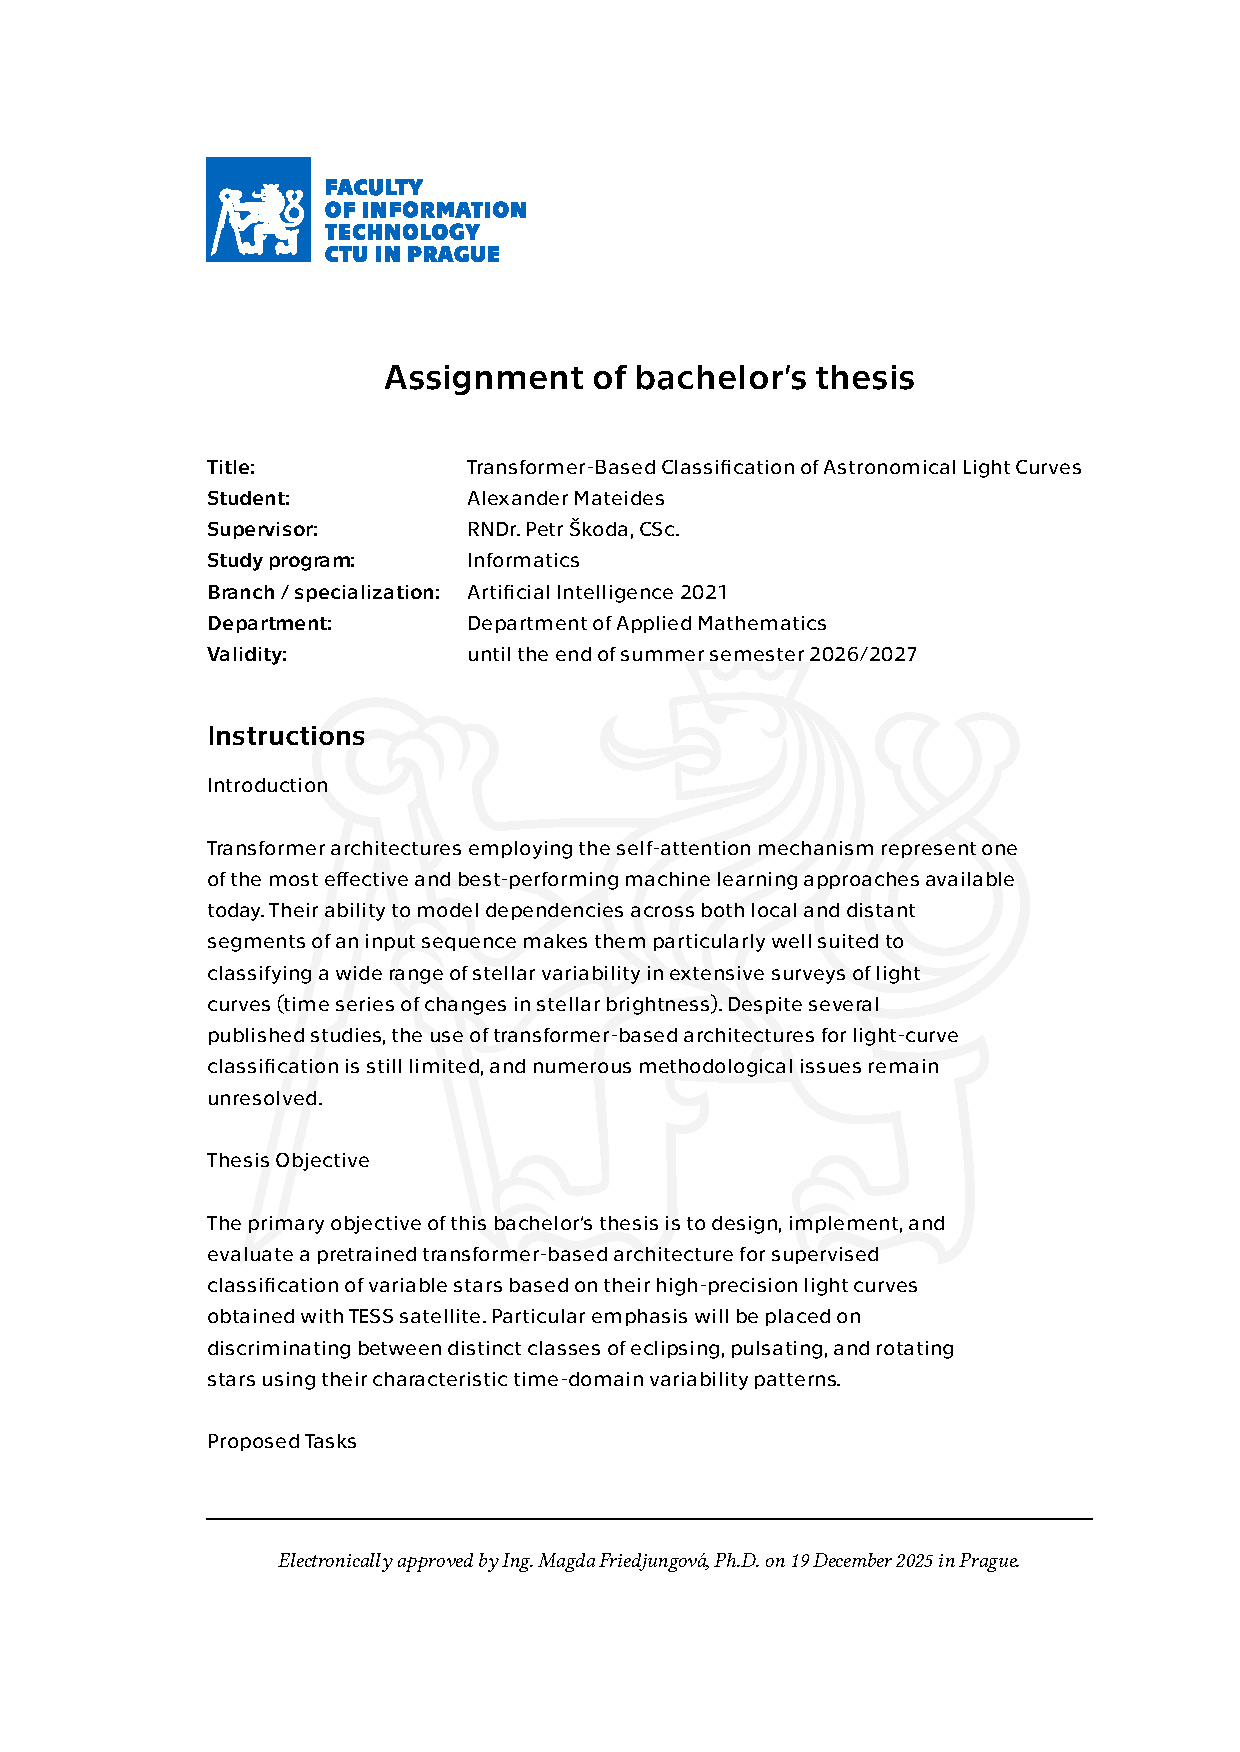
\includepdf[pages={1-}]{mateial1-assignment.pdf} % replace this file with your thesis assignment generated from ProjectsFIT

    \imprintpage % do not remove this command
    \stopTOCentries

%%%%%%%%%%%%%%%%%%%
% ACKNOWLEDGMENT
% FILL IN / MODIFY
% This is a place to thank people for helping you. It is common to thank your supervisor.
%%%%%%%%%%%%%%%%%%%
    \begin{acknowledgmentpage}

        Firstly, I would like to express my sincere gratitude to my thesis supervisor, RNDr.\,Petr Škoda,\,CSc., for his wise counsel, helpful recommendations and continuous support in the creation of this work.

        I would also like to thank Mgr.\,Marek Skarka\,Ph.D. for generously providing the light curve datasets used in this thesis and for his insightful comments regarding the classification of variable stars.

        My deepest thanks go to my parents for their continuous love and support throughout my journey in life that made it possible to reach this point.

        Furthermore, the access to the computational infrastructure of the OP VVV funded project CZ.02.1.01/0.0/0.0/16\_019/0000765 ``Research Center for Informatics'' is also gratefully acknowledged.
    \end{acknowledgmentpage}
%%%%%%%%%%%%%%%%%%%
% ACKNOWLEDGMENT END
%%%%%%%%%%%%%%%%%%%


%%%%%%%%%%%%%%%%%%%
% DECLARATION
% FILL IN / MODIFY
%%%%%%%%%%%%%%%%%%%
% INSTRUCTIONS
% ENG: choose one of approved texts of the declaration. DO NOT CREATE YOUR OWN. Find the approved texts at https://courses.fit.cvut.cz/SFE/download/index.html#_documents (document Declaration for FT in English)
% CZE/SLO: Vyberte jedno z fakultou schvalenych prohlaseni. NEVKLADEJTE VLASTNI TEXT. Schvalena prohlaseni najdete zde: https://courses.fit.cvut.cz/SZZ/dokumenty/index.html#_dokumenty (prohlášení do ZP)
    \begin{declarationpage}
        I hereby declare that the presented thesis is my own work and that I have cited all sources of
        information in accordance with the Guideline for adhering to ethical principles when elaborating an
        academic final thesis.

        I acknowledge that my thesis is subject to the rights and obligations stipulated by the Act No.
        121/2000 Coll., the Copyright Act, as amended. In accordance with Section 2373(2) of Act No.
        89/2012 Coll., the Civil Code, as amended, I hereby grant a non-exclusive authorization (licence) to
        utilize this thesis, including all computer programs that are part of it or attached to it and all
        documentation thereof (hereinafter collectively referred to as the "Work"), to any and all persons
        who wish to use the Work. Such persons are entitled to use the Work in any manner that does not
        diminish the value of the Work and for any purpose (including use for profit). This authorisation is
        unlimited in time, territory and quantity.

        I declare that I have used AI tools during the preparation and writing of my thesis. I have verified
        the generated content. I confirm that I am aware that I am fully responsible for the content of the
        thesis.
    \end{declarationpage}
%%%%%%%%%%%%%%%%%%%
% DECLARATION END
%%%%%%%%%%%%%%%%%%%

% Use one of the two following commands. The first prints abstracts+keywords on two pages, the second puts them on one page (if possible). \printonepageabstract can also accept optional argument that specifies a vertical space before both abstracts (the default is 18 mm).
    \printtwopageabstract
%\printonepageabstract

%%%%%%%%%%%%%%%%%%%
% SUMMARY
% FILL IN / MODIFY
% OR REMOVE ENTIRELY (upon agreement with your supervisor)
% (appropriate to remove in most theses)
%%%%%%%%%%%%%%%%%%%
% \begin{summarypage}
% \section*{Summary section}
%
% \lipsum[1][1-8]
%
% \section*{Summary section}
%
% \lipsum[2][1-6]
%
% \section*{Summary section}
%
% \lipsum[3]
%
% \section*{Summary section}
%
% \lipsum[2]
%
% \section*{Summary section}
%
% \lipsum[1][1-8] Lorem lorem lorem.
% \end{summarypage}
%%%%%%%%%%%%%%%%%%%
% SUMMARY END
%%%%%%%%%%%%%%%%%%%

    \tableofcontents % do not remove this command
%%%%%%%%%%%%%%%%%%%%%%
% list of other contents: figures, tables, code listings, algorithms, etc.
% add/remove commands accordingly
%%%%%%%%%%%%%%%%%%%%%%
    \listoffigures % list of figures
    \begingroup
    \let\clearpage\relax
    \listoftables % list of tables. Remove if you do not have any.
    \thectufitlistingscommand{} % list of code listings. Remove if you do not have any.
    \thectufitlistofalgorithmscommand{} % list of algorithm pseudocodes defined using the algorithm package.
    \endgroup
%%%%%%%%%%%%%%%%%%%%%%
% list of other contents END
%%%%%%%%%%%%%%%%%%%%%%

%%%%%%%%%%%%%%%%%%%
% ABBREVIATIONS
% FILL IN / MODIFY
% OR REMOVE ENTIRELY
% List the abbreviations in lexicography order.
%%%%%%%%%%%%%%%%%%%


    \chapter{\thectufitabbreviationlabel}

    \begin{tabular}{rl}
        LLM  & Large Language Model         \\
        SOTA & State-Of-The-Art             \\
        VT & Vision Transformer \\
        CNN  & Convolutional Neural Network \\
        TSFM & Time Series Foundation Model \\
        TESS & Transiting Exoplanet Survey Satellite \\
        EA & Algol-type eclipsing binary \\
        EB & Beta Lyrae-type eclipsing binary \\
        EW & W Ursae Majoris-type eclipsing binary \\
        DSCT & Delta Scuti pulsating variable \\
        GDOR & Gamma Doradus pulsating variable \\
        RRAB & RR Lyrae pulsating variable (type AB) \\
        RRAC & RR Lyrae pulsating variable (type C) \\
        ROTM & Magnetic rotator variable \\
        ROTS & Spotted rotator variable \\
        NLP & Natural Language Processing \\
        MLP & Multi-Layer Perceptron \\
        GLU & Gated Linear Unit \\
        FFN & Feed-Forward Network \\
        LoRA & Low Rank Adaptation \\
        QLoRA & Quantized Low Rank Adaptation \\
        HF   & HuggingFace                  \\
        PEFT & Parameter Efficient Fine-Tuning \\
        TP   & True Positive                \\
        FP   & False Positive               \\
        TN   & True Negative                \\
        FN   & False Negative               \\
        ECG  & Electrocardiogram            \\
        TPF & Target Pixel File \\
        TIC & TESS Input Catalog \\
        CLS (token) & Learnable classification token \\
        FFT & Fast Fourier Transform \\




    \end{tabular}
%%%%%%%%%%%%%%%%%%%
% ABBREVIATIONS END
%%%%%%%%%%%%%%%%%%%
    \resumeTOCentries
    \mainmatter\mainmatterinit % do not remove these two commands
%%%%%%%%%%%%%%%%%%%
% THE THESIS
% MODIFY ANYTHING BELOW THIS LINE
%%%%%%%%%%%%%%%%%%%

    % Do not forget to include Introduction
%---------------------------------------------------------------
\chapter{Introduction}
% uncomment the following line to create an unnumbered chapter
%\chapter*{Introduction}\addcontentsline{toc}{chapter}{Introduction}\markboth{Introduction}{Introduction}
%---------------------------------------------------------------
\setcounter{page}{1}

Variable stars play a fundamental role in advancing our understanding of the universe, particularly in cosmology and stellar physics.
Their study has contributed to numerous major scientific discoveries, such as the calculation of the rate of at which the universe expands. \parencite{Hubble1929}
In addition, the analysis of variable stars can support the detection of extraterrestrial planets which is one of the main areas of research at the Astronomical Institute of Czech Academy of Sciences.

Recent technological progress has led to substantial improvements in photometric instrumentation, enabling the development of large-scale astronomical surveys such as OGLE (Optical Gravitational Lensing Experiment --~\cite{Udalski2008}), the Kepler planet-detection mission \parencite{Borucki2010}, the Zwicky Transient Facility survey \parencite{Bellm2019}, and TESS (Transiting Exoplanet Survey Satellite --~\cite{Ricker2014}).
These surveys generate enormous volumes of high-quality astronomical data, including light curves.
However, the scale of these datasets makes manual classification of variable stars both time-consuming and impractical, creating a strong need for automated methods.

Machine learning approaches have proven to be an effective solution for automated classification, enabling researchers to process large amounts of data quickly and accurately.
Moreover, deep learning methods, such as CNNs, have often outperformed more traditional machine learning techniques, such as Random Forests and K-means clustering.

In recent years, transformer-based models have emerged as a promising alternative to earlier deep learning approaches in many domains, including time-series classification, where they often achieve very good performance.
Fine-tuning pretrained transformer models, such as LLMs, TSFMs and VTs, has also shown potential in a variety of tasks by leveraging the powerful pattern-recognition capabilities acquired during pretraining.

In this thesis, we investigate the viability of transformer-based models for light curve classification.
Although previous studies have already explored this topic, our goal is to provide a more comprehensive analysis by considering both transformers trained from scratch and fine-tuned large pretrained models.



 % include `text.tex' from `text/' subdirectory
    \chapter{Astronomical Background}

Light curves describe how the brightness of an astronomical object varies over time and therefore are a type of time series.
These brightness variations are caused by different astrophysical phenomena, such as pulsations, rotation and eclipses.

Since the underlying causes of variability are most often related to changes in physical properties of a star, understanding of these processes is crucial for interpretation, preprocessing and classification of light curves.
We therefore provide a brief introduction to the relevant astronomical and astrophysical terms, concepts and processes, more detailed general overview can be found in~\textcite{Guidry2019}.

\section{Stars}

\textbf{Stars} are luminous spherical celestial bodies composed primarily of plasma that are held together by their gravity.
They emit radiation due to their immense temperature, which can reach over $\num{30000} K$, this energy is primarily caused by thermonuclear fusion of elements in their cores. \parencite{Girichidis2020}

There are approximately $\num{9000}$ stars visible to the naked eye, the brightest of them have been categorized into stellar constellations and even given names long before the invention of the telescope.
With the use of modern astronomical instruments, hundreds of millions more stars have been discovered and indexed in star catalogues.
However, this is still only a tiny fraction of the estimated $10^{24}$ stars in the observable universe. \parencite{Traversa2021}

\subsection{Stellar Classification}

Stars are primarily classified based on their spectral characteristic and by extension their effective temperature and luminosity.

\begin{itemize}
    \item \textbf{Effective Temperature} is the temperature that a blackbody would have if it emitted the same amount of energy as electromagnetic radiation. \linebreak
    It is used as an approximation of surface temperature of the star.
    Additionally, effective temperature also influences the star's perceived color since it determines the shape of the emitted spectrum.
    \item \textbf{Luminosity} is a measure of electromagnetic energy that the star radiates per unit of time and is determined by the star's surface area and effective temperature.
\end{itemize}

\subsubsection{Harvard Classification System}

The \textbf{Harvard Classification System} \parencite{Cannon1918} categorizes stars based on spectral characteristics, assigning a letter to each class.
These classes are then subdivided by Arabic numerals 0--9 for finer classification.

\begin{table}[H]
    \centering
    \scriptsize
    \renewcommand{\arraystretch}{1.1}

    \begin{tabularx}{\textwidth}{X c c c}
        \toprule
        \textbf{Class} & \textbf{Temperature (K)} & \textbf{Apparent color} & \textbf{\% of main sequence stars} \tabularnewline
        \midrule
        \textbf{O} & $\geq \num{33000}$              & blue            & 0.00003 \tabularnewline
        \textbf{B} & 10 000--33 000     & bluish white    & \num{0.12}    \tabularnewline
        \textbf{A} & 7300--10000      & white           & \num{0.61}    \tabularnewline
        \textbf{F} & 6000--7300       & yellowish white & \num{3.00}    \tabularnewline
        \textbf{G} & 5300--6000       & yellow          & \num{7.60}     \tabularnewline
        \textbf{K} & 3900--5300       & orange          & \num{12.00}   \tabularnewline
        \textbf{M} & 2300--3900       & red             & \num{76.00}   \tabularnewline
        \bottomrule
    \end{tabularx}

    \caption[Harvard Classification System]{Harvard Classification System}
    \label{tab:02_harvard_classification}
\end{table}

\FloatBarrier

he Sun is classified as a \textbf{G2} star in the Harvard classification system.

\subsubsection{Morgan--Keenan System}

\textbf{Morgan--Keenan} (MK) classification \parencite{Morgan1973} system extends the Harvard system by introducing luminosity classes.

\begin{table}[H]
    \centering
    \scriptsize
    \renewcommand{\arraystretch}{1.1}
    \begin{tabularx}{\textwidth}{X c}
        \toprule
        \textbf{Luminosity Class} & \textbf{Description} \tabularnewline
        \midrule
        \textbf{Ia$^{+}$}  & Hypergiants \tabularnewline
        \textbf{Ia}        & Luminous supergiants \tabularnewline
        \textbf{Iab}       & Intermediate-luminous supergiants \tabularnewline
        \textbf{Ib}        & Less luminous supergiants \tabularnewline
        \textbf{II}        & Luminous giants \tabularnewline
        \textbf{III}       & Normal giants \tabularnewline
        \textbf{IV}        & Subgiants \tabularnewline
        \textbf{V}         & Main-sequence stars (dwarfs) \tabularnewline
        \textbf{VI (sd)}   & Subdwarfs \tabularnewline
        \textbf{VII (d)}   & White dwarfs \tabularnewline
        \bottomrule
    \end{tabularx}

    \caption[Morgan-Keenan Luminosity Classes]{Morgan-Keenan Luminosity Classes}
    \label{tab:02_ml_classification}
\end{table}

\FloatBarrier

\smallskip

\noindent Since the Sun is a main-sequence star, its luminosity class is \textbf{V}; therefore its designation in the MK system is \textbf{G2V}.

\subsection{Hertzsprung--Rusel Diagram}

\textbf{Hertzsprung--Russel Digram} (HR diagram) is a two-dimensional plot showing the relationship between stellar luminosities and effective temperatures. \linebreak
It is often used to either describe stellar distribution of some region (i.e.~a stellar cluster) or to illustrate a star's evolution in time.

\begin{figure}[!htbp]
    \centering
    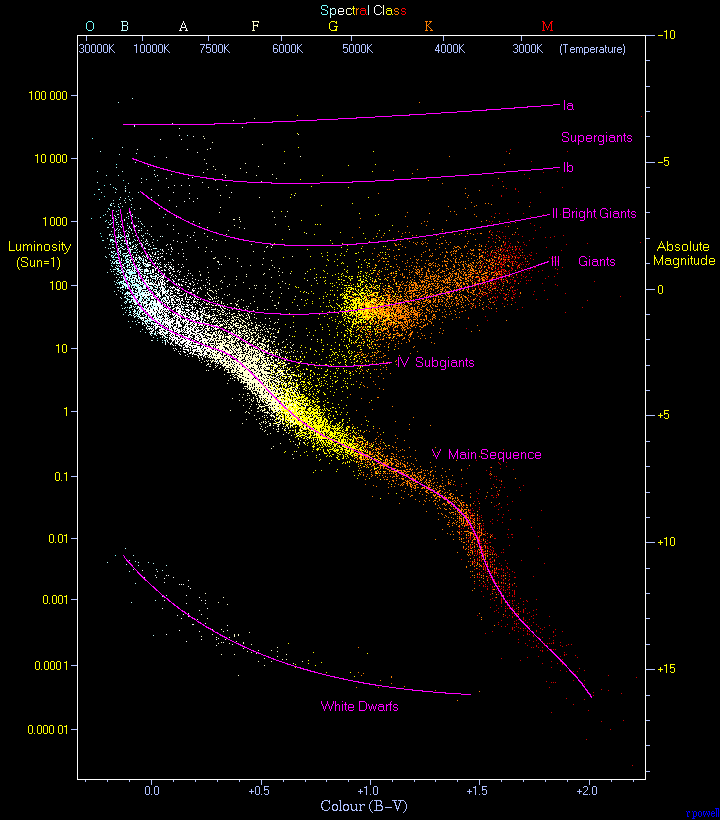
\includegraphics[width=0.8\linewidth]{images/02_hr_diagram}
    \caption[Hertzsprung--Russell diagram]{Hertzsprung--Rusell diagram with 22,000 stars plotted from the Hipparcos Catalogue and 1,000 from the Gliese Catalogue of nearby stars.It shows stars of different masses in different stages of their lifecycles. \parencite{hr_diagram}}
    \label{fig:02_hr_diagram}
\end{figure}

\FloatBarrier


\section{Stellar Evolution}

\textbf{Stellar Evolution} describes how stars are born, how they change over the course of their lives, and how they eventually die.
Knowledge of these processes is vital for understanding many types of variable stars, since their variability is often associated with instabilities in stars at later stages of their lifecycle. \parencite{Aguirre2017}

\subsection{Formation}

Stars begin to form when clouds of gas, composed primarily of hydrogen and helium, gather under their own gravity.
As the collapsing material becomes denser and hotter, conditions eventually become sufficient for thermonuclear fusion to start.
The initial mass of the star influences its type, lifecycle and ultimately its eventual fate. \parencite{Girichidis2020}

\subsection{Main Sequence}

After formation, the star spends most of its lifetime on the main sequence, fusing hydrogen into helium in its core.
As helium slowly accumulates in the core during the main sequence, the core contracts and heats up and fusion accelerates, which in turn makes the star burn hotter and brighter. \parencite{Schonberg1942}

The duration of the main sequence primarily depends on how quickly the star burns its hydrogen fuel.
Generally, more massive stars have greater pressures and temperatures in their cores, which leads to significantly higher rates of fusion.
As a result, they have much shorter lifespans and are more luminous. \parencite{Schonberg1942}

The Sun's total main sequence duration is expected to be around $10$ billion years, of which around $4.6$ billion already passed.
In comparison, the duration of main sequence for massive stars is in the order of millions of years whereas the least massive stars are expect to last for trillions of years. \parencite{Laughlin1997}

\subsection{Post-main sequence}

\subsubsection{Low-mass Stars}

\textbf{Low-mass Stars} with masses $\lesssim 0.5 \, M_{\odot}$ are generally massive enough to start helium fusion.

These stars evolve very slowly, therefore their post-main sequence hasn't been observed yet.
Since less massive of these stars are small enough for their entirety to be a convection zone, an electron-degenerate\footnote{Quantum-mechanical phenomenon that occurs when the gas particles are packed so tightly (due to gravity) that the electrons are forced to occupy all available quantum states, exerting pressure. This allows the helium core to accumulate heat without expanding and cooling down like a normal gas.} helium core cannot form and the star will continue to burn hydrogen until it turns almost all of it into helium.
Once the supply of hydrogen is exhausted, they won't have enough temperature to start helium fusion and will slowly turn into helium white dwarfs.

Stars at the upper end of this mass range may become red giants, but their cores won't reach the required temperatures for helium fusion, they too will end as white dwarfs. \parencite{Nelson1986}

\subsubsection{Intermediate-mass Stars}

\textbf{Intermediate-sized Stars}, with masses of roughly 0.5--8 $M_{\odot}$, are massive enough to eventually start helium fusion but generally not massive enough to sustain advanced fusion of heavier elements. \parencite{Aguirre2017}

\begin{figure}[!htbp]
    \centering
    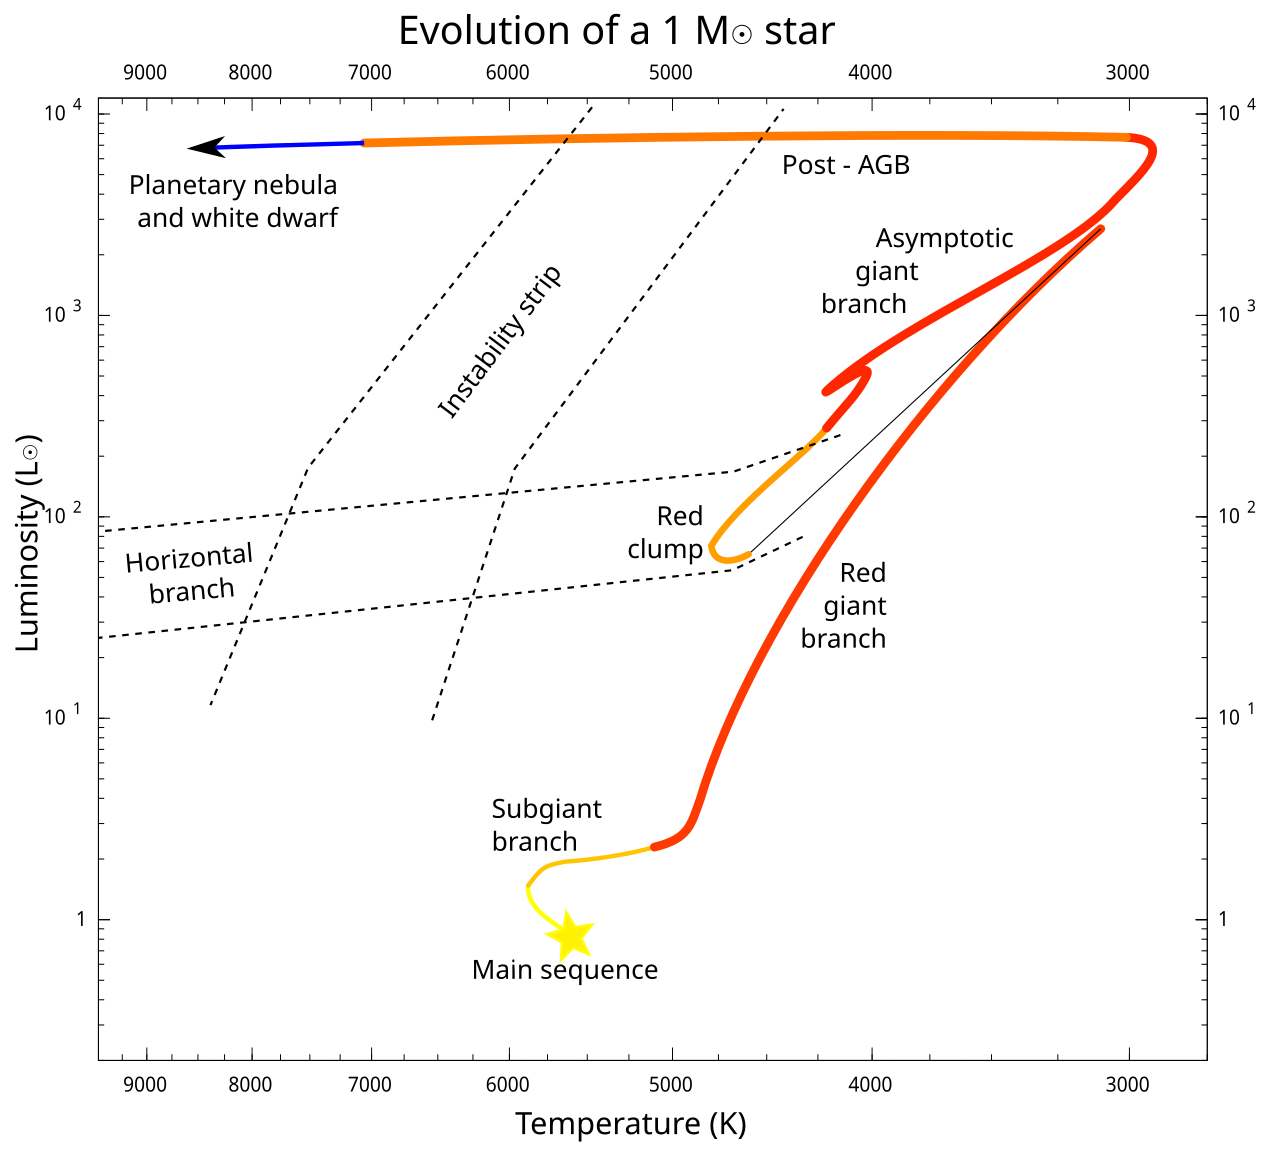
\includegraphics[width=0.475\linewidth]{images/02_stellar_evolution}
    \hfill
    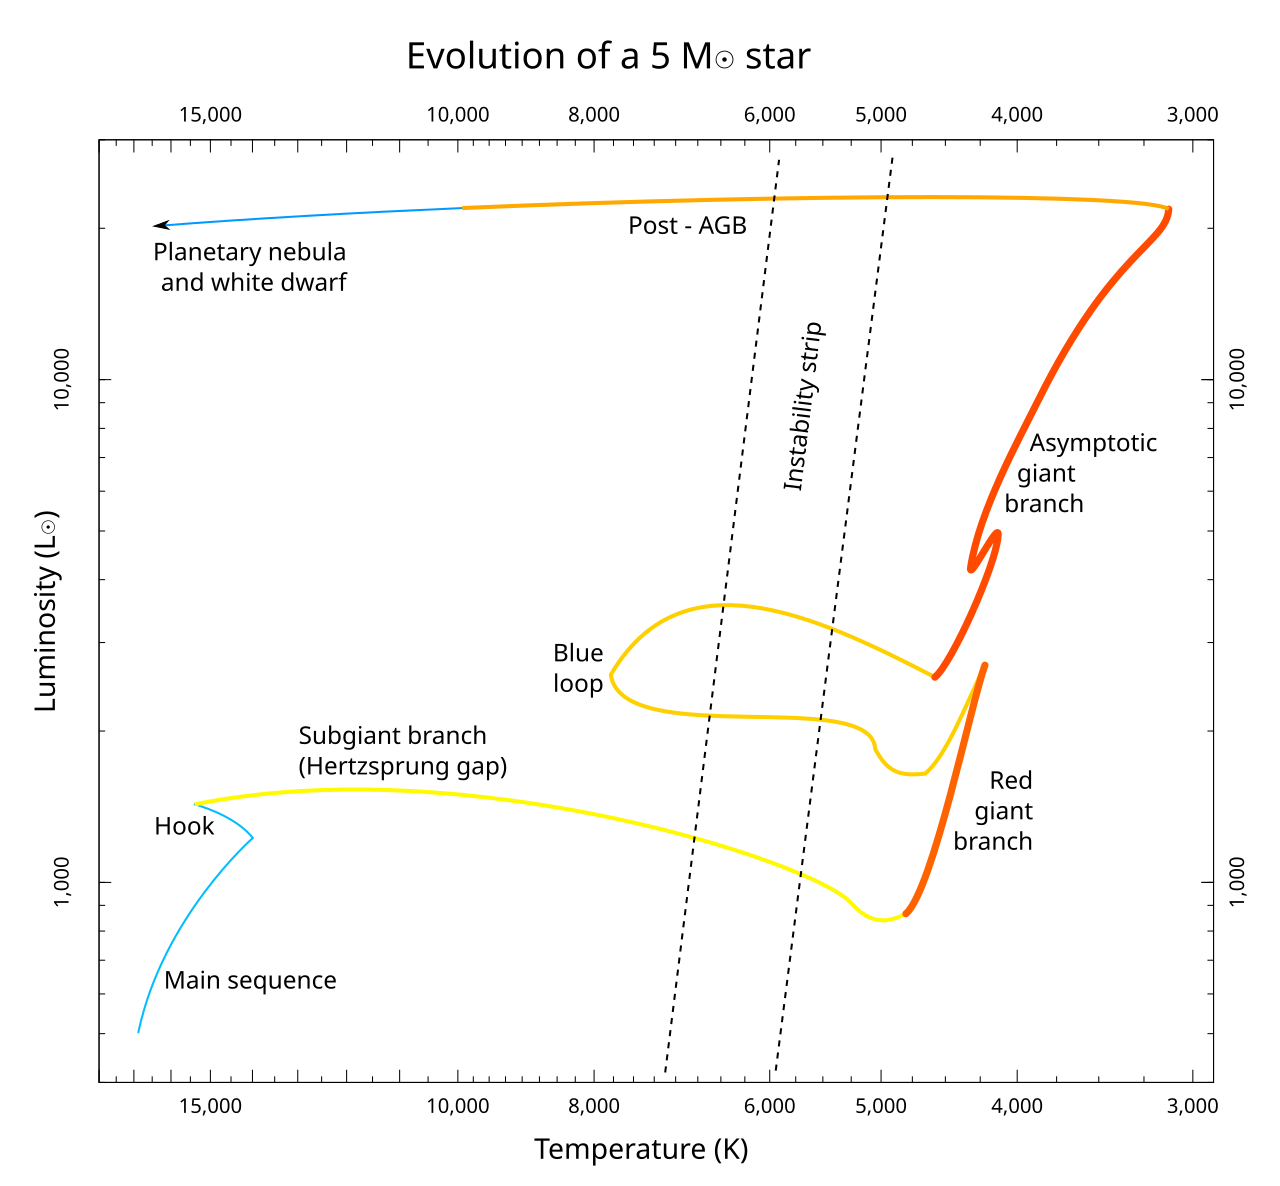
\includegraphics[width=0.485\linewidth]{images/02_stellar_evolution2}
    \caption[Stellar Evolution diagrams]{Two HR diagrams showing slightly different evolution of two intermediate-sized stars. \parencite{hr_diagram_1m_star, hr_diagram_5m_star}}
    \label{fig:02_stellar_evolution}
\end{figure}

\begin{enumerate}
    \item \textbf{Subgiant Phase.}  As stars fuse all the hydrogen in their cores into helium, they leave the main sequence and continue burning hydrogen in a shell around an inert helium core.
    As more helium is produced in the shell, the core slowly increases in mass, this leads to core degeneracy and contraction in less massive stars (around $1 \, M_{\odot}$) or natural increase in core temperature in more massive stars. \parencite{Renzini1981}

    \item \textbf{Red Giant Branch Phase.} The contracting helium core heats up, increasing the temperature of the hydrogen-burning shell around it, which accelerates fusion.
    The rising temperature creates pressure that causes the outer layers of the star to expand enormously, creating a red giant with a large radius and relatively cool surface.
    Although the surface is relatively cold, red giants are highly luminous due to their size. \parencite{Aguirre2017}

    \item\label{item:02-horiozntal-branch}\textbf{Horizontal Branch.} Eventually, the core heats up enough to start helium fusion.
    In less massive stars ($m \lesssim 2.3 \, M_{\odot}$) core degeneration allows the accumulation of thermal energy in the core, which leads to the rapid start of helium fusion in an event known as the helium flash.

    More massive stars with non-degenerate cores are able to start the helium fusion more smoothly and due to their larger mass, they become even hotter in this stage, performing a so-called blue loop. \parencite{Renzini1981}

    \item \textbf{Asymptotic Giant Branch (AGB).} As most of the helium in the core is fused into carbon, the star expands and cools down, increasing its luminosity and becoming a red giant again.
    This stage is characterized by an inert carbon and oxygen core, an inner shell where helium fusion happens and an outer shell where hydrogen is being fused.

    Eventually, the fusion in the helium shell stops being stable as the star slowly depletes its fuel and decreases its temperature.
    The star then gets its energy only from the fusion of hydrogen in its outer shell.

    Periodically, enough helium accumulates, igniting the shell explosively in a brief thermal pulse.
    These periodical vents extremely increase the star's luminosity for a short time and allow heavier elements from the core to mix with outer layers.

    The emissions of material caused by thermal pulses and solar wind then surrounds the AGB star with a circumstellar envelope enriched with heavier elements from the core. \parencite{Renzini1981}

    \item \textbf{Post-AGB Phase.} The star eventually ceases all hydrogen and helium fusion and sheds its outer layers, allowing the core to contract and heat up.

    The shedding of outer layers combined with the previous emissions of material form a protoplanetary nebula around the contracting core.
    As the core shrinks and heats up, the emitted radiation ionizes the surrounding nebula forming a planetary nebula with a hot central star.

    Finally, the planetary nebula disperses, leaving only the central star, now called a white dwarf. \parencite{Renzini1981}
\end{enumerate}

\begin{figure}[!htbp]
    \centering
    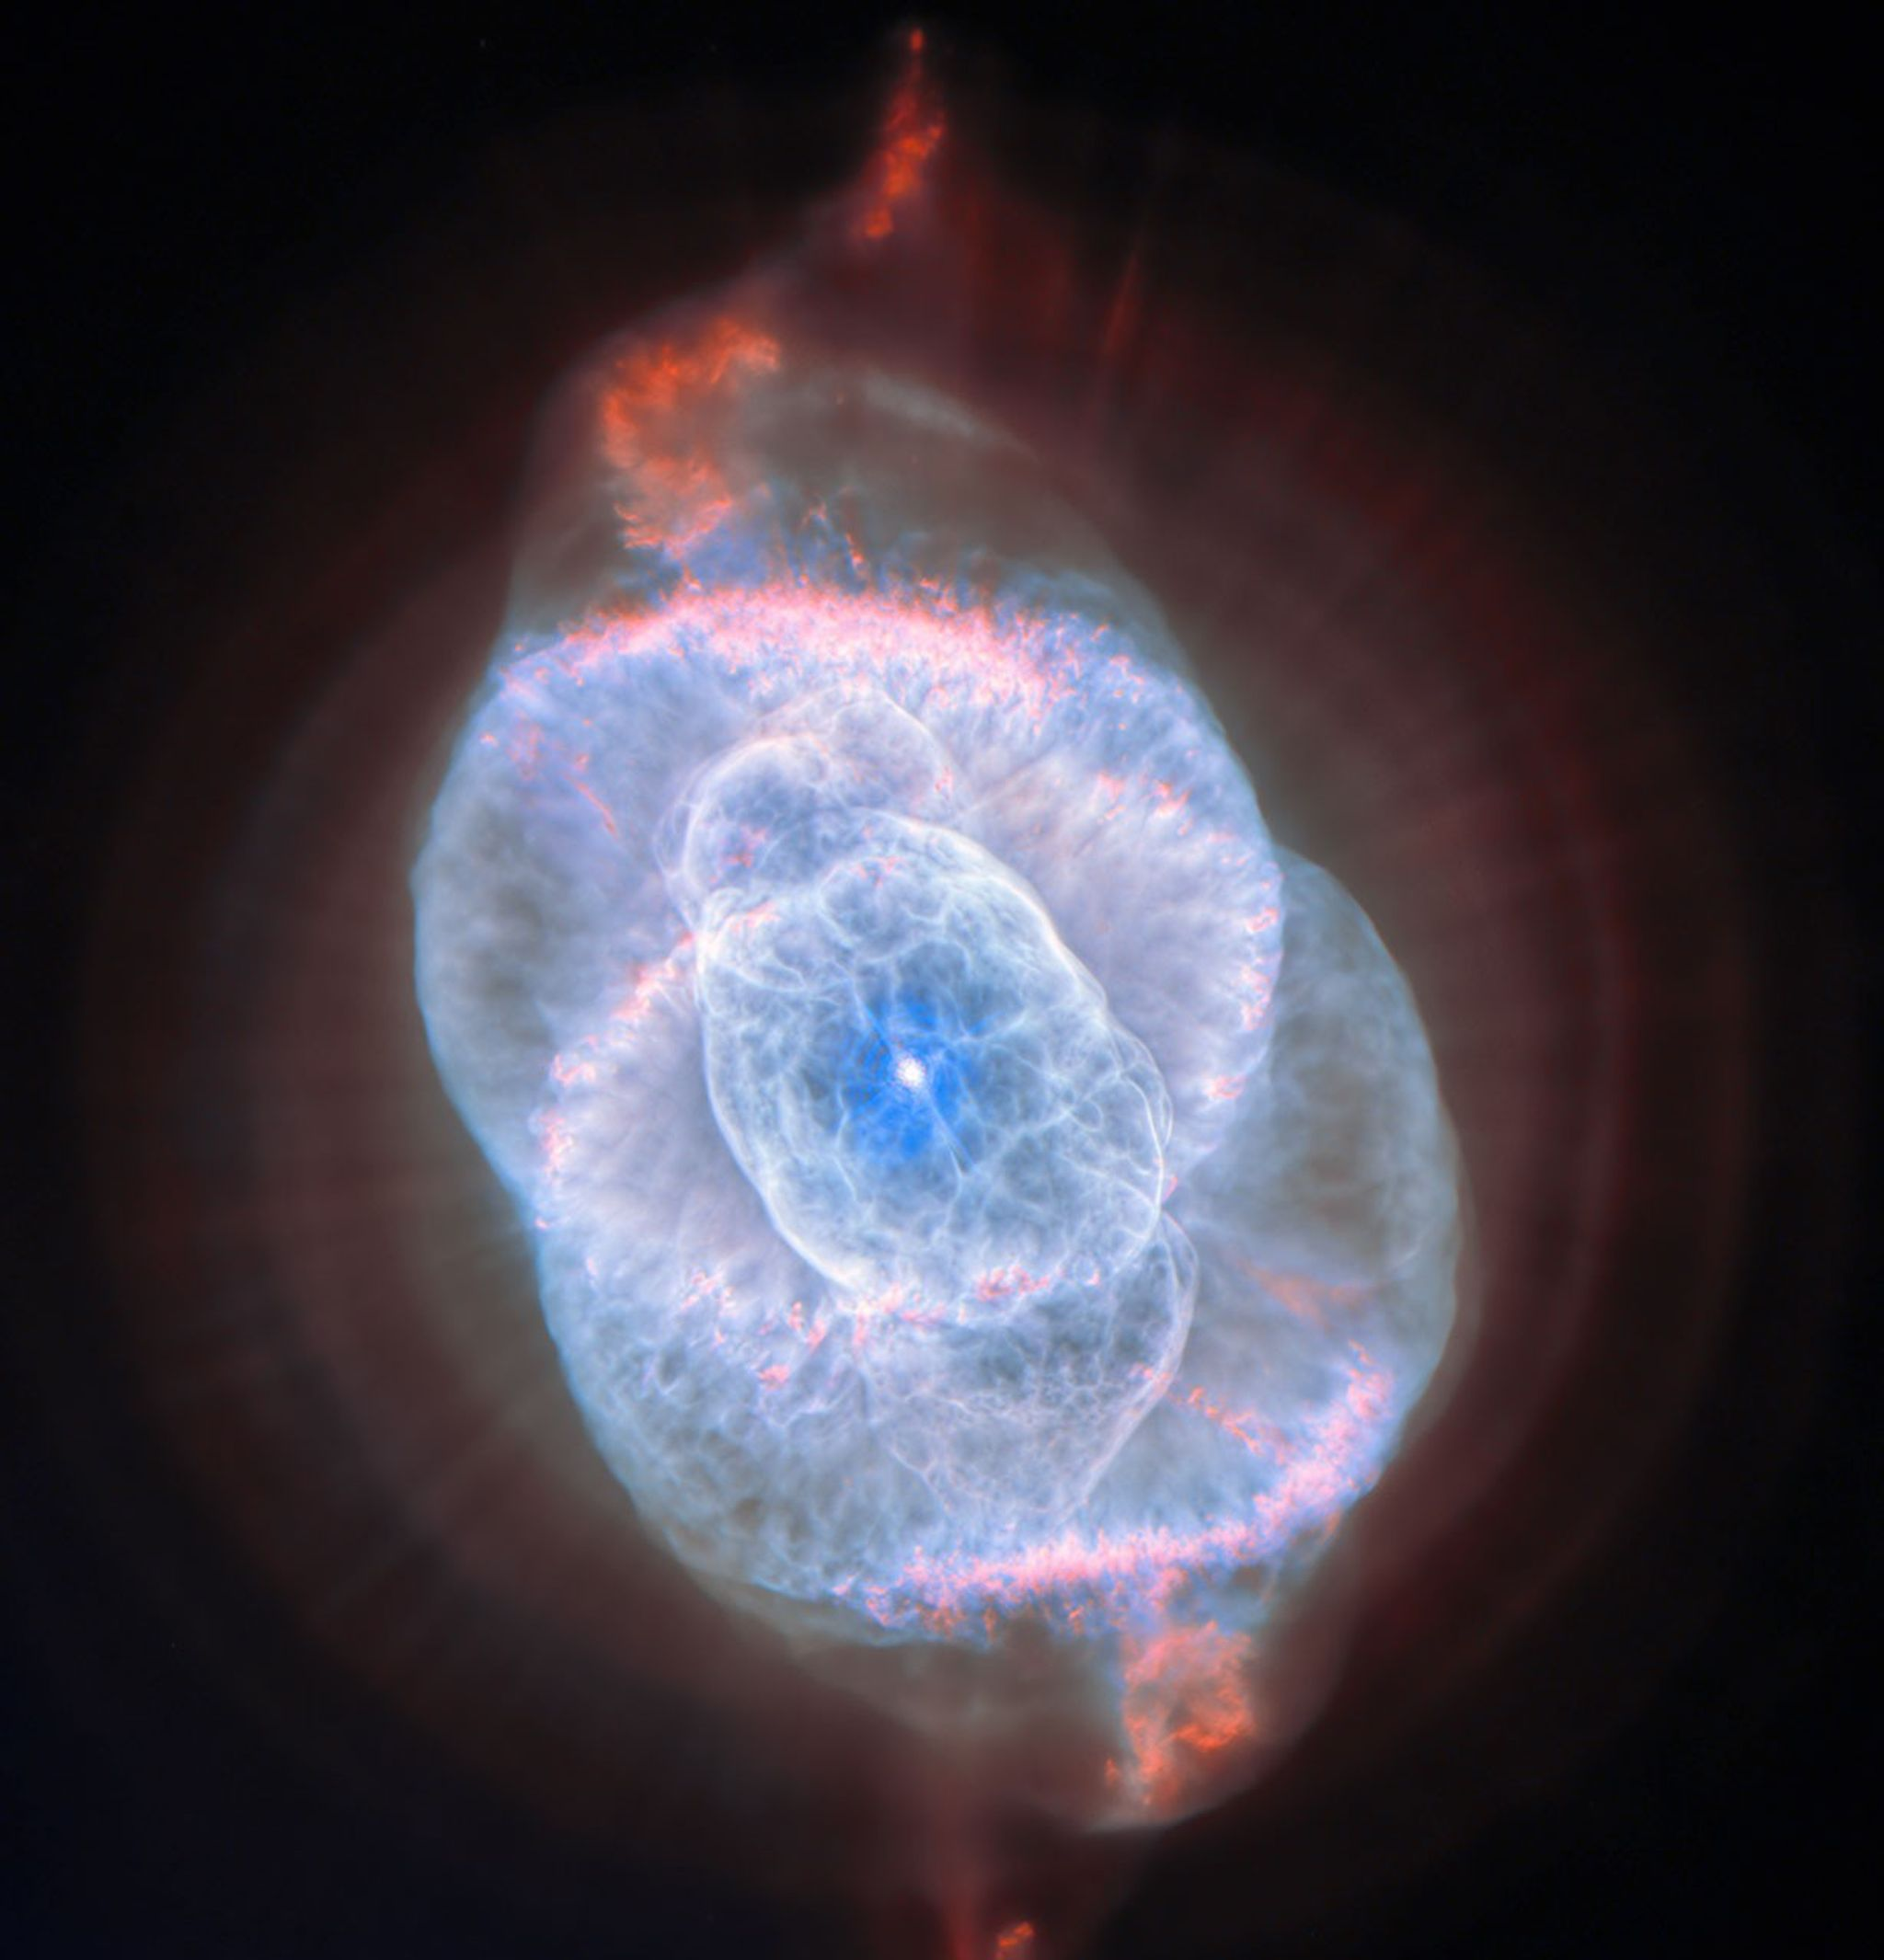
\includegraphics[width=0.6\linewidth]{images/02_planetary_nebula}
    \caption[Cat's Eye planetary nebula]{Cat's Eye planetary nebula captured with the Hubble telescope. \parencite{planetary_nebula}}
    \label{fig:02_planetary_nebula}
\end{figure}

\FloatBarrier

\subsubsection{Massive Stars}

\textbf{Massive Stars}  with masses $\gtrsim 8 \, M_{\odot}$ can reach high enough temperatures to start the fusion of carbon and subsequently heavier elements like neon, oxygen and silicon in their giant phase.

The stages of fusion get exponentially shorter with the last stage where silicon fuses into iron-group\footnote{Iron, Cobalt and Nickel} elements lasting mere days.
Since iron-group nuclei lie around the peak of nuclear binding energy, their fusion no longer releases any energy.
Once an iron core forms, the fusion stops and the core collapses under its own gravity in seconds. \parencite{Woosley2002}

The collapse of the core releases immense amounts of energy, resulting in a supernova.
During the explosion, much of the stellar envelope is ejected into the surrounding space, forming a nebula.
The remnants of the collapsed core will, depending on the original mass, form either a neutron star or a black hole.
In rare cases of supermassive stars, the supernova obliterates the entire core so no remnant is left. \parencite{Woosley2002}

\FloatBarrier


\section{Light Curves}

A \textbf{Light Curve} is a plot of a star's brightness as a function of time and is a crucial tool for studying stars, especially variable ones.
In practice, observations are often limited to a specific wavelength range.
In real datasets, light curves often contain gaps, caused by factors such as daylight, weather conditions or observing cadence.

Light curves can be either aperiodic (i.e.~supernovae) or periodic (i.e.~eclipsing binaries).

\begin{figure}[!htbp]
    \centering
    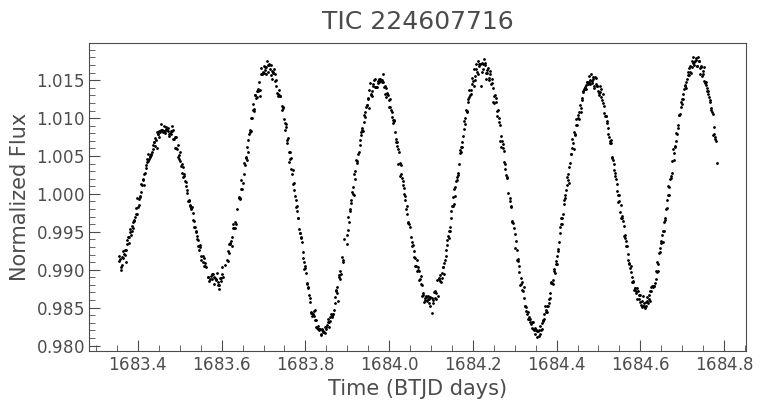
\includegraphics[width=0.6\linewidth]{images/02_light_curve}
    \caption[Light Curve]{Light curve of a magnetic rotator (ROTM) star, the variability is caused by spots on the surface that fade in and out of view due to rotation.}
    \label{fig:02_light_curve}
\end{figure}

\FloatBarrier


\subsection{Apparent Magnitude}

\textbf{Apparent Magnitude} ($m$) is a measure of a star's brightness as seen from the Earth.
It depends on the star's intrinsic luminosity, its distance from the observer and any obstructions in the line of sight, such as interstellar dust or eclipses.

The scale is reverse logarithmic with a ratio of $\sqrt[5]{100}$ - a magnitude 1.0 star is $~2.512$ times brighter than a magnitude 2.0 star and $100$ times brighter than a magnitude 6 star.

\subsection{Periodogram}\label{subsec:02-periodogram}

Periodicity in light curves is usually analyzed using Fourier-based methods \parencite{Das2021} or the Lomb--Scargle periodogram \parencite{Lomb1976, Scargle1983}, the latter being often preferred due to better performance on unevenly sampled data.
A periodogram is then constructed to show the dominant periods or frequencies in the analyzed signal.

Additionally, many stars show multiple periodicities and/or their periods change during their lifetime, therefore additional care must be taken in later preprocessing steps.

\begin{figure}[!htbp]
    \centering
    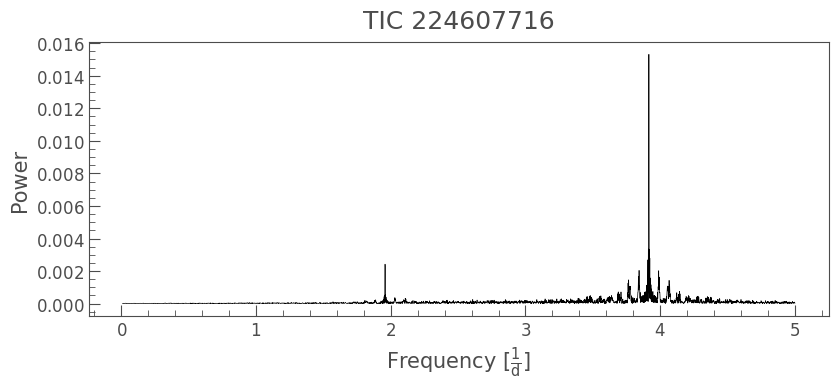
\includegraphics[width=0.6\linewidth]{images/02_periodogram}
    \caption[Light Curve]{Periodogram of a ROTM star showing its rotation period of around $0.25$ day.}
    \label{fig:02_periodogram}
\end{figure}

\FloatBarrier


\subsection{Phase-folded Light Curve}\label{subsec:02-phase-folded-light-curve}

Once a suitable period has been identified, the light curve can be phase-folded.
Phase folding maps the time axis onto phase by taking the observation times modulo the selected period, causing repeated cycles to overlap.
The folded data are then binned and aggregated, for example by taking the mean of each bin, in order to reduce noise and obtain a smoother representation.

Phase-folding is an important preprocessing step for machine learning applications, because it transforms time component into a dimensionless phase, allowing a unified data format across an entire dataset of various different light curves.

\begin{figure}[!htbp]
    \centering
    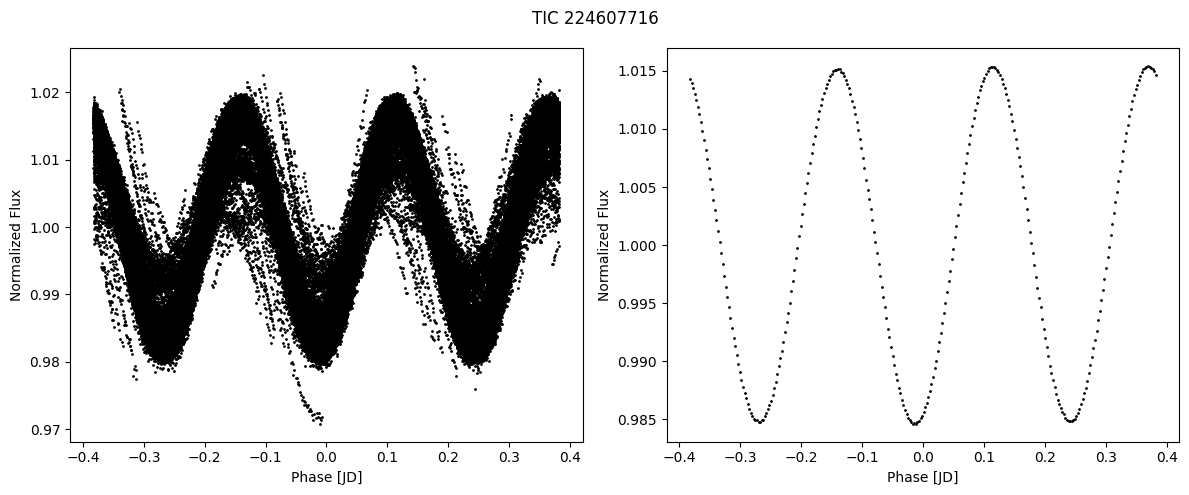
\includegraphics[width=0.95\linewidth]{images/02_phase_folded_lc}
    \caption[Phase-folded Light Curve]{Phase-folded light curve and its binned counterpart of a ROTM star.}
    \label{fig:02_phase_folded_light_curve}
\end{figure}

\FloatBarrier



\section{Variable Stars}\label{sec:02-variable-stars}

\textbf{Variable Stars} are stars whose observed brightness changes over time.
This variation in brightness can happen due to multiple different causes. \parencite{Percy2007}
Variable stars are commonly classified according to the origin of their variability as:

\begin{itemize}
    \item \textbf{Intrinsic variables} - variability is caused by an inherent change in luminosity, such as stellar pulsation.
    \item \textbf{Extrinsic variables} - variability is caused by a change in the amount of light that can reach Earth, such as eclipses or starspots.
\end{itemize}

The changes in brightness occur on vastly different time scales between different stars, ranging from minutes to several years.
While most stars exhibit some signs of variability, the relative change in the amount of emitted light varies from star to star.
For example, the Sun exhibits variations of about $0.1\%$ over its 11-year cycle, whereas some stars can exhibit variations greater than one magnitude.

Some stars display multiple different types of variability simultaneously which can complicate classification.
In addition, contamination from nearby light sources can also distort the observations. \parencite{Percy2007}

\subsection{Eclipsing Binary Variables}

\textbf{Eclipsing Binary Variables} are binary stars which orbit a common center of gravity and their orbit is positioned to the Earth in such a way, that one star can block light of the second one, causing a dip in the system's brightness. \parencite{Kopal1946}

In most cases, the stars differ in brightness; the brighter star is then called primary and the dimmer one secondary.
In that case, two different brightness dips can be observed:

\begin{itemize}
    \item \textbf{Primary eclipse.} The brighter star is eclipsed, resulting in a deeper minimum.
    \item \textbf{Secondary eclipse.} The dimmer stars is eclipsed, resulting in a shallower minimum.
\end{itemize}

We then distinguish three main subtypes of eclipsing binary systems.

\subsubsection{Algol-type (EA)}

\textbf{Algol-type (EA)} variables, also referred to as detached binaries, are systems where the two stars are widely separated, so that the luminosity of the entire system is mostly unchanged, except for their eclipse.
Their light curves are therefore characterized by relatively sharp and well-defined eclipses. \parencite{Kopal1946}

\begin{figure}[!htbp]
    \centering
    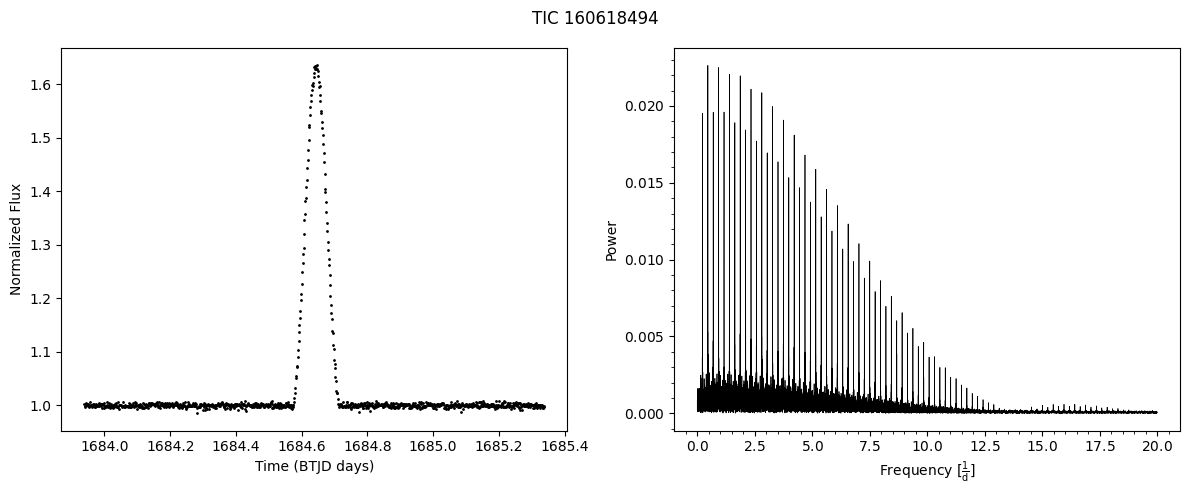
\includegraphics[width=0.95\linewidth]{images/02_ea}
    \caption[EA Variable]{Light curve and periodogram of a typical EA Variable.}
    \label{fig:02_ea_variable}
\end{figure}

\FloatBarrier


\subsubsection{Beta Lyrae-type (EB)}

\textbf{Beta Lyrae-type (EB)} variables, also referred to as semi-detached binaries, are binary stars that orbit so close together that their shapes becomes distorted.
Material flow from one star to another is usually present, because one of the stars fills its Roche lobe\footnote{Region around a star within which the material is gravitationally bound to that star.}.

The variation period is very regular, lasting 1--10 days in most cases.
Because of the distorted stellar shapes and ongoing mass transfer, the variation is more continuous and the eclipses are not as sharply defines as in EA systems. \parencite{Kopal1946}

\begin{figure}[!htbp]
    \centering
    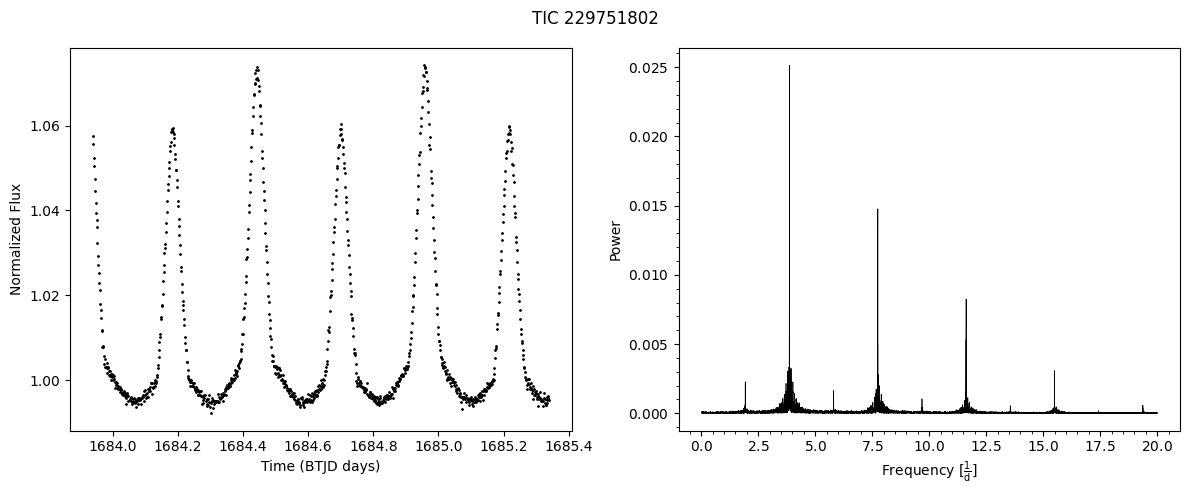
\includegraphics[width=0.95\linewidth]{images/02_eb}
    \caption[EB Variable]{Light curve and periodogram of a typical EB Variable.}
    \label{fig:02_eb_variable}
\end{figure}


\subsubsection{W Ursae Majoris-type (EW)}

\textbf{W Ursae Majoris-type (EW)} variables, also referred to as contact binaries, are binaries that are so close together that they share a common envelope, allowing material to flow between them.

Their orbital periods are usually shorter than one day and their range of magnitude is typically lower than in the case of detached systems.
Furthermore, since they continuously distort each other via gravity, their light curves undergo additional variation. \parencite{Kopal1946}

\begin{figure}[!htbp]
    \centering
    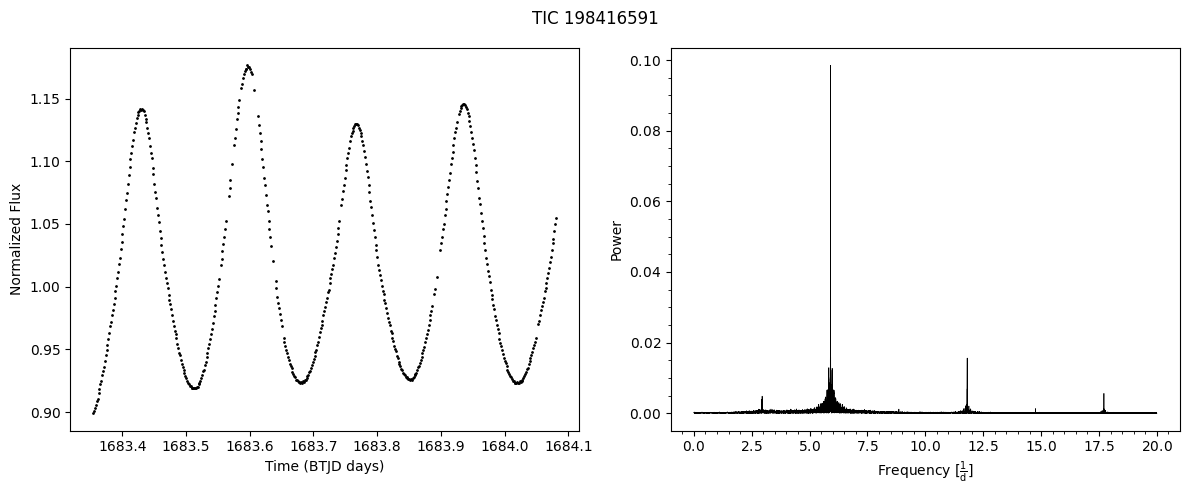
\includegraphics[width=0.95\linewidth]{images/02_ew}
    \caption[EW Variable]{Light curve and periodogram of a typical EW Variable.}
    \label{fig:02_ew_variable}
\end{figure}

\FloatBarrier


\subsection{Pulsating Variables}

The variability in pulsating stars (pulsators) is caused by periodic expansion and contraction of their outer layers, which directly influences the star's luminosity. \parencite{Percy2007}

Stellar pulsation is commonly divided into two types:

\begin{itemize}
    \item \textbf{Radial.} The star expands uniformly, maintaining a spherical shape.
    \item \textbf{Non-radial.} The star expands asymmetrically and becomes non-spherical.
\end{itemize}

\subsubsection{Cepheids}

\textbf{Cepheid} variables pulsate radially with relatively stable periods and amplitudes.
Their pulsations are driven by $\kappa\mathrm{-mechanism}$, which causes the star's opacity increase with temperature, increasing its luminosity. \parencite{Percy2007}


Additionally, they're divided into two main subclasses:

\begin{itemize}
    \item \textbf{Classical Cepheids.} Younger stars with very regular periods in the order of days to months.
    They are yellow bright giants and supergiants of classes F6-K2 with masses of 3--10 $M_{\odot}$.
    \item \textbf{Type II Cepheids.} Older stars with shorter periods (order of days), they are usually fainter and have lower mass (0.5--0.6 $M_{\odot}$).
\end{itemize}

\subsubsection{Delta Scuti (DSCT)}\label{subsubsec:02-dsct}

\textbf{Delta Scuti (DSCT)} variables are a type of pulsators similar to cepheids.
They are smaller main-sequence (or near main-sequence) stars of spectral classes A--F and are therefore considerably dimmer than cepheids, their range of magnitude also being lower.

Delta Scuti stars often show both radial and non-radial pulsations and their periods are shorter, ranging from minutes to several hours.
Furthermore, Delta Scuti variables often pulsate in multiple frequencies, making their light curves more complex. \parencite{Guzik2021}

\begin{figure}[!htbp]
    \centering
    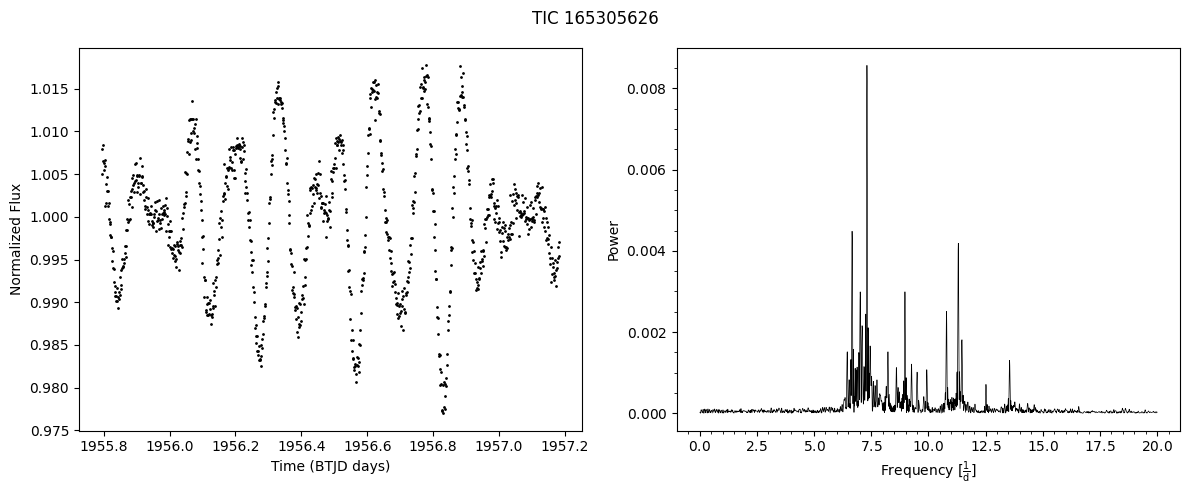
\includegraphics[width=0.95\linewidth]{images/02_dsct}
    \caption[DSCT Variable]{Light curve and periodogram of a typical DSCT Variable.}
    \label{fig:02_dsct_variable}
\end{figure}

\FloatBarrier


\subsubsection{Gamma Doradus (GDOR)}

\textbf{Gamma Doradus (GDOR)} variables pulsate mainly in non-radial gravity modes.
Like Delta Scuti variables, they're also A-F stars on the main sequence or slightly more evolved.
However, they pulsate mainly in gravity modes and have longer periods, ranging from hours to days.
Their range of magnitude is also typically lower. \parencite{Pollard2009}

\begin{figure}[!htbp]
    \centering
    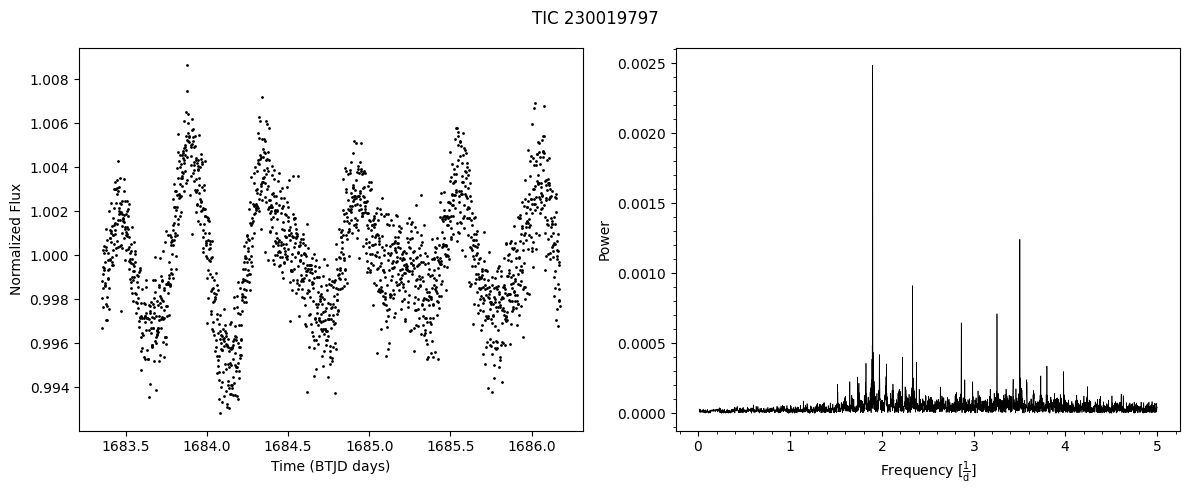
\includegraphics[width=0.95\linewidth]{images/02_gdor}
    \caption[GDOR Variable]{Light curve and periodogram of a typical GDOR Variable.}
    \label{fig:02_gdor_variable}
\end{figure}

\FloatBarrier



\subsubsection{RR Lyrae (RRAB / RRC)}

\textbf{RR Lyrae (RRAB / RRC)} variables are old stars on the horizontal branch of spectral classes A-F with masses around $0.5 \, M_{\odot}$.
They have similar range of magnitude and period duration to Cepheids, but are typically less stable and dimmer. \parencite{Marconi2009}

\begin{figure}[!htbp]
    \centering
    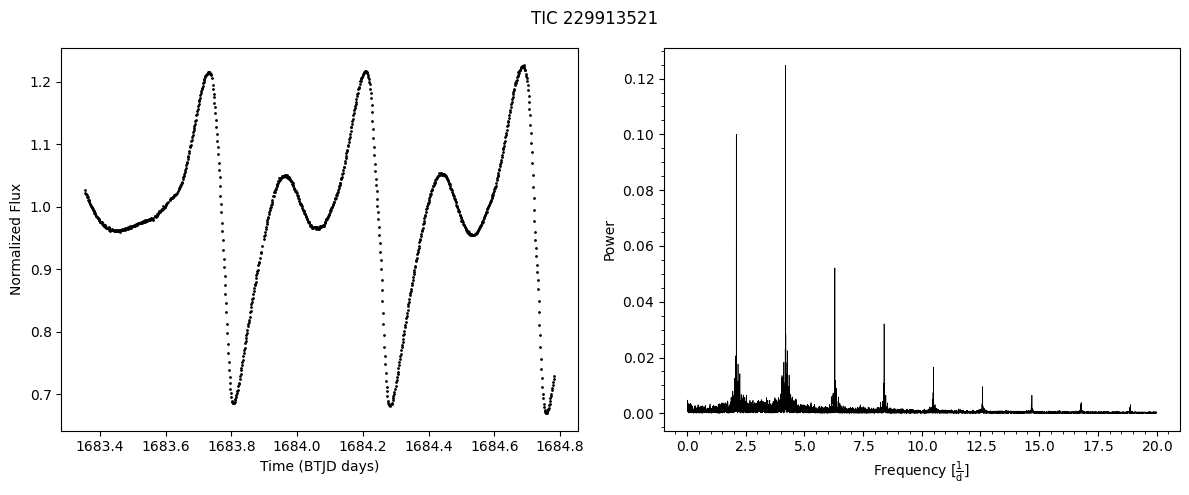
\includegraphics[width=0.95\linewidth]{images/02_rrab}
    \caption[RRAB Variable]{Light curve and periodogram of a typical RRAB Variable.}
    \label{fig:02_rrab_variable}
\end{figure}

\FloatBarrier


\subsection{Rotating Variables}

The variability in rotating stars is caused by the different luminosity of its uneven surface that is carried in and out of view by rotation.
Their periods are stable, given by the star's rotation period and typically range from hours to tens of days.
Magnitude range is usually low, a few tenths of a magnitude at the upper end. \parencite{Percy2007}

\subsubsection{Magnetic Rotators (ROTM)}\label{subsubsec:02_rotm}

\textbf{Magnetic Rotators (ROTM)} have spots mainly due to different element concentrations due to magnetic activity.
Their spots are relatively stable due to the magnetic field which makes their light curves consistent over time. \parencite{Percy2007}

\begin{figure}[!htbp]
    \centering
    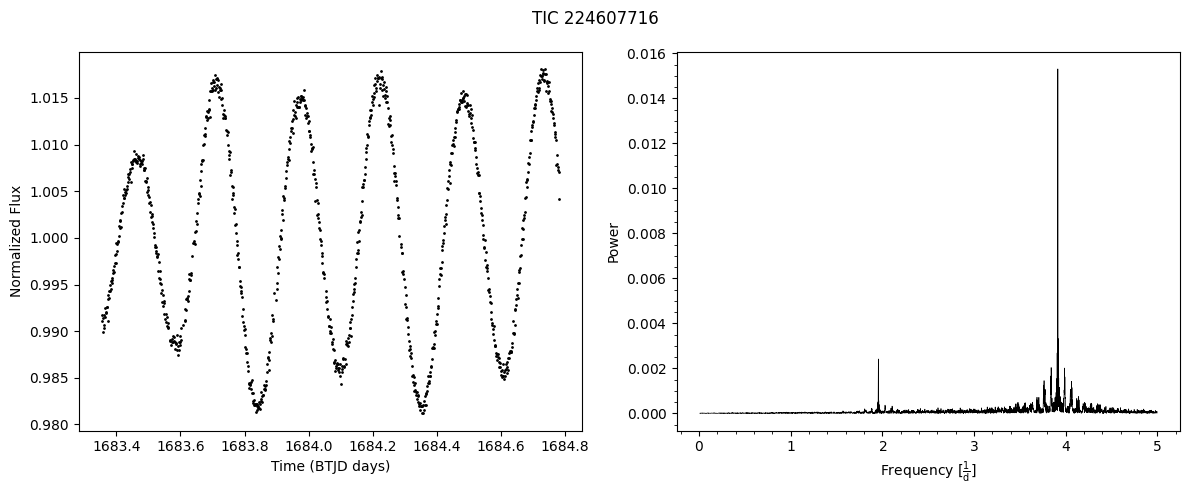
\includegraphics[width=0.95\linewidth]{images/02_rotm}
    \caption[ROTM Variable]{Light curve and periodogram of a typical ROTM Variable.}
    \label{fig:02_rotm_variable}
\end{figure}

\FloatBarrier


\subsubsection{Spotted Rotators (ROTS)}

\textbf{Spotted Rotators (ROTS)} have spots mainly due to surface regions with different temperatures that is often caused by irregular convection.
Their spots usually evolve over time, making their light curves more irregular than those of magnetic rotators. \parencite{Percy2007}

\begin{figure}[!htbp]
    \centering
    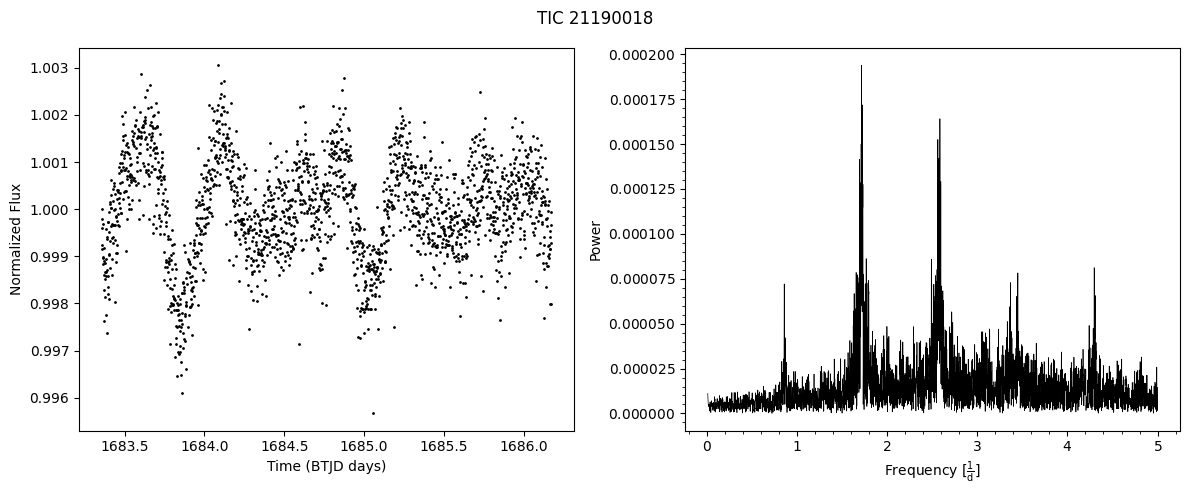
\includegraphics[width=0.95\linewidth]{images/02_rots}
    \caption[ROTM Variable]{Light curve and periodogram of a typical ROTS Variable.}
    \label{fig:02_rots_variable}
\end{figure}

\FloatBarrier




    \chapter{Overview of Technologies}

We provide a brief theoretical overview of the technologies used in this work and other important related methods that preceded them.
Additionally, a summary of the relevant libraries and frameworks used for the implementation of the experiments is also provided.


\section{Transformers}

\textbf{Transformers} \parencite{AttentionIsAllYouNeed} are a modern type of neural network architecture that has achieved remarkable results in various machine learning tasks, particularly in natural language processing (NLP), computer vision and sequence modeling, often outperforming previous SOTA solutions.
While the original transformer architecture was designed for NLP tasks, it has since been adapted and extended to a wide range of applications, including time series classification - the focus of this work.

While~\cite{AttentionIsAllYouNeed} introduce both encoder and decoder blocks in their work, for our task of time-series classification mainly the encoder blocks are relevant.

\subsection{High level workflow}

At a high level, a transformer processes an input sequence through the following steps:

\begin{enumerate}
    \item \textbf{Tokenize the input.}
    Split the input into a sequence of $n$ tokens.

    \item \textbf{Embed the tokens.}
    Map each token to a vector in the model's representation space, optionally adding positional information so the model can distinguish token order:
    \[
        X_0 \in \mathbb{R}^{n \times d_{\mathrm{model}}}.
    \]

    \item \textbf{Apply $L$ transformer layers.}
    For each layer $l = 1, \dots, L$, the model updates the token representations using attention and a feed-forward network:
    \begin{enumerate}
        \item \textbf{Multi-head self-attention.}
        Each token attends to other tokens in the sequence, producing context-aware representations:
        \[
            H_l = \mathrm{Attention}_l(X_{l-1}),
            \qquad
            H_l \in \mathbb{R}^{n \times d_{\mathrm{model}}}.
        \]

        \item \textbf{Residual connection and layer normalization.}
        The attention output is added back to the layer input, then normalized:
        \[
            U_l = \mathrm{LayerNorm}(X_{l-1} + H_l),
            \qquad
            U_l \in \mathbb{R}^{n \times d_{\mathrm{model}}}.
        \]

        \item \textbf{Feed-forward network (FFN).}
        A position-wise feed-forward network further transforms each token representation:
        \[
            F_l = \mathrm{FFN}_l(U_l),
            \qquad
            F_l \in \mathbb{R}^{n \times d_{\mathrm{model}}}.
        \]

        \item \textbf{Second residual connection and layer normalization.}
        The FFN output is added back to its input and normalized again:
        \[
            X_l = \mathrm{LayerNorm}(U_l + F_l),
            \qquad
            X_l \in \mathbb{R}^{n \times d_{\mathrm{model}}}.
        \]
    \end{enumerate}

    \item \textbf{Obtain final contextualized representations.}
    After the final layer, the model produces
    \[
        X_L \in \mathbb{R}^{n \times d_{\mathrm{model}}},
    \]
    where each token representation now encodes information about both the token itself and its surrounding context.

    \item \textbf{Generate task-specific outputs.}
    The final representations are mapped to outputs depending on the task:
    \begin{enumerate}
        \item \textbf{Sequence classification:}
        Select or pool one representation from $X_L$ (for example, a designated classification token), then apply a linear layer and softmax to produce class probabilities.

        \item \textbf{Next-token prediction:}
        Project each token representation in $X_L$ to vocabulary logits
        \[
            Z \in \mathbb{R}^{n \times |\mathcal{V}|},
        \]
        then apply softmax to obtain a probability distribution over the next token.
    \end{enumerate}
\end{enumerate}

\begin{figure}[!htbp]
    \centering
    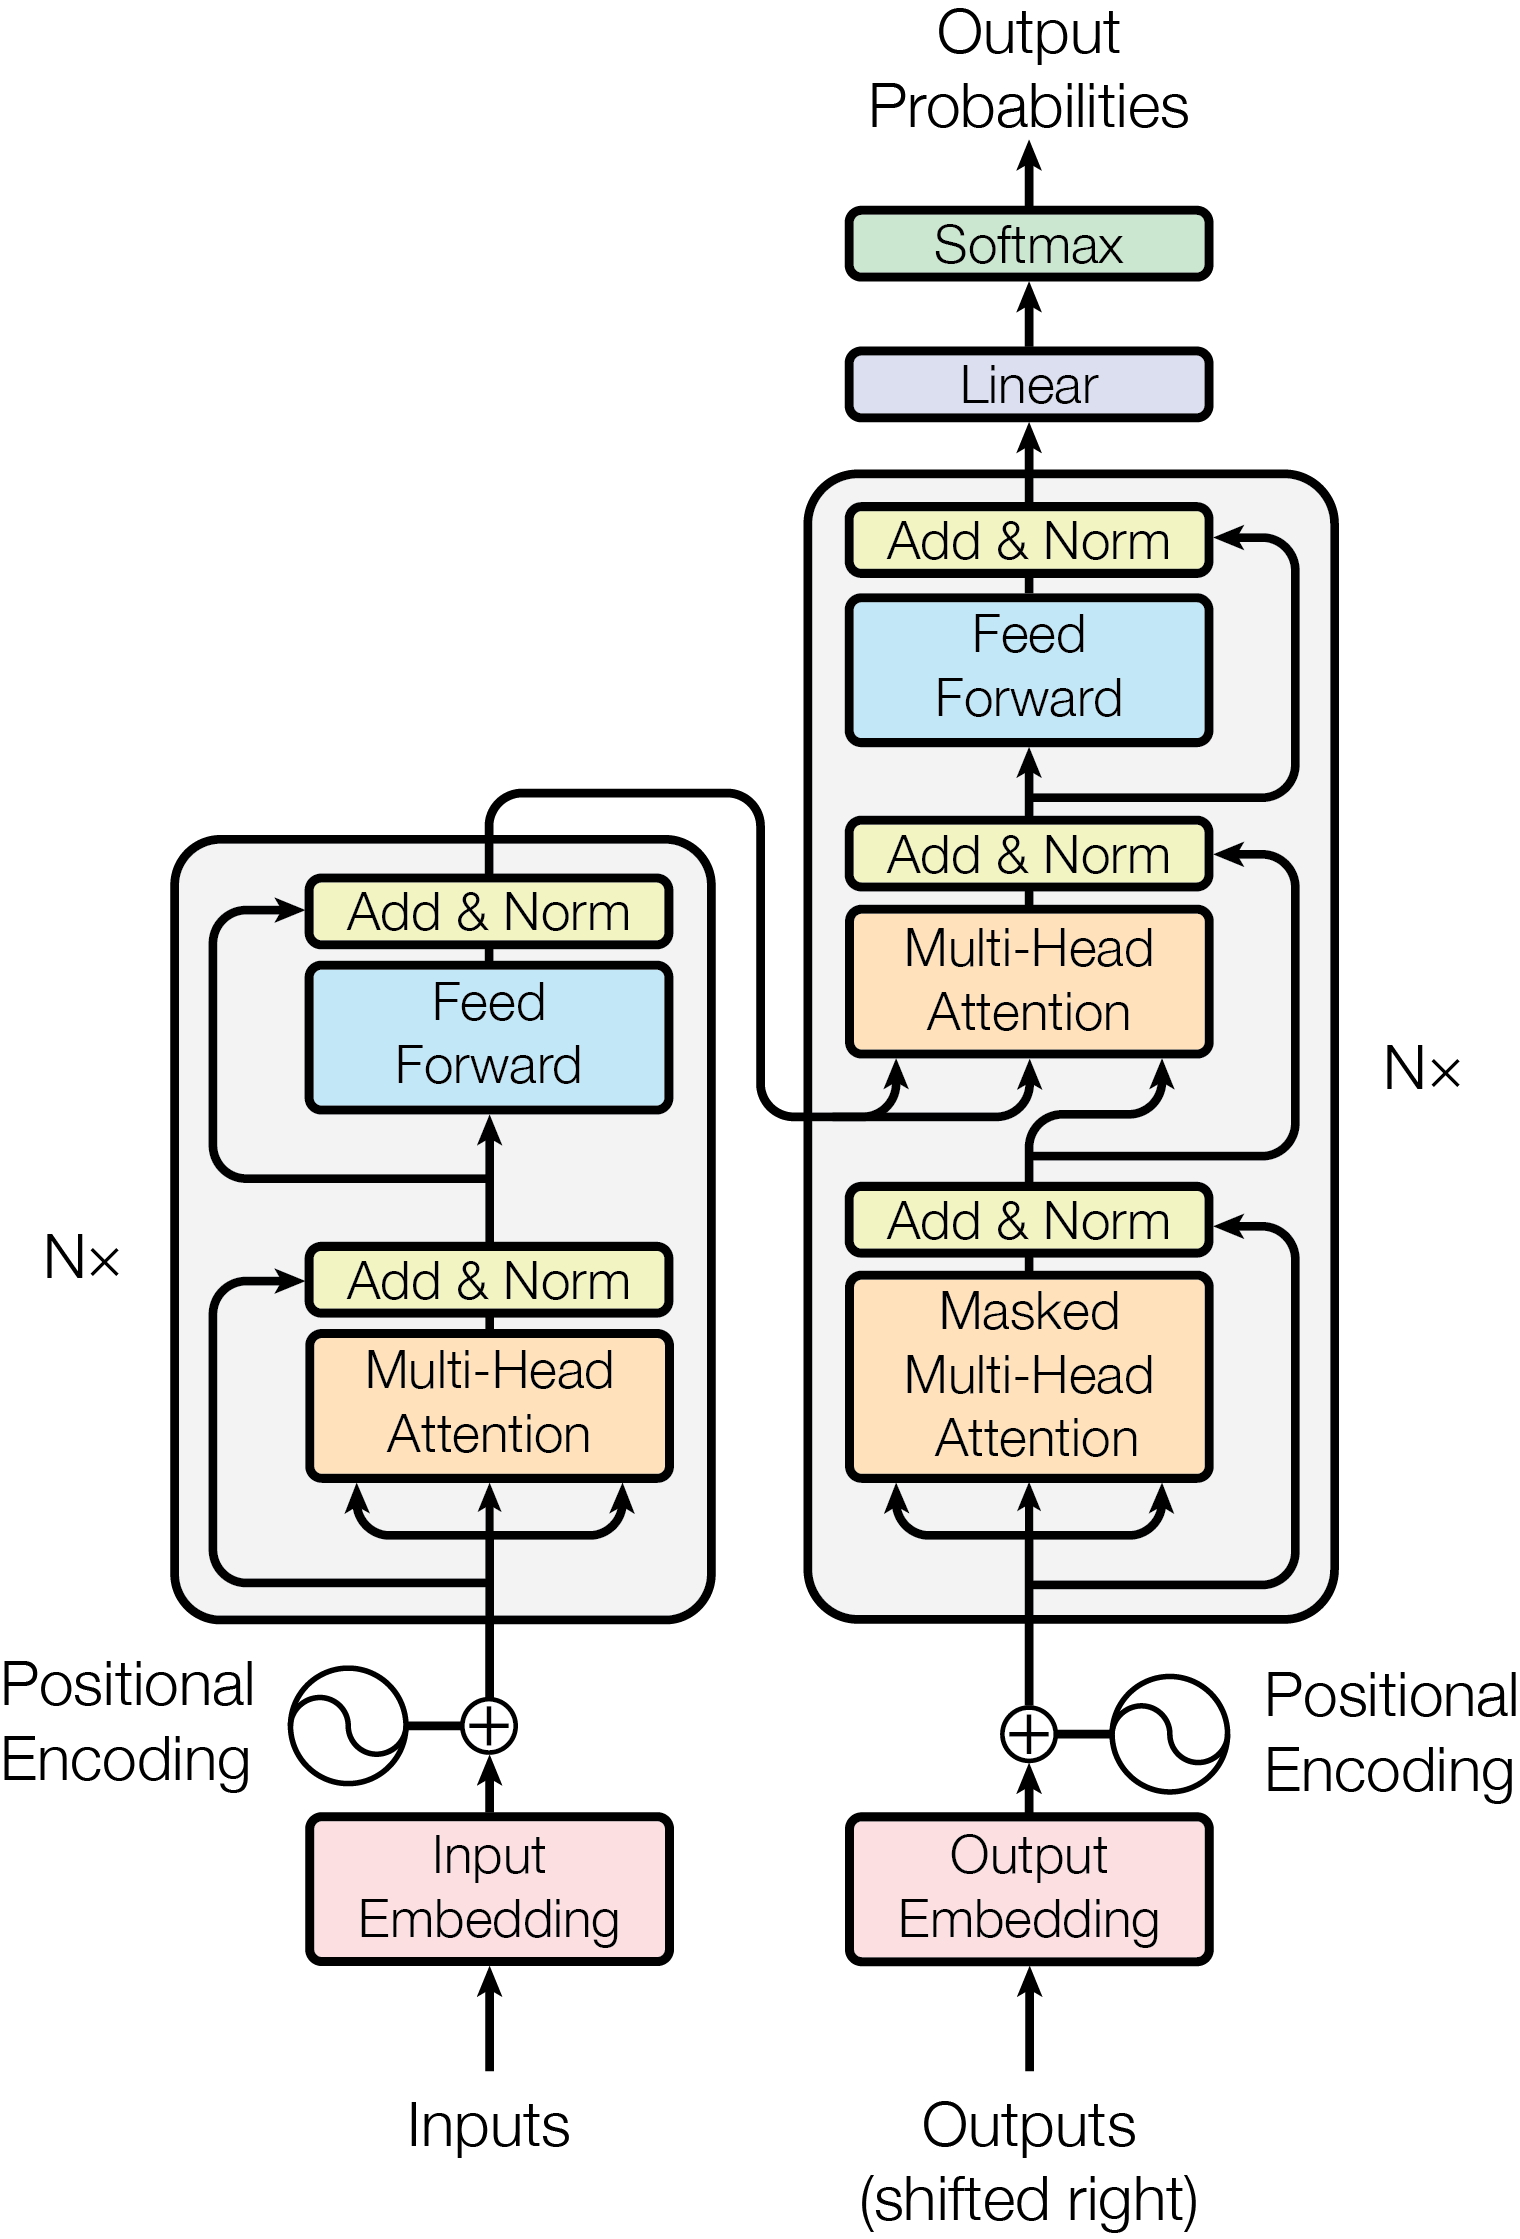
\includegraphics[width=\linewidth]{images/03_transformer}
    \caption[Transformer architecture]{Transformer architecture \parencite{AttentionIsAllYouNeed}}
    \label{fig:03_transformer}
\end{figure}

\subsection{Input and multimodality}

Historically, LLMs were primarily designed for NLP tasks, but recent advancements have led to the development of \textbf{multimodal models} that can process and generate data across multiple modalities, such as text, images and audio.

At its core, a multimodal model extends the transformer architecture to handle different kinds of input data by utilizing modality-specific encoders and decoders, as well as cross-modal attention mechanisms.

For our use-case of time-series classification, we can treat the data as a 1D input of dimension $d_{\mathrm{in}}$ and implement a custom \textbf{tokenizer} and \textbf{embedding layer}.

\subsubsection{Tokenizer}

\textbf{Tokenizer} is responsible for converting the raw data into a sequence of $n$ tokens of dimension $d_{\mathrm{token}}$ that can be processed by the embedding layer.

\subsubsection{Embedding Layer}

\textbf{Embedding Layer} projects the tokens into the model's representation space of dimension $d_{\mathrm{model}}$.

In the case of a fixed vocabulary of size $\mathcal{V}$ (i.e.\ LLMs), a parameter matrix $W \in \mathbb{R}^{\mathcal{V} \times d_{\mathrm{model}}}$ is learned during the training.
This allows the embedding layer to learn unique embedding for each token independently.

When the input is more diverse (i.e.\ time series) a learnable embedding layer is added instead.
Since this approach uses a linear projection it requires the tokens to be vectors of the same dimension $d_{\mathrm{token}}$.

\subsubsection{Positional Embeddings}

\textbf{Positional Embeddings} inject positional information into the embedding vector, allowing the transformer to distinguish token order during \textbf{Self-Attention}.

Two kinds of positional embeddings are commonly used

\begin{itemize}
    \item \textbf{Learned positional embeddings}: a parameter matrix $P \in \mathbb{R}^{L_{\mathrm{max}} \times d_{\mathrm{model}}}$ is learned during training.
    Each row of $P$ then corresponds to a different position in a sequence limited to length $L_{\mathrm{max}}$.
    \item \textbf{Sinusoidal positional embeddings} \parencite{AttentionIsAllYouNeed}: For position $p$ and dimension $i$
    \begin{align*}
        PE(pos, 2i) = \mathrm{sin} \left(\frac{p}{10000^{2i / d_{\mathrm{model}}}}\right) \\
        PE(pos, 2i + 1) = \mathrm{cos} \left(\frac{p}{10000^{2i / d_{\mathrm{model}}}}\right)
    \end{align*}
\end{itemize}

\subsection{Self-Attention Mechanism}

\textbf{Self-Attention} is an essential mechanism that allows the transformer model to add contextual information from the whole sequence to the evaluated token\footnote{Tokens are the elementary blocks of the input sequence (i.e. words)}.
This allows all tokens to influence the meaning of each other token, regardless of their distance in the sequence itself.
This is especially useful when long-range relationships in the data are important.

\bigskip

\noindent For a layer $l$, given weight matrices $W_Q, \, W_K, \, W_V \in \mathbb{R}^{d_{\mathrm{model}} \times (h d_{\mathrm{head}})}$ and a layer input $X_{l-1}$, the multi-head attention self-attention $H_l$ is calculated the following way

        {\setlength{\jot}{1em}
\begin{enumerate}
    \item \textbf{Compute $Q$ (queries), $K$ (keys), $V$ (values)} for each head $i \in \{1, 2, \dots, h\}$
    \[
        Q_i = X_{l-1}W^{(i)}_Q,
        \qquad
        K_i = X_{l-1}W^{(i)}_K,
        \qquad
        V_i = X_{l-1}W^{(i)}_V,
    \]
    $W_Q^{(i)}, \, W_K^{(i)}, \, W_V^{(i)} \in \mathbb{R}^{d_{\mathrm{model}} \times d_{\mathrm{head}}}$ are the weight matrices for the head $i$ and $Q_i, \, K_i, \, V_i \in \mathbb{R}^{n \times d_{\mathrm{head}}}$.
    \item \textbf{Compute attention scores $S_i$ for each head $i$}
    \[
        S_i = \frac{Q_{i}K_{i}^{\top}}{\sqrt{d_{\mathrm{head}}}},
        \qquad S_i \in \mathbb{R}^{n \times n},
    \]
    Each entry of $S_i$ then measures how strongly a token attends to another.
    \item \textbf{Apply row-wise softmax} to obtain \textbf{Attention weights}
    \[
        A_i = \mathrm{softmax}(S_i),
        \qquad
        A_i \in \mathbb{R}^{n \times n}.
    \]
    Each row of $A_i$ then sums to 1.
    \item \textbf{Compute weighted sum of the value vectors}
    \[
        Z_i = A_i V_i,
        \qquad
        Z_i \in \mathbb{R}^{n \times d_{\mathrm{head}}},
    \]
    This gives a context-aware representation based on all tokens in the sequence.
    \item \textbf{Concatenate the weighted sums} $Z_i$ of all $h$ heads
    \[
        Z = \mathrm{Concatenate}(Z_1, Z_2, \dots, Z_h),
        \qquad
        Z \in \mathbb{R}^{n \times (h d_{\mathrm{head}})},
    \]
    In most implementations $h d_{\mathrm{head}} = d_{\mathrm{model}}$.
    \item \textbf{Project back to model dimension} (output projection)
    \[
        H_l = ZW_O,
        \qquad
        H_l \in \mathbb{R}^{n \times d_{\mathrm{model}}},
    \]
    $W_O \in \mathbb{R}^{(h d_{\mathrm{head}}) \times d_{\mathrm{model}}}$ is the output projection weight matrix.

\end{enumerate}
}

\subsection{Feed-Forward Network (FFN)}

\textbf{Feed-Forward Network} is the second main component of a transformer layer which independently transforms each token after attention mixes information between tokens.
It usually consists of a two-layer MLP which projects the token vector into some higher dimensional hidden space of dimension $d_{\mathrm{ff}}$ and then back into the model space of dimension $d_{\mathrm{model}}$. \parencite{AttentionIsAllYouNeed}

This projection, combined with an activation function $\phi$\footnote{ReLU and GELU are commonly used activation functions in FFNs} gives the model additional capacity to express nonlinear combinations of features.
It has been shown that the mixing of feature information in FFN translates to the transformer's ability to learn complex patterns in the data. \parencite{Dai2022}
\bigskip

\noindent After $\textbf{Attention}$ and $\textbf{LayerNorm}$ a vector $u \in \mathbb{R}^{d_{\mathrm{model}}}$ is obtained.

\[
    F = \mathrm{FFN}_{\phi}(u) = W_2 \phi(W_1 u + b_1) + b_2,
\]

\smallskip

\noindent $W_1 \in \mathbb{R}^{d_{\mathrm{model}} \times d_{\mathrm{ff}}}, \, W_2 \in \mathbb{R}^{d_{\mathrm{ff}} \times d_{\mathrm{model}}}$.

\subsubsection{Gated FFNs}

\textbf{Gated FFNs} are used in modern transformer architectures, especially newer LLMs.
They allow richer feature interactions than traditional FFNs by enabling multiplicative scaling of features in addition to plain activation in a special layer - \textbf{Gated Linear Unit} (GLU). \parencite{Dauphin2017}

\bigskip

\noindent For a feature vector $u \in \mathbb{R}^{d_{\mathrm{model}}}$ a Gated FFN with activation function $\phi$ looks like

\[
    \mathrm{GLU}_{\phi}(u) = (W_v u + b_v) \odot \phi(W_g u + b_g)
\]


\[
    \mathrm{GATED\_FFN}_{\phi}(u) = W_o GLU_{\phi}(u) + b_o
\]

\smallskip

\noindent $W_v, W_g \in \mathbb{R}^{d_{\mathrm{model}} \times d_{\mathrm{ff}}}, \, W_o \in \mathbb{R}^{d_{\mathrm{ff}} \times d_{\mathrm{model}}}$  and $\odot$ represents element-wise multiplication.

\subsection{Computational Performance}
Since most operations in the transformer rely on matrix multiplication, they can be efficiently computed in parallel on modern GPUs and other specialized hardware (i.e.\ AWS Trainium\footnote{https://aws.amazon.com/ai/machine-learning/trainium/}).
Efficient parallelization and breakthroughs in hardware have been key factors in the success of transformer models, enabling them to be trained on massive volumes of data and achieve SOTA performance across various tasks.


\section{Large Language Models}

\textbf{Large Language Models} (LLMs) are transformer-based models that are used for a wide range of NLP tasks, including text generation, translation, summarization and question answering.
LLMs typically consist of billions of parameters and are trained on massive datasets containing trillions of tokens, which allows them to learn complex language patterns and perform well on diverse tasks.

It has been shown that LLMs can be adapted to non-NLP tasks, such as time series classification, by treating the input data as a sequence of tokens and \textbf{fine-tuning} the pretrained model on the specific task.
This approach leverages the powerful representation learning capabilities of LLMs, allowing them to solve tasks commonly considered outside the scope of language understanding.

\subsection{Fine-Tuning}

\textbf{Fine-tuning} is the process of modifying the weights of a pretrained model to adapt it to a specific task or domain.
This is typically done by initializing the model with the pretrained weights and then training it on a smaller dataset, modifying the original weights to better fit the new task while retaining the general knowledge learned during pretraining. \parencite{Howard2018}

Full fine-tuning is however both computationally and memory intensive, making it infeasible for small research teams with limited resources.
This has led to the development of more efficient fine-tuning methods that utilize different techniques to drastically reduce the costs associated with full fine-tuning while still achieving comparable performance. \parencite{Han2024}

Update of a weight matrix $W \in \mathbb{R}^{p \times q}$ during full fine-tuning can be expressed as

\[
    W' = W + \alpha \Delta W,
\]

$\alpha \in \mathbb{R}$ is a scaling factor and $\Delta W$ is the update matrix that is learned during fine-tuning.

\subsubsection{Low Rank Adaptation (LoRA)}\label{subsubsec:03-lora}

\textbf{Low Rank Adaptation} is a fine-tuning method that reduces the number of trainable parameters by decomposing the weight update matrices into matrices of rank $r$.
It has been empirically shown that \textbf{LoRA} can consistently achieve comparable performance to full fine-tuning while reducing the memory overhead by up to $2 / 3$ if $r \ll d_{\mathrm{model}}$.
It has been also shown $r \geq 8$ is sufficient to match the performance of full fine-tuning in most cases. \parencite{Hu2021}

\subsubsection{QLoRA}

\textbf{QLoRA} is a further improvement over \textbf{LoRA} that uses a quantized \footnote{a technique where the model's weights are converted to lower-precision representation to save memory} version of the pretrained model and memory paging which further reduces the memory overhead.
Quantization to 4 bits and 8 bits is commonly used in \textbf{QLoRA}, which reduces the amount of memory used to load the model itself by $75\%$ and $50\%$ respectively. \parencite{Dettmers2023}

\begin{figure}[!htbp]
    \centering
    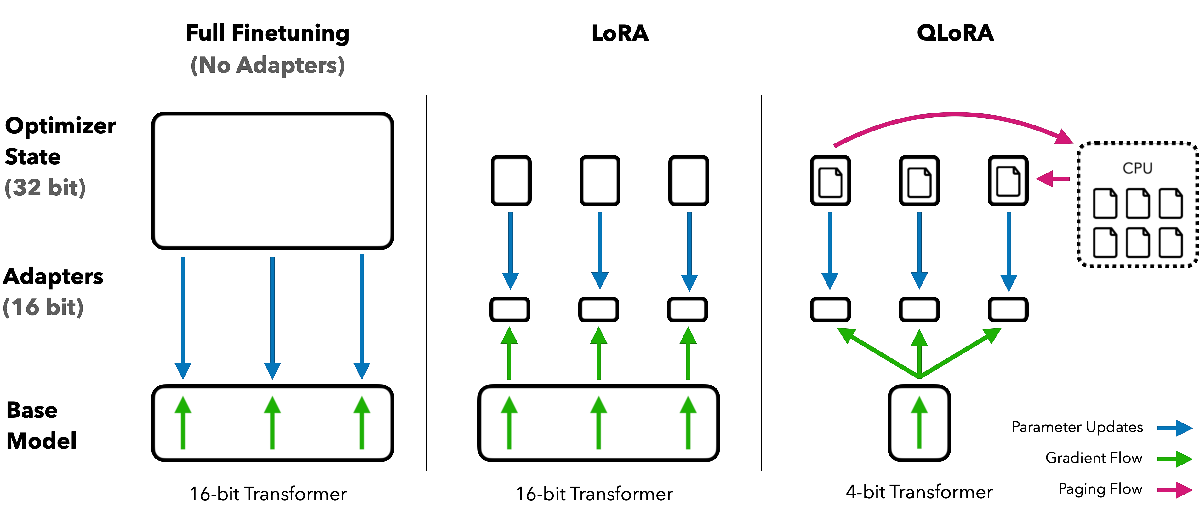
\includegraphics[width=\linewidth]{images/03_qlora}
    \caption[Comparison of the fine-tuning methods]{Comparison of the fine-tuning methods \parencite{Dettmers2023}}
    \label{fig:03_qlora}
\end{figure}


\section{Other Technologies}

\subsection{PyTorch}

\textbf{PyTorch}\footnote{https://pytorch.org/} is an open-source Python machine learning framework, originally developed by Meta, that is mainly designed for deep learning, including computer vision and natural language processing.
PyTorch implements many commonly used components of neural networks, such as linear layers, transformer layers, loss functions and optimizers.
These components enable fast design, training and deployment of models in a unified environment.

Broad GPU support is another great feature of PyTorch that allows most code to utilize GPU acceleration for faster model training and inference with minimal changes to the existing code, making its use fairly straightforward.
Multiple different GPU frameworks are supported, like NVIDIA CUDA, AMD ROCm and Intel XPU, with NVIDIA CUDA being the most widely used and optimized.

\subsection{HuggingFace}

\textbf{HuggingFace}\footnote{https://huggingface.co} is an open-source platform and community focused on machine learning.
It provides multiple tools and libraries for easier training, fine-tuning and distribution of models.

\subsubsection{HuggingFace Hub}

\textbf{HuggingFace Hub}\footnote{https://huggingface.co/docs/hub/index} is an online platform that allows the hosting of git repositories, models, datasets and hosting of demo apps (spaces), additionally to hosting, it also supports discussion and collaboration of users.
Currently, around 2 million models 500 thousand datasets are publicly available on the Hub, with many more being stored in private repositories.

Other HuggingFace libraries can then interface with the Hub, allowing the user to seamlessly access the hosted models and datasets through the code without the need for manual downloading.

\subsubsection{Transformers}

\textbf{Transformers}\footnote{https://huggingface.co/docs/transformers/en/index} is a library that contains many useful tools for interfacing with different machine learning models, providing a unified framework for both training and inference.
Transformers can be used to load models and datasets directly from the Hub and also contain useful abstractions, such as the Trainer class which implements a unified interface for passing parameters, monitoring and saving checkpoints during training.

\subsubsection{PEFT}

\textbf{PEFT}\footnote{https://huggingface.co/docs/peft/index} (Parameter-Efficient Fine-Tunig) is a library that implements efficient fine-tuning mechanisms for large pretrained models, such as \textbf{LoRA} and \textbf{QLoRA}.


\section{Experimental Environment}

Several experimental environments with GPU support were set up and tried for the modelling tasks.

\begin{itemize}
    \item \textbf{Betelgeuse server} (Astronomical Institute of the Czech Academy of Sciences) - equipped with 1x Nvidia GTX 980 GPU (4GB VRAM, released 2017), it delivers decent training performance, suitable for smaller experiments.
    \item \textbf{RCI Cluster} - while equipped with multiple Nvidia A100 GPUs (40GB VRAM, released 2020), we have found out that requesting access to even one GPU usually takes around an hour, with multiple GPUs being practically inaccessible due to the lower priority of the account, making the environment unsuitable for prototyping and exploring various model architectures.
    Nonetheless, we used the account at RCI cluster for sharing the large light curve datasets and the access to a large distributed computing platform provided us with valuable experience.
    \item \textbf{Author's PC} - equipped with 1x AMD Radeon RX9070 (16GB VRAM, released 2025) provides superior computational performance to the Betelgeuse server and better accessibility than the RCI cluster, it was therefore chosen as the primary experimental environment for our modeling tasks.
\end{itemize}




    \chapter{Experiment -- Classification of ECG Signals}

Before delving into the classification of astronomical light curves, we decided to run a similar experiment on a well-known dataset where transformer-based classifiers previously demonstrated remarkable results.  \parencite{Hu2022,ECGformer}


\section{Introduction}\label{sec:04_cntroduction}

We decided to use the MIT-BIH dataset \parencite{MIT-BIH} which is freely available via PhysioNet \parencite{PhysioNet} because we determined that the classification of ECG signals has some key similarities with the classification of astronomical light curves.
Mainly long-term relationships in the data and asymmetrical class distribution are especially relevant for our use-case.

The main purpose of this experiment was to get familiarity and hands-on experience with transformer-based models, architectures and relevant libraries (PyTorch, transformers) on an already explored and documented problem and later apply the acquired knowledge to the classification of astronomical light curves.


\section{Dataset}\label{sec:04_dataset}

The dataset consists of 48 half-hour two-channel ambulatory ECG recordings obtained from 47 patients studied by the BIH Arrhythmia Laboratory between 1975 and 1979.
The recordings were sampled at a frequency of 360Hz with at least two cardiologists annotating each record independently.
Each beat was annotated this way according to the AAMI EC57 standard, \footnote{\url{https://archive.physionet.org/physiobank/database/html/mitdbdir/intro.htm}} resulting in approximately 109,000 human-labeled datapoints. \parencite{MIT-BIH}

Like many other authors \parencite{Hu2022,ECG-CNN,ECGformer} we also mapped the labeled data to 5 classes.

\begin{table}[H]
    \centering
    \small
    \renewcommand{\arraystretch}{1.1}

    \begin{tabularx}{\textwidth}{X c@{\hspace{3em}}c}
        \toprule
        \textbf{Class (\textbf{Label})} & \textbf{Count} & \textbf{\%} \tabularnewline
        \midrule
        Normal (\textbf{N})                & 90594 & 82.77 \tabularnewline
        Supraventricular (\textbf{S})      & 2781  & 2.54  \tabularnewline
        Premature Ventricular (\textbf{V}) & 7235  & 6.61  \tabularnewline
        Fusion (\textbf{F})                & 802   & 0.73  \tabularnewline
        Unknown (\textbf{Q})               & 8030  & 7.35  \tabularnewline
        \bottomrule
    \end{tabularx}

    \caption[MIT-BIH Class distribution]{Class distribution.}
    \label{tab:04_classes}
\end{table}

\FloatBarrier

\subsection{Class Imbalance}\label{subsec:04_class-imbalance}

The class distribution shows a heavily imbalanced dataset, with the majority class (\textbf{N}) accounting for most samples and the other classes having only limited representation.
Such imbalance is typical of medical datasets, where pathological cases are usually rare and most of the screened population shows healthy behavior.

The objective of the machine learning models is then to identify these abnormalities to find individuals that need further screening or treatment.
In this context, maximizing recall is often preferred over accuracy as errors involving minority classes may have severe, potentially fatal consequences, while errors involving the majority (healthy) class carry little risk. \parencite{Hicks2022}

\begin{figure}[!htbp]
    \centering
    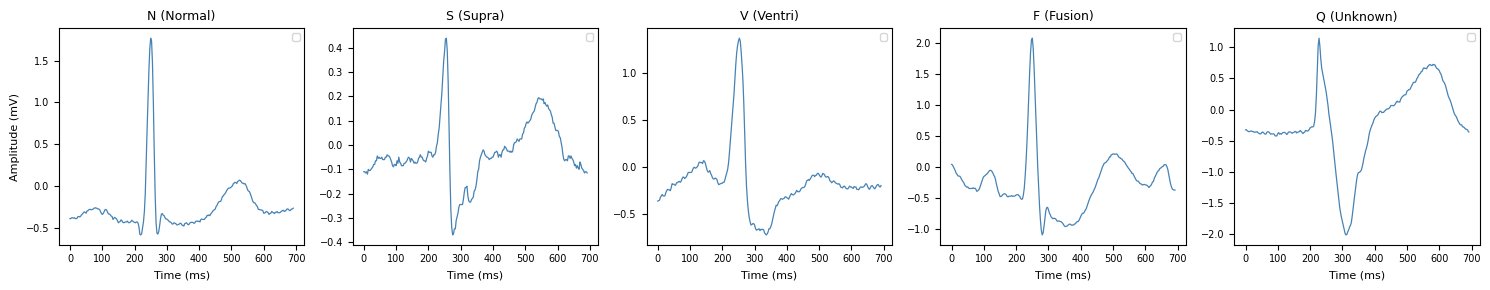
\includegraphics[width=\linewidth]{images/04_examples}
    \caption[MIT-BIH Examples]{MIT-BIH examples for each class.}
    \label{fig:04_examples}
\end{figure}

\subsection{Preprocessing}

Since the MIT-BIH dataset is sufficiently cleaned, little preprocessing was needed.
We have split each of the recordings into individual beats of length $250$, each beat was centered around its annotated peak.
Then a per-beat (per-sample) z-score transformation was applied to ensure each beat has a mean of 0 and a standard deviation of 1.

\begin{align}
    Z = \frac{X - \overline{X}}{\mu}
\end{align}

\begin{center}
    \small Z-score transformation of a variable $X$
\end{center}


\section{Methodology}\label{sec:04_methodology}

In order for the experiments to produce models that are generalizable - perform well on new, unseen data, we must first describe the methodology used for training, evaluation and selection of these models.
The experiments should also be replicable, therefore we use RNG seeding and document all the relevant parameters and configurations for each model.

\subsection{Metric definition}

Since the experiments will be focused on multi-class classification, It is necessary to define the relevant metrics.

\bigskip

\noindent First we define per-class TP, FP, TN, FN as:

\begin{table}[H]
    \centering
    \scriptsize
    \renewcommand{\arraystretch}{1.1}

    \begin{tabularx}{\textwidth}{X c}
        \toprule
        \textbf{Metric} & \textbf{Definition} \tabularnewline \midrule
        $\mathrm{TP}_c$ & \# of instances of class $c$ that were classified as class $c$ \tabularnewline
        $\mathrm{FP}_c$ & \# of instances of classes other than $c$ that were classified as class $c$ \tabularnewline
        $\mathrm{TN}_c$ & \# of instances of classes other than $c$ that were classified as class other than $c$ \tabularnewline
        $\mathrm{FN}_c$ & \# of instances of class $c$ that were classified as class other than $c$ \tabularnewline
        \bottomrule
    \end{tabularx}

    \caption[TP, FP, TN, FN definition]{TP, FP, TN, FN definition.}
    \label{tab:04_tp_fp_tn_fn}
\end{table}

\FloatBarrier

Then we define per-class Precision, Recall and F1-score as:

        {\setlength{\jot}{1em}
\begin{align}
    \mathrm{Precision}_c &= \frac{\mathrm{TP}_c}{\mathrm{TP}_c + \mathrm{FP}_c} \\
    \mathrm{Recall}_c &= \frac{\mathrm{TP}_c}{\mathrm{TP}_c + \mathrm{FN}_c} \\
    \mathrm{F1}_c &= 2 \cdot \frac{\mathrm{Precision}_c \cdot \mathrm{Recall}_c}{\mathrm{Precision}_c + \mathrm{Recall}_c}
\end{align}
}

\begin{center}
    \small Per-class metrics
\end{center}

\bigskip

\noindent We then further define Macro and Weighted Precision, Recall and Macro F1-score (Macro F1) as arithmetic and weighted means of per-class metrics respectively:

        {\setlength{\jot}{1em}
\begin{align}
    \mathrm{Macro Precision} &= \frac{1}{C} \sum^{C}{\mathrm{Precision}_c} \\
    \mathrm{Macro Recall} &= \frac{1}{C} \sum^{C}{\mathrm{Recall}_c} \\
    \mathrm{Macro \, F1} &=  \frac{1}{C} \sum^{C}{\mathrm{F1}_c}
\end{align}

\begin{center}
    \small Macro metrics
\end{center}

\begin{align}
    \mathrm{Weighted Precision} &=  \frac{\sum^{C}{w_c \cdot \mathrm{Precision}_c}}{\sum^{C}{w_c}} \\
    \mathrm{Weighted Recall} &=  \frac{\sum^{C}{w_c \cdot \mathrm{Recall}_c}}{\sum^{C}{w_c}} \\
    \mathrm{Weighted F1} &= \frac{\sum^{C}{w_c \cdot \mathrm{F1}_c}}{\sum^{C}{w_c}}
\end{align}
}

\begin{center}
    \small Weighted metrics
\end{center}

Where $C$ is the number of classes and $w_c$ the number of instances of the class~$c$.

\subsection{Model evaluation}

We adopt the standard \textbf{train}/\textbf{validation}/\textbf{test} protocol for model development and evaluation.
Specifically, the dataset is partitioned into three subsets: \textbf{train}, \textbf{val} and \textbf{test}.

We don't take the individual recordings into account, this allows different beats from one recording to end up in different subsets.
While this approach wouldn't be ideal for real world applications, many other authors use it in their works\parencite{Hu2022, ECGformer}, and it allows us to compare our results to theirs.

\textbf{Model training} is then performed exclusively on the \textbf{train} subset while performance is evaluated\footnote{Evaluation refers to the computation of metrics.} on the \textbf{val} subset after each \textbf{epoch}\footnote{One complete pass over the \textbf{train} subset during training.}.
Based on these validation results, we select the best model \textbf{checkpoint}\footnote{The state of the model after \(n\) epochs.}, primarily according to a chosen performance metric and the discrepancy between \textbf{train} and \textbf{val} performance (large gap typically indicates overfitting).

The selected final checkpoint is then evaluated on the \textbf{test} subset, which serves as an approximation of performance on previously unseen data.
Throughout preprocessing, special care must be taken to prevent information leakage into the \textbf{test} subset.

As a main performance metric for selection of our classifier models we've decided to choose Macro F1.
While we've previously discussed the importance of Recall in medical applications Macro F1 is used as a main metric in many other publications \parencite{Hu2022} and will allow us to effectively compare our models against other solutions.
At the same time, Macro F1 still places strong emphasis on Recall through its harmonic formulation, making it aligned with our objective of accurately identifying important minority classes.


\section{Experiments}

We've performed multiple experiments with various transformer-based classifiers and different configurations / parameters for each model.
For clarity, we show only the configurations that performed well or were otherwise interesting.

\subsection{Weighted Loss}\label{subsec:04-weighted-loss}

Due to the imbalance of classes in the dataset a commonly used \textbf{Cross-Entropy Loss} ($L_{\mathrm{CE}}$) performed badly on the data.
Because of this, we've decided to adopt \textbf{Weighted Cross-Entropy Loss} ($L_{\mathrm{WCE}}$) which mitigates the imbalance by taking the class weights into account.

\begin{align}
    L_{\mathrm{CE}}(Y, \hat{p}) &= - \sum_{c=1}^{C} y_c \log \hat{p}_c \label{eq:04-cross-entropy} \\
    L_{\mathrm{WCE}}(Y, \hat{p}) &= - \sum_{c=1}^{C} \alpha_c \, y_c \log \hat{p}_c \label{eq:04-weighted-cross-entropy}
\end{align}

\subsection{Base Transformer}\label{subsec:04-base-transformer}

As the first configuration, we trained an encoder-only transformer model from scratch.

\subsubsection{Architecture}

\begin{enumerate}
    \item The ECG signal of length \textbf{250} was tokenized into \textbf{25} non-overlapping patches of size \textbf{10}.
    \item These tokens are then projected into dimension $d_{\mathrm{model}}$ using a linear layer, positional embeddings are also added.
    \item A learnable classification (CLS) token is then appended and the entire sequence is put through the encoder blocks.
    \item Then, the last token is extracted (last token pooling) and using a linear classifier layer, probability logits are obtained.
\end{enumerate}

The following model configuration was used:

\FloatBarrier

\begin{table}[H]
    \centering
    \small
    \renewcommand{\arraystretch}{1.1}

    \begin{tabularx}{0.6\textwidth}{X c}
        \toprule
        \textbf{Parameter} & \textbf{Value} \tabularnewline
        \midrule
        $d_{\mathrm{model}}$ & $256$ \tabularnewline
        $d_{\mathrm{ff}}$    & $1024$ \tabularnewline
        $n_{\mathrm{head}}$  & $8$ \tabularnewline
        $n_{\mathrm{layer}}$ & $8$ \tabularnewline
        Activation Function & ReLU \tabularnewline
        \bottomrule
    \end{tabularx}

    \caption[Base Transformer Configuration]{Base Transformer Configuration.}
    \label{tab:04_base_transformer_configuration}
\end{table}

\FloatBarrier

\subsubsection{Training}

The training took around 5 minutes, the following parameters were used:

\begin{table}[H]
    \centering
    \small
    \renewcommand{\arraystretch}{1.1}

    \begin{tabularx}{0.6\textwidth}{X c}
        \toprule
        \textbf{Parameter} & \textbf{Value} \tabularnewline
        \midrule
        Epochs        & $100$ \tabularnewline
        Learning Rate & $5 \times 10^{-5}$ \tabularnewline
        Batch Size    & $128$ \tabularnewline
        Dropout       & $0.15$ \tabularnewline
        Loss          & WeightedLoss \tabularnewline
        Optimizer     & AdamW \tabularnewline
        Weight Decay  & $1 \times 10^{-2}$ \tabularnewline
        \bottomrule
    \end{tabularx}

    \caption[Base Transformer Training Parameters]{Training Parameters.}
    \label{tab:04_base_transformer_training}
\end{table}

\FloatBarrier

Previous work by \textcite{Hu2022, ECGformer} was used as the basis for the used hyperparameters.

Training loss continued to decrease over the training, the training and validation loss diverged at around epoch $20$ and validation loss started increasing at around epoch $40$.
Validation Macro F1 reached the best value at epoch $53$ and stagnated afterward.

\begin{figure}[!htbp]
    \centering
    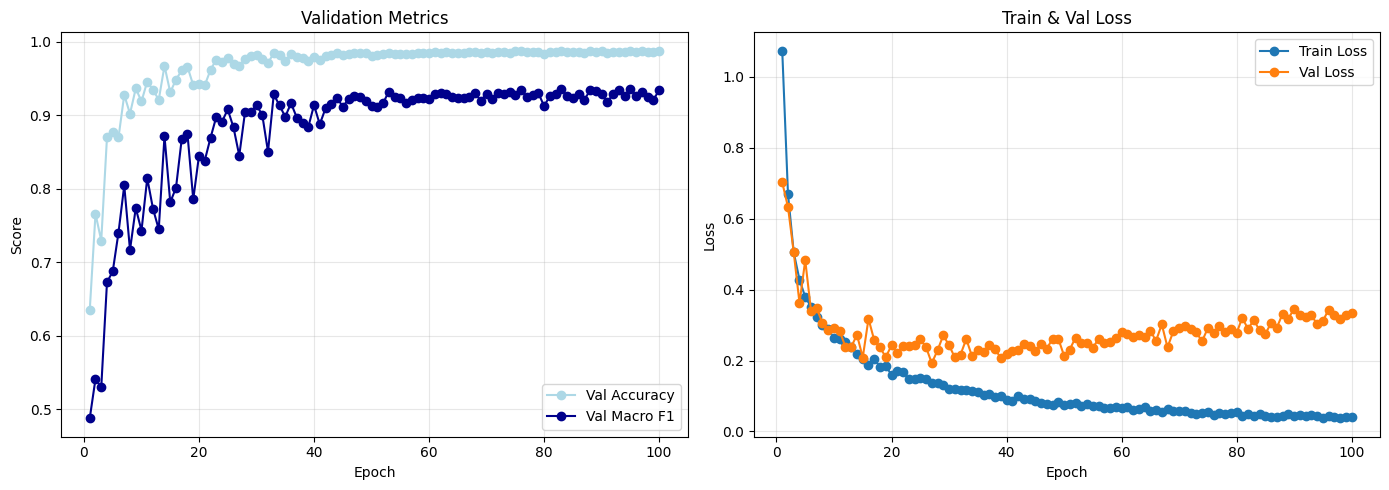
\includegraphics[width=0.9\linewidth]{images/04/base_transformer_training_curves}
    \caption[Base Transformer Training Curves]{Training Curves.}
    \label{fig:04_base_transformer_training_curves}
\end{figure}

\FloatBarrier

\subsubsection{Evaluation}


Checkpoint at epoch $53$ was chosen for detailed evaluation on the \textbf{val} set due to its best Macro F1.

\begin{table}[H]
    \centering
    \footnotesize
    \renewcommand{\arraystretch}{1.1}

    \begin{minipage}[t]{0.32\textwidth}
        \centering
        \begin{tabularx}{\textwidth}{X c}
            \toprule
            \textbf{Metric} & \textbf{Score} \tabularnewline
            \midrule
            Accuracy    & 0.9853 \tabularnewline
            Macro F1    & 0.9320 \tabularnewline
            Weighted F1 & 0.9856 \tabularnewline
            \bottomrule
        \end{tabularx}
    \end{minipage}
    \hfill
    \begin{minipage}[t]{0.64\textwidth}
        \centering
        \footnotesize
        \begin{tabularx}{\textwidth}{X c c c c}
            \toprule
            \textbf{Class} & \textbf{Precision} & \textbf{Recall} & \textbf{F1-score} & \textbf{Support} \tabularnewline
            \midrule
            N & 1.00 & 0.99 & 0.99 & 19025 \tabularnewline
            S & 0.80 & 0.91 & 0.85 & 584   \tabularnewline
            V & 0.95 & 0.98 & 0.97 & 1519  \tabularnewline
            F & 0.85 & 0.88 & 0.86 & 169   \tabularnewline
            Q & 0.99 & 1.00 & 0.99 & 1688  \tabularnewline
            \bottomrule
        \end{tabularx}
    \end{minipage}

    \caption[Base Transformer Evaluation Metrics]{Evaluation Metrics.}
    \label{tab:04_base_transformer_evaluation_metrics}
\end{table}

\FloatBarrier

\begin{figure}[!htbp]
    \centering
    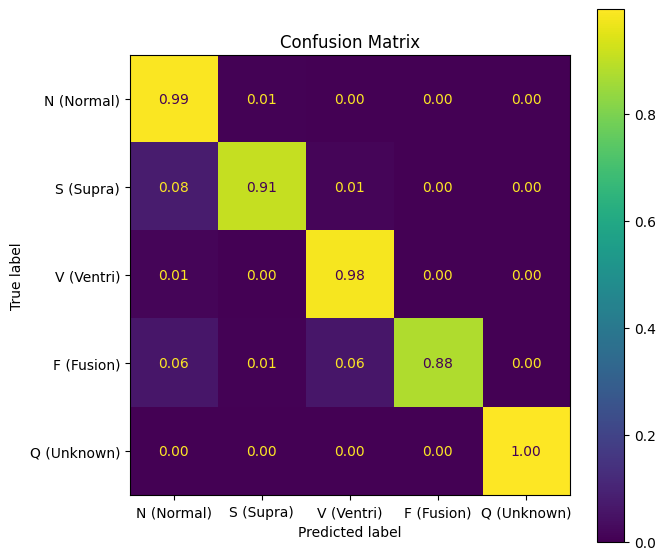
\includegraphics[width=0.6\linewidth]{images/04/base_transformer_confusion_matrix}
    \caption[Base Transformer Confusion Matrix]{Confusion Matrix.}
    \label{fig:04_base_transformer_confusion_matrix}
\end{figure}

\FloatBarrier

The baseline model performed excellently at $\mathrm{Macro \, F1} = 0.93$.
Additionally, we can see that the model achieved per-class performance at rate proportional to the class's support with classes \textbf{S} and \textbf{F} having the worst scores.

\subsection{Qwen2.5 0.5B fine-tune}

For the next experiment we've performed a LoRA fine-tune of pretrained a Qwen2.5 0.5B\footnote{https://huggingface.co/Qwen/Qwen2.5-0.5B} \parencite{qwen2025} LLM\@.
The size of 0.5B (500 million parameters) made it small enough to effectively fine-tune on available hardware (AMD Radeon RX 9070 GPU).

\subsubsection{Architecture}

We used the same approach for tokenization and embedding as in the first experiment, entirely bypassing the original tokenizer and embedding layer.
A learnable CLS token with the classification layer was also implemented, resulting in nearly identical architecture to the first experiment, only difference being the pretrained transformer stack.

\begin{table}[H]
    \centering
    \small
    \renewcommand{\arraystretch}{1.1}

    \begin{tabularx}{0.6\textwidth}{X c}
        \toprule
        \textbf{Parameter} & \textbf{Value} \tabularnewline
        \midrule
        $d_{\mathrm{model}}$ & $896$ \tabularnewline
        $d_{\mathrm{ff}}$    & $4864$ \tabularnewline
        $n_{\mathrm{head}}$  & $16$ \tabularnewline
        $n_{\mathrm{layer}}$ & $24$ \tabularnewline
        Activation Function & SwiGLU \tabularnewline
        \bottomrule
    \end{tabularx}

    \caption[Qwen 2.5 0.5B Configuration]{Configuration.}
    \label{tab:04_qwen2.5_0.5b_configuration}
\end{table}

\FloatBarrier

\subsubsection{Training}

The training took around 90 minutes, the following parameters were used:

\begin{table}[H]
    \centering
    \small
    \renewcommand{\arraystretch}{1.1}

    \begin{tabularx}{0.6\textwidth}{X c}
        \toprule
        \textbf{Parameter} & \textbf{Value} \tabularnewline
        \midrule
        Epochs        & $30$ \tabularnewline
        Learning Rate & $5 \times 10^{-5}$ \tabularnewline
        Batch Size    & $128$ \tabularnewline
        Dropout       & $0.15$ \tabularnewline
        Loss          & WeightedLoss \tabularnewline
        Optimizer     & AdamW \tabularnewline
        Weight Decay  & $1 \times 10^{-2}$ \tabularnewline
        LoRA rank     & $8$ \tabularnewline
        LoRA $\alpha$ & $16$ \tabularnewline
        \bottomrule
    \end{tabularx}

    \caption[Qwen 2.5 0.5B Training Parameters]{Training Parameters.}
    \label{tab:04_qwen_2.5_0.5b_training}
\end{table}

\FloatBarrier

The model started converging much faster than in the first experiment, achieving $0.90$ validation Macro F1 in $7$, however after that point at around epoch $10$, the validation loss diverged from the training loss and immediately started increasing

\begin{figure}[!htbp]
    \centering
    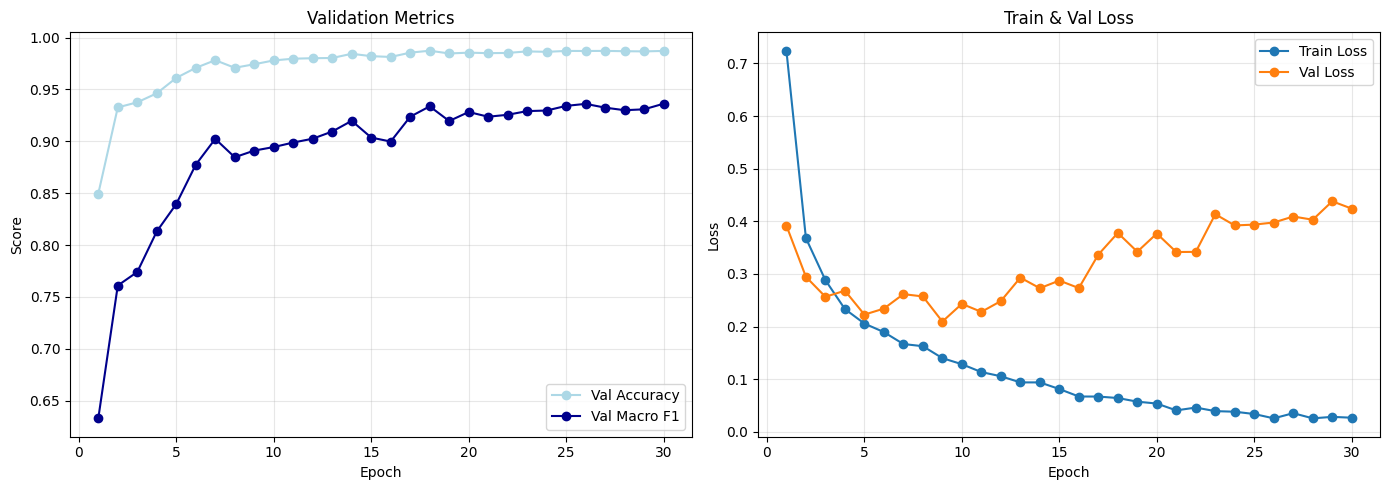
\includegraphics[width=0.9\linewidth]{images/04/llm_training_curves}
    \caption[Qwen 2.5 0.5B Training Metrics]{Training Metrics.}
    \label{fig:04_qwen_2.5_0.5b_training_metric}
\end{figure}

\FloatBarrier

\subsubsection{Evaluation}

Checkpoint at epoch $7$ was chosen for further evaluation on val dataset as the best model due to its best val Macro F1 before divergence and probable overfitting started happening.

\begin{table}[H]
    \centering
    \footnotesize
    \renewcommand{\arraystretch}{1.1}

    \begin{minipage}[t]{0.32\textwidth}
        \centering
        \begin{tabularx}{\textwidth}{X c}
            \toprule
            \textbf{Metric} & \textbf{Score} \tabularnewline
            \midrule
            Accuracy    & 0.9782 \tabularnewline
            Macro F1    & 0.9024 \tabularnewline
            Weighted F1 & 0.9787 \tabularnewline
            \bottomrule
        \end{tabularx}
    \end{minipage}
    \hfill
    \begin{minipage}[t]{0.64\textwidth}
        \centering
        \footnotesize
        \begin{tabularx}{\textwidth}{X c c c c}
            \toprule
            \textbf{Class} & \textbf{Precision} & \textbf{Recall} & \textbf{F1-score} & \textbf{Support} \tabularnewline
            \midrule
            N & 0.99 & 0.98 & 0.99 & 19025 \tabularnewline
            S & 0.73 & 0.86 & 0.79 & 584   \tabularnewline
            V & 0.92 & 0.98 & 0.94 & 1519  \tabularnewline
            F & 0.80 & 0.80 & 0.80 & 169   \tabularnewline
            Q & 0.99 & 0.99 & 0.99 & 1688  \tabularnewline
            \bottomrule
        \end{tabularx}
    \end{minipage}

    \caption[Qwen 2.5 0.5B Evaluation Metrics]{Evaluation Metrics.}
    \label{tab:04_qwen_2.5_0.5b_evaluation_metrics}
\end{table}

\FloatBarrier

\begin{figure}[!htbp]
    \centering
    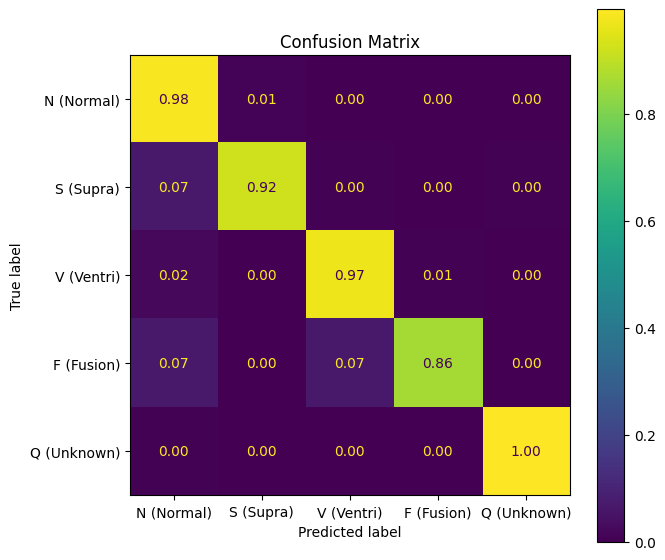
\includegraphics[width=0.6\linewidth]{images/04_qwen_2.5_0.5b_confusion_matrix}
    \caption[Qwen 2.5 0.5B Confusion Matrix]{Confusion Matrix.}
    \label{fig:04_qwen_2.5_0.5b_confusion_matrix}
\end{figure}

\FloatBarrier


\section{Results and Discussion}

The first base transformer outperformed the second LLM fine-tune model and its checkpoint at epoch $53$ was therefore chosen as the model for final evaluation on the \textbf{test} set.

\begin{table}[H]
    \centering
    \footnotesize
    \renewcommand{\arraystretch}{1.1}

    \begin{minipage}[t]{0.32\textwidth}
        \centering
        \begin{tabularx}{\textwidth}{X c}
            \toprule
            \textbf{Metric} & \textbf{Score} \tabularnewline
            \midrule
            Accuracy    & 0.9839 \tabularnewline
            Macro F1    & 0.9253 \tabularnewline
            Weighted F1 & 0.9843 \tabularnewline
            \bottomrule
        \end{tabularx}
    \end{minipage}
    \hfill
    \begin{minipage}[t]{0.64\textwidth}
        \centering
        \footnotesize
        \begin{tabularx}{\textwidth}{X c c c c}
            \toprule
            \textbf{Class} & \textbf{Precision} & \textbf{Recall} & \textbf{F1-score} & \textbf{Support} \tabularnewline
            \midrule
            N & 1.00 & 0.99 & 0.99 & 8154 \tabularnewline
            S & 0.77 & 0.93 & 0.84 & 250  \tabularnewline
            V & 0.94 & 0.97 & 0.96 & 651  \tabularnewline
            F & 0.84 & 0.85 & 0.84 & 72   \tabularnewline
            Q & 0.99 & 0.99 & 0.99 & 724  \tabularnewline
            \bottomrule
        \end{tabularx}
    \end{minipage}

    \caption[Final Model Evaluation Metrics]{Final Model Evaluation Metrics.}
    \label{tab:04_final_model_evaluation_metrics}
\end{table}

\FloatBarrier

\begin{figure}[!htbp]
    \centering
    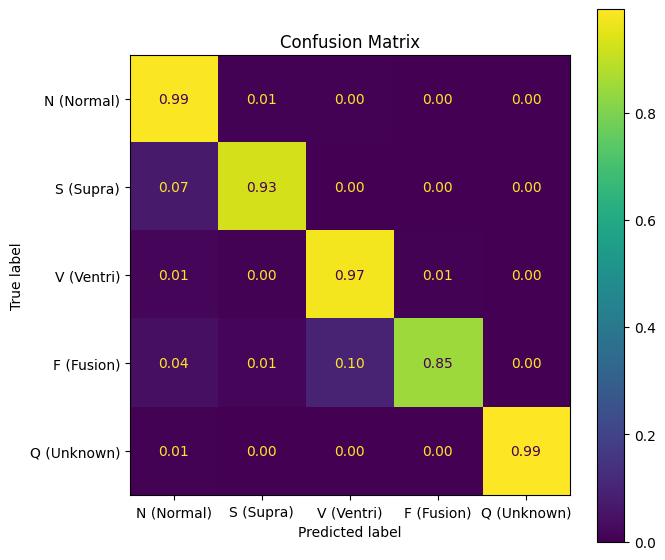
\includegraphics[width=0.6\linewidth]{images/04/test_confusion_matrix}
    \caption[Final Model Confusion Matrix]{Final Model Confusion Matrix.}
    \label{fig:final_model_confusion_matrix}
\end{figure}

\FloatBarrier

The final model performed only slightly worse on the unseen test data ($\Delta \mathrm{Macro \, F1} \leq 0.01$) and has shown that transformer-based models are suitable for the classification of time series.

The LLM fine-tune solution still performed surprisingly well and shows that even older and very small LLMs can achieve performance comparable to specialized models.
With more modern and larger models (like Qwen3.6 series) the performance might've been even better, however such experiments are costly due to the immense computational costs of fine-tuning (larger models require clusters of high-end GPUs even for a (Q)LoRA fine-tune).

\subsection{Comparison with Other Work}

Additionally, we provide a comparison of our models with the work of other authors.

\begin{table}[ht]
    \centering
    \small
    \renewcommand{\arraystretch}{1.1}
    \begin{tabularx}{\textwidth}{Xcccc}
        \toprule
        \textbf{Model} & \textbf{Macro F1 Score} & \textbf{Accuracy} & \textbf{Method} \tabularnewline \midrule
        \cite{Hu2022} ($\alpha$) & 0.94 & 0.99 & Transformer \tabularnewline
        Base Transformer & 0.93 & 0.98 & Transformer \tabularnewline
        Qwen 2.5 0.5B fine-tune & 0.90 & 0.98 & LoRA fine-tune \tabularnewline
        \cite{Mousavi2021} & 0.87 & 0.98 & ELP + CNN \tabularnewline
        \cite{ECGformer} & 0.86 & 0.98 & Transformer \tabularnewline
        \bottomrule
    \end{tabularx}
    \caption[Comparison of Results]{Comparison of different models, ordered by Macro F1 Score.}
    \label{tab:04_comparison_of_results}
\end{table}










    \chapter{TESS Light Curve Dataset}

\section{TESS Mission}

TESS (Transiting Exoplanet Survey Satellite) \parencite{Ricker2014} is a satellite launched by NASA in 2018.
While its primary mission is the discovery of exoplanets, TESS monitors all objects that exhibit signs of changing brightness, including variable stars.

The satellite is equipped with four 16 megapixel wide-field cameras, producing high-quality full-frame images.
Individual objects are then identified and target pixel files (TPFs) are created.

Light curves are then obtained by calculating flux from the TPFs for each object and assembling them into time-series, each data product is then given a unique TIC - a numerical identifier.\parencite{TESSDataProducts}


\begin{figure}[!htbp]
    \centering
    \includegraphics[width=0.7\linewidth]{images/05/tess_satellite}
    \caption[TESS Satellite]{The TESS satellite before its launch in 2018. \parencite{tess_satellite}}
    \label{fig:05_tess_satellite}
\end{figure}

\FloatBarrier


\section{Dataset}

Mgr.\,Marek Skarka\,Ph.D. (Astronomical Institute of the Czech Academy of Sciences) generously provided us with a cleaned subset of a manually labeled dataset from the northern TESS viewing zone, for full details concerning the original dataset see \cite{Skarka2022}.

\subsection{Classes}

The original dataset contains \textbf{3402} total light curves with various annotations.
In total, \textbf{49} different classes are present with only \textbf{13} having more than \textbf{10} samples.

The classes were then combined into \textbf{5} main superclasses.
Samples with multiple annotations spanning multiple superclasses like ROTM\slash ELL (Rotating\slash Eclipsing) or extremely rare classes like HB (\hyperref[item:02-horiozntal-branch]{Horizontal Branch star}) were discarded, since they constituted only a small fraction of the entire dataset (\textbf{55} samples), leaving \textbf{3347} light curves.

\begin{table}[H]
    \centering
    \footnotesize
    \renewcommand{\arraystretch}{1.1}
    \begin{tabularx}{\textwidth}{X c@{\hspace{3em}}c@{\hspace{3em}}c}
            \toprule
            \textbf{Class (Label)} & \textbf{Original Labels} & \textbf{Count} & \textbf{Total} \tabularnewline \midrule
            Non-Variable (\textbf{N}) & NONE & \num{1729} & \num{1729}   \tabularnewline \midrule
            Unspecified-Variable (\textbf{U})             & VAR & 720 & 720    \tabularnewline \midrule
            Pulsating (\textbf{P}) &
            \begin{tabular}{@{}c@{}}
                GDOR \\ DSCT+GDOR \\ GDOR+DSCT \\ DSCT
            \end{tabular} &
            \begin{tabular}{@{}c@{}}
                206 \\ 176 \\ 86 \\ 67
            \end{tabular} &
            535    \tabularnewline \midrule
            Rotating (\textbf{R}) &
            \begin{tabular}{@{}c@{}}
                ROTS \\ ROT \\ ROTM
            \end{tabular} &
            \begin{tabular}{@{}c@{}}
                175 \\ 74 \\ 13
            \end{tabular} &
            262    \tabularnewline \midrule
            Eclipsing (\textbf{E}) &
            \begin{tabular}{@{}c@{}}
                EA \\ ELL \\ EW \\ EB
            \end{tabular} &
            \begin{tabular}{@{}c@{}}
                47 \\ 24 \\ 17 \\ 13
            \end{tabular} &
            101    \tabularnewline \midrule
            Total & & & \num{3347} \tabularnewline
            \bottomrule
    \end{tabularx}
    \caption[TESS Dataset Classes]{The TESS light curve dataset with simplified labels.}
    \label{tab:05_base_class_counts}
\end{table}

\FloatBarrier

We provide a brief description of the original labels, full explanation is provided in the original article by~\cite{Skarka2022}.

\begin{itemize}
    \item \textbf{NONE} - Star shows no signs of variability.
    \item \textbf{VAR} - Star shows signs of variability, but the exact class couldn't be identified accurately.
    \item \textbf{CLASS} - Variability type as described in ~\hyperref[sec:02-variable-stars]{2.4 Variable Stars}, for example a \textbf{DSCT} annotation would refer to a ~\hyperref[subsubsec:02-dsct]{Delta Scuti} star.
    \item \textbf{CLASS1+CLASS2} - Combined class, shows mainly signs of the first class.
    \item \textbf{CLASS1/CLASS2} - Uncertain class, the star could be of either of the classes.
\end{itemize}

\subsection{Light Curves}

The light curves were recorded at a 2-minute cadence and have various lengths, ranging roughly from $\num{11000}$ to $\num{216000}$ observations.

In their raw form, the curves contain only a timestamp ($t$), flux measurement ($\Phi$) and error measurement ($\Phi_{err}$).
By default, TESS data products measure time in Barycentric TESS Julian Days (BTJD), with $\mathrm{BTJD} = 0$ corresponding to roughly midnight on 01/01/2015.

\begin{figure}[!htbp]
    \centering
    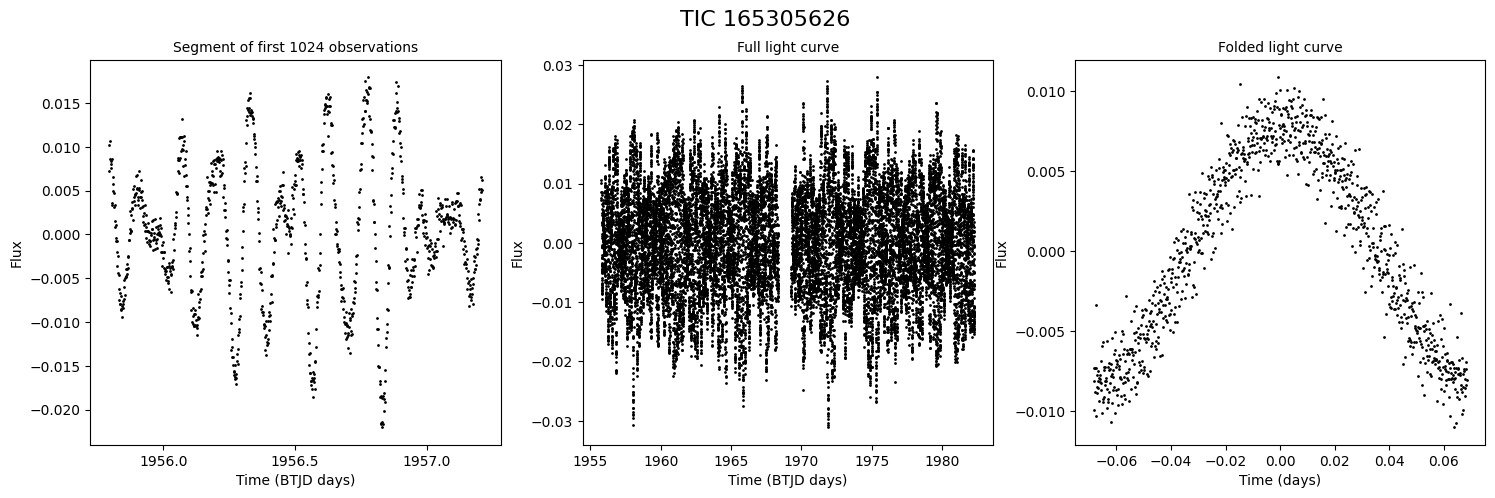
\includegraphics[width=\linewidth]{images/05_raw_light_curve}
    \caption[RAW Light Curve]{Raw light curve of a DSCT star, note the observation gap in the middle of the full light curve.}
    \label{fig:05_raw_light_curve}
\end{figure}

\FloatBarrier


\section{Preprocessing}

The original light curves were provided as a files in .csv format, each file representing a different light curve.

Raw light curves are not suitable for direct model ingestion due to their length, observation gaps and instrumental trends, additional preprocessing steps must therefore be taken to prepare the data.

Many different preprocessing approaches were tried and tested with different models producing various results, some of the preprocessing steps didn't yield any performance improvements and were therefore not used in the showcased models in the next chapter.
We therefore describe our approach of selecting appropriate preprocessing steps and extracting valuable information in the data while also discussing which preprocessing steps were unsuitable for the task.

\subsection{Time Standardization}

Since different light curves might have different starting times $t_0$, we need to remap the time axis to a common reference point, making the light curves comparable.
Zero was chosen as the time of the first observation, so all curves start at $t=0$.

\[
    t' = t - t_0
\]

\subsection{Flux Normalization}

Experiments have shown that the transformers perform better when the flux values are normalized, so we applied a modified \textbf{min-max normalization} to the \textbf{flux} ($\Phi$) values of each light curve.
The modified min-max normalization maps the flux values into range of $[-1, 1]$ instead of the more traditional range of $[0, 1]$, we have chosen this approach because it better represent the physical nature of the data where the flux oscillates above and below the zero centered norm.

\[
    \Phi' = 2 \cdot \frac{\Phi - \Phi_{\min}}{\Phi_{\max} - \Phi_{\min}} - 1
\]

We would like to add that experiments were performed with both mentioned types of normalization, however there were no measurable differences in predictive performance of the resulting models.

The normalization itself makes the various light curves comparable and allows for better generalization of the model, since the variability type is mainly distinguishable by the morphology of the light curve and not its amplitude.
The amplitude is extracted before normalization and stored as scalar value that can be utilized by combined models that are not strictly transformer based.

\subsection{Detrending}

Some form of detrending is often applied when preprocessing the light curves to remove instrumental noise, baseline drift and other low-frequency artifacts, however certain types of stars, particularly rotating variables, exhibit long-term patterns that are suppressed by the detrending algorithms.

Although multiple detrending algorithms were tried with various parameters, none of them yielded better results than the non-detrended original.

Flux detrending can be generally written as:

\[
    \Phi' = \Phi - \Phi_{\mathrm{trend}}
\]

Computation of $\Phi_{\mathrm{trend}}$ then depends on the detrending algorithm.

\subsubsection{Used Detrending Algorithms}

\begin{enumerate}
    \item \textbf{Running Median}
    \[
        \Phi_{\mathrm{trend}}(t_i) = \mathrm{median}\{\Phi(t_j): t_j \in [t_i - w/2, t_i + w/2]\}
    \]
    Where $w$ is the size of the sliding window where median is computed.
    \item \textbf{Gaussian Smoothing}
    \[
        \Phi_{\mathrm{trend}} = G(\Phi;\sigma)
    \]
    Where $G(\Phi;\sigma)$ represents a convolution of the flux $\Phi$ with a 1D gaussian kernel with standard deviation $\sigma$.
    \item \textbf{Polynomial Detrending}
    \[
        \Phi_{\mathrm{trend}} = p(\Phi)
    \]
    Where $p(\Phi)$ is a polynomial approximation of $\Phi$, usually low-order.
\end{enumerate}

While detrending still remains a valuable tool for many tasks (i.e.~searching for eclipsing binaries), its performance for our task proved insufficient and was therefore removed from the final pipeline.

\subsection{Observation Gaps}\label{subsec:05-observation-gaps}

Masking was used to handle observation gaps that are present in the data.
During preprocessing, all points with invalid flux values (NaN, +inf, -inf) are identified and a binary mask is constructed (True signals a valid position).

The mask is then applied during attention, preventing the invalid positions from influencing other tokens.
If a CLS token is used for classification, no other modifications are needed (since it was not influenced by the invalid positions), however when mean token pooling is used, the mask must be applied a second time to prevent the invalid tokens from being pooled alongside the valid ones.

\begin{figure}[!htbp]
    \centering
    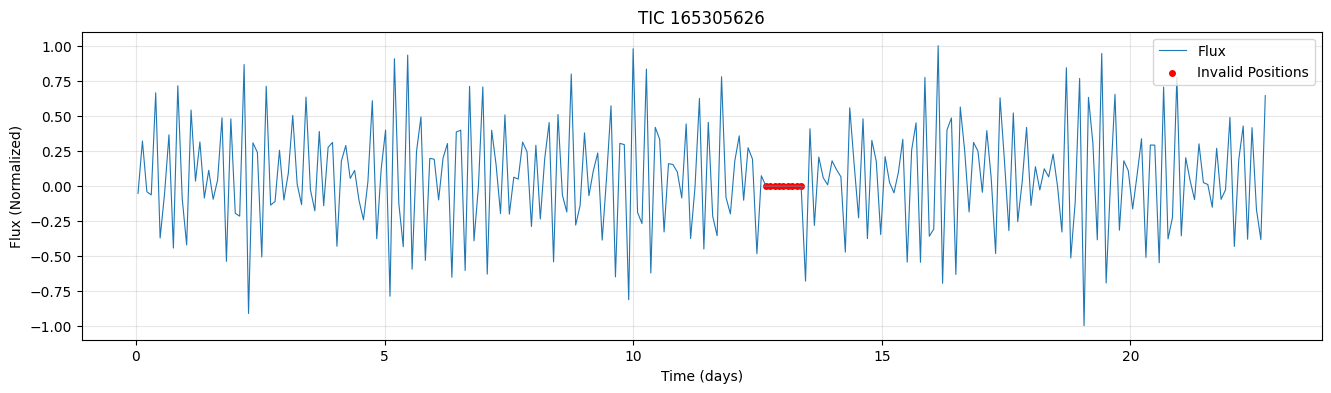
\includegraphics[width=\linewidth]{images/05/light_curve_invalid_positions}
    \caption[Observation Gap Masking]{A light curve with an identified observation gap (highlighted by red).}
    \label{fig:05_gap_masking}
\end{figure}

\FloatBarrier

\subsubsection{Handling Masks in Patch Embeddings}

When utilizing patch embeddings, additional measures must be taken to correctly apply the mask.

\subsection{Segmentation}

Since transformers have quadratic computation complexity with respect to the input sequence length \parencite{AttentionIsAllYouNeed}, feeding the entire light curves into the transformer quickly becomes infeasible\footnote{Training of a single-channel transformer on a dataset of $1000$ datapoints with length \num{4000} would take around $1$ minute per epoch. If a length \num{16000} (shortest light curves in the dataset) was used, the duration of one epoch would be roughly 16 minutes.}.
To address this issue, we tried various approaches that compact the light curves into more manageable form while preserving both local and global morphology.

\subsection{Multiple Time-domain Views}

As a solution to this problem, we propose providing the transformer model with multiple views of the given light curve, each having a different \textbf{temporal resolution}\footnote{Temporal resolution describes the amount of time that passes between observations - the measured flux ($\Phi$) values in our case. The default (highest) temporal resolution is 2-minutes in our dataset.}.
Multiple temporal resolutions allow us to capture periodic trends that are happening at different timescales while keep the individual views relatively short (our experiments have shown that $256$ is a good compromise of small size and high information content).

After several experiments, we decided to use the following 4 temporal resolutions for the views:

\begin{itemize}
    \item \textbf{2-minute resolution} (default)
    \item \textbf{8-minute resolution} ($\mathrm{bin\_size}=4$)
    \item \textbf{64-minute resolution} ($\mathrm{bin\_size}=16$)
    \item \textbf{128-minute resolution} ($\mathrm{bin\_size}=64$)
\end{itemize}

The views were then obtained by selecting an appropriate window from the light curve and mean-binning it to a specified fixed length that was same for all of the views.
For example, the 128-minute resolution view of size $256$ would be obtained by selecting a window of size

\[
    \frac{128 \, \mathrm{(resolution)}}{2 \, \mathrm{(default \, resolution)}} \cdot 256 \, \mathrm{(view \, size)} = \num{16384}
\]

then, mean-binning\footnote{The points are split into $n$ equally spaced, fixed-size bins ($n$ = 256, bin\_size = 64 in this case). A new sequence of length $n$ is then constructed where values at each position is the mean of all points in the corresponding bin.} the points in the window to length $256$ (size of $1$ bin would be $64$).

Each of the views starts at the beginning of the light curve / segment, this makes the smaller views subsequences of the larger views.
For example, assuming view size of $256$, the 2-minute resolution view becomes the first 4 points of the largest, lowest resolution 128-min view.

\begin{figure}[!htbp]
    \centering
    
\includegraphics[width=\linewidth]{images/05/light_curve_time_views}
    \caption[Multiple Time-domain Views]{An image showcasing 4 different time-domain views of a DSCT star's light curve. Each of the views contains $256$ data points which are sampled at $2$, $8$, $32$ and $128$ minute intervals respectively. A colored line shows an approximate position of each view in the original light curve.}
    \label{fig:05_light_curve_time_domain_views}
\end{figure}

\FloatBarrier

\subsubsection{Extracting Multiple Segments}

Another preprocessing method that greatly helped later models was the extraction of multiple segments from one light curve.
Since the dataset is quite small -- 898 light curves with specified variable class and only 101 of the class eclipsing -- the training of larger neural networks becomes difficult, especially when considering the predictive performance on marginalized classes.
This approach allowed us to partially overcome the size limitations of the dataset and utilize more information from each light curve.

The light curve was split into multiple segments, the size of each segment was equal to the size of the largest window.
Non-complete segments were also extracted, but they had to be masked similarly to the observation gaps, a minimum segment size was set in the pipeline as a hyperparameter.

The usage of segments brought multiple issues that needed to be resolved during training of the models, the solutions to these problems will be explained in more detail in the next chapter.

\begin{itemize}
    \item \textbf{TIC-level splitting.} To prevent leakage, the data were split into \linebreak train/val/test subsets based on a TIC (identifier of the light curve), therefore all segments from one light curve always ended in the same subset.
    \item \textbf{Segment Imbalance.} Since each light curve can have different number of segments, naive computation of class weights could throw off the trainer if one class had a very different average number of segments.
    \item \textbf{Evaluation.} A naive computation of evaluation metrics would not work well with multiple segments per light curve (example - what happens when out of 6 segments, 4 are predicted correctly and 2 incorrectly?).
\end{itemize}

\subsection{Phase-Folding}

A \hyperref[subsec:02-periodogram]{periodogram} was constructed using the Lomb-Scargle \parencite{Lomb1976} method, the top period was extracted and the light curve was \hyperref[subsec:02-phase-folded-light-curve]{phase-folded} accordingly.
The resulting phase-folded light curve was then binned to the required length.

\subsection{Feature Extraction}

Finally, additional features were extracted from each light curve and stored next to the sequences in the processed data.
These features can allow the model access to information that can't be easily extracted from the time-series.

\begin{itemize}
    \item \textbf{Amplitude.} Since the flux is normalized, amplitude introduces scale from the original light curve.
    \item \textbf{Top-10 Period.} 10 strongest periods identified in the periodogram.
    \item \textbf{Top-10 Powers.} Respective powers of the top-10 periods.
\end{itemize}


    \chapter{Models for Light Curve Classification}


\section{Introduction}

Our goal is to develop a model for the classification of stellar variability, capable of distinguishing variable stars from non-variable stars and categorizing variable stars into their respective classes.

Since distinguishing between variable and non-variable stars and classifying variable stars into their specific variability types are related but fundamentally different tasks, we adopt a hierarchical classification approach.

\begin{itemize}
    \item \textbf{Task A.} Classify stars as \textbf{variable} or \textbf{non-variable}.
    \item \textbf{Task B.} Classify stars identified as variable into their respective variability types - \textbf{pulsating}, \textbf{rotating}, \textbf{eclipsing}.
\end{itemize}


\section{Training Dataset}

We constructed a training dataset for both tasks by preprocessing the available light curves and further remapped the labels shown in \hyperref[tab:05_base_class_counts]{Table 5.1}.

\subsection{Parameters}

The following parameters were used for the preprocessing.

\begin{table}[H]
    \centering
    \scriptsize
    \renewcommand{\arraystretch}{1.2}
    \begin{tabularx}{\textwidth}{X c}
        \toprule
        \textbf{Parameter} & \textbf{Value} \tabularnewline
        \midrule
        TARGET\_LENGTH & $256$ \tabularnewline
        STANDARDIZE\_FLUX & True \tabularnewline
        CREATE\_SEGMENTS & True \tabularnewline
        MIN\_RAW\_POINTS\_PER\_SEGMENT    & $4096$ \tabularnewline
        SEGMENT\_STRIDE\_RAW\_POINTS  & $4096$ \tabularnewline
        OUTLIER\_SIGMA & $5$ \tabularnewline
        \bottomrule
    \end{tabularx}
    \caption[Preprocessing Configuration]{Preprocessing Configuration}
    \label{tab:06_preprocessing_configuration}
\end{table}

\FloatBarrier

\subsection{Task A Dataset}

The dataset for Task A is well-balanced, contains only two classes and is also quite large with no marginalized class which should make it the easier of the two tasks.

\begin{table}[H]
    \scriptsize
    \centering
    \renewcommand{\arraystretch}{1.3}
    \begin{tabularx}{\textwidth}{Xcccc}
        \toprule
        \textbf{Class (Label)} & \textbf{Original Label} & \textbf{TIC Count} & \textbf{TIC Total} & \textbf{Segment Total}  \tabularnewline \midrule
        Non-Variable (\textbf{N}) & Non-Variable & \num{1729} & \num{1729} & \num{57262}   \tabularnewline \midrule
        Variable (\textbf{V}) &
        \begin{tabular}{@{}c@{}}
            Unspecified-Variable \\ Pulsating \\ Rotating \\ Eclipsing
        \end{tabular} &
        \begin{tabular}{@{}c@{}}
            720 \\ 535 \\ 262 \\ 101
        \end{tabular} & \num{1618} & \num{56093} \tabularnewline \midrule
        Total & & & \num{3347} & \bfseries{\num{113355}} \tabularnewline
        \bottomrule
    \end{tabularx}
    \caption[Task A Dataset]{Task A Dataset}
    \label{tab:06_task_a_data}
\end{table}

\FloatBarrier

\subsection{Task B Dataset}

The dataset for Task B is on the other hand significantly smaller and contains 3 imbalanced classes, with the Eclipsing (\textbf{E}) class having only $101$ individual TICs.

\begin{table}[H]
    \scriptsize
    \centering
    \renewcommand{\arraystretch}{1.3}
    \begin{tabularx}{\textwidth}{Xcccc}
        \toprule
        \textbf{Class (Label)}           & \textbf{Original Label}    & \textbf{TIC Count} & \textbf{TIC Total} & \textbf{Segment Total}       \tabularnewline \midrule
        Pulsating (\textbf{P})   & Pulsating         & 535   & 535    & \num{17868}          \tabularnewline
        Rotating (\textbf{R})    & Rotating          & 262   & 262    & \num{9806}          \tabularnewline
        Eclipsing (\textbf{E})   & Eclipsing         & 101   & 101    & \num{3176}                 \tabularnewline \midrule
        Total           & & & 898       & \num{30850}          \tabularnewline
        \bottomrule
    \end{tabularx}
    \caption[Task B Dataset]{Task B Dataset}
    \label{tab:06_task_b_data}
\end{table}

\FloatBarrier

Each proposed model configuration was then trained and evaluated on both tasks.


\section{Methodology}

\subsection{Protocol}

The standard \textbf{train} / \textbf{val} / \textbf{test} protocol was again adopted, with the \textbf{test} set used only for the evaluation of the one final model.
We have also experimented with $k$-fold \textbf{cross-validation}, however its implementation using the transformers library proved cumbersome, the training time has grown significantly ($\approx k$ times) and the performance wasn't noticeably better when compared to the alternative train/val/test protocol.

\subsection{Metrics and Evaluation}

Model performance was evaluated at both the segment level and the TIC level.
Although the model is trained on individual light-curve segments, the scientific target is the classification of the underlying TIC object (star).

For this reason, segment-level metrics were only used for training and to monitor the behavior of the model on individual input samples, while TIC-level metrics computed during validation stage were used as the primary criterion for model selection.
TIC-level classification would also be applied in real-world labeling of unknown stars.

\begin{figure}[!htbp]
    \centering
    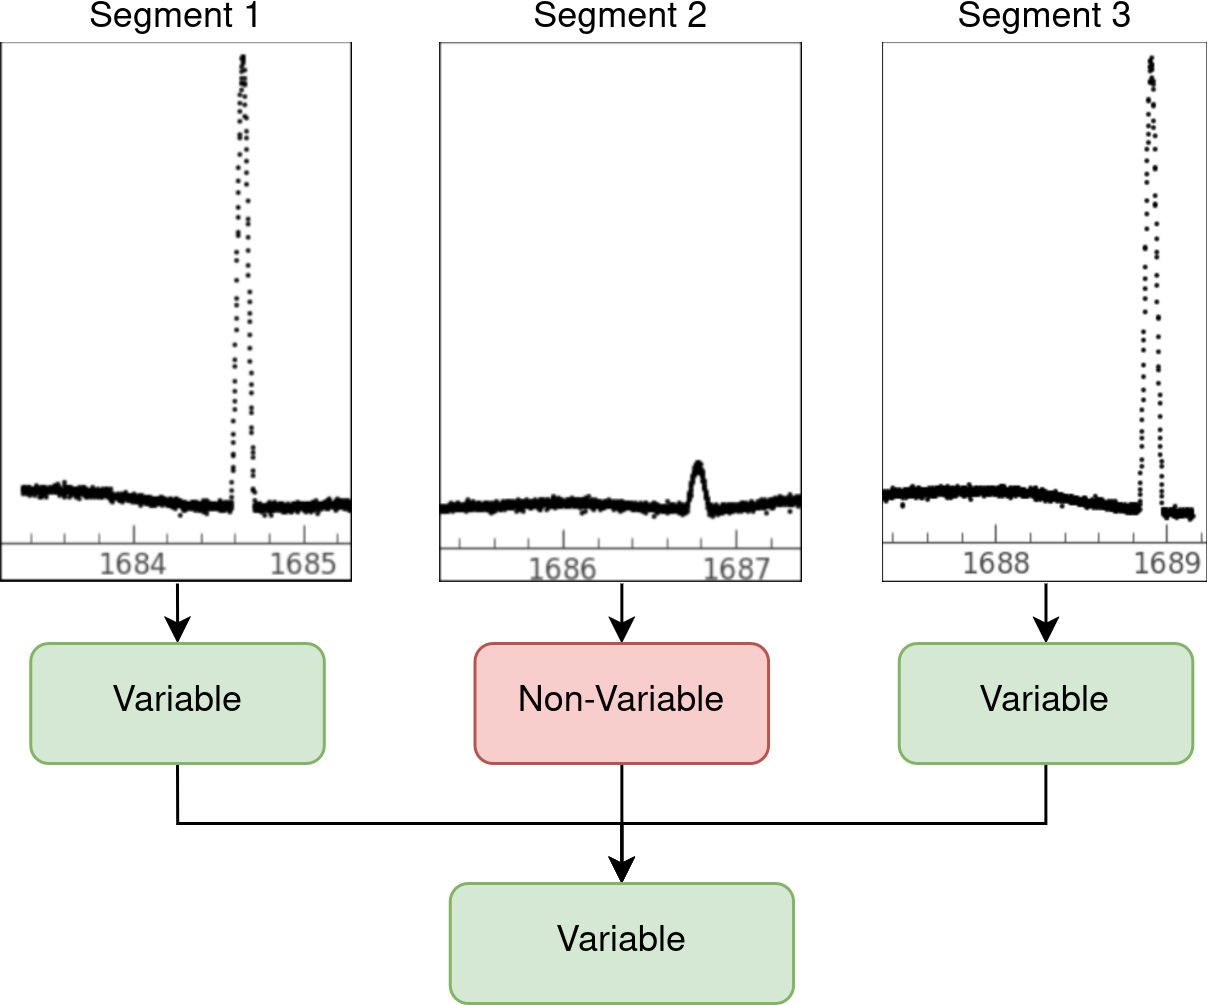
\includegraphics[width=0.8\linewidth]{images/06/segment_vs_tic_classification}
    \caption[Segment vs. TIC classification]{Comparison of segment-level and TIC-level classification - while one of the segments would individually misclassify the star, the final TIC-level prediction is correct. Note that the TIC-level prediction isn't done by majority voting, but rather by averaging logits.}
    \label{fig:06_segment_vs_tic_classification}
\end{figure}

\subsubsection{Segment \& Class Weighted Loss}\label{subsubsec:06-turbo-loss}

During training and validation, the loss was computed as a segment and class-weighted segment-level cross-entropy loss.
For a batch of segments, the model produces logits for each segment, and cross-entropy is computed independently for each one.
Class weights were applied inside the cross-entropy term to account for class imbalance.
To prevent TICs with many extracted segments from dominating, each segment was additionally weighted by the inverse of the number of segments belonging to its TIC.
Therefore, for segment $i$ from TIC $t$, the segment weight is

\[
    s_i = \frac{1}{n_t},
\]

where $n_t$ is the number of segments associated with TIC $t$.
The batch loss is then computed as the weighted average

\[
    \mathcal{L} = \frac{\sum_{i=1}^{B} s_i \, L_{\mathrm{WCE}}^{(i)}}{\sum_{i=1}^{B} s_i},
\]

where $B$ is the batch size and $L_{\mathrm{WCE}}^{(i)}$ is the \hyperref[eq:04-weighted-cross-entropy]{WeightedLoss} for segment $i$.

\bigskip

\noindent With this improvement, the training objective remained segment-based, but TIC-aware weighing ensured that each TIC contributed approximately equally to the loss.

\subsubsection{TIC-level Metrics}

The validation loss was computed at the end of each epoch using the same weighted segment-level cross-entropy objective as in training.

However, since we are interested in the model's performance on TIC level rather than the segment level, an additional TIC-level evaluation was performed during validation.

For each validation segment $i$ belonging to TIC $t$, the model output logits

\[
    \mathbf{z}_{t,i} = [z_{t,i,1}, z_{t,i,2}, \dots, z_{t,i,C}],
\]

where $C$ is the number of classes.
These logits were converted to class probabilities using the softmax function

\[
    p_{t,i,c} = \frac{\exp(z_{t,i,c})}{\sum_{k=1}^{C} \exp(z_{t,i,k})}.
\]

The class probabilities were then averaged over all $n_t$ segments belonging to the same TIC

\[
    \bar{p}_{t,c} = \frac{1}{n_t} \sum_{i=1}^{n_t} p_{t,i,c}.
\]

The predicted class for TIC $t$ was selected as the class with the highest mean probability

\[
    \hat{y}_t = \arg\max_{c} \bar{p}_{t,c}.
\]

Equivalently

\[
    \hat{y}_t = \arg\max_c \left(\frac{1}{n_t}\sum_{i=1}^{n_t}\mathrm{softmax}(\mathbf{z}_{t,i})_c\right).
\]

After aggregation, we obtained exactly one predicted label for each TIC.
TIC-level accuracy was then computed as

\[
    \mathrm{Accuracy}_{\mathrm{TIC}} = \frac{1}{T} \sum_{t=1}^{T} \mathbf{1}(\hat{y}_t = y_t),
\]

where $T$ is the number of TICs in the validation set and $y_t$ is the true class label of TIC $t$.

Other TIC-level metrics like Macro F1 were computed from the same aggregated TIC predictions.

\subsubsection{Best Model Selection}

The best model checkpoint was selected using the TIC-level mean-probability macro F1 score on the validation set.
This choice prioritizes performance on the final TIC-level classification task rather than on segment predictions.

Validation was therefore used for monitoring, plotting training curves, computing segment- and TIC-level metrics, and selecting the best checkpoint, it was however not used for gradient updates or direct optimization of the model parameters (that still relied on the weighted segment-level statistics).


\section{Model Architecture}

Our proposed architecture implements $5$ separate encoder-only transformer branches, one for each flux channel and one for the phase-folded channel, with a linear fusion layer behind them.
Additionally, scalar features are accessible through a small MLP branch.

Each of the 6 branches can be toggled on/off in the model config which allows for arbitrary combinations of the input channels.
Furthermore, the default PyTorch-based encoders in the transformer branches can be exchanged for pretrained transformer models and fine-tuned, further extending modularity of the system.

\begin{figure}[H]
    \centering
    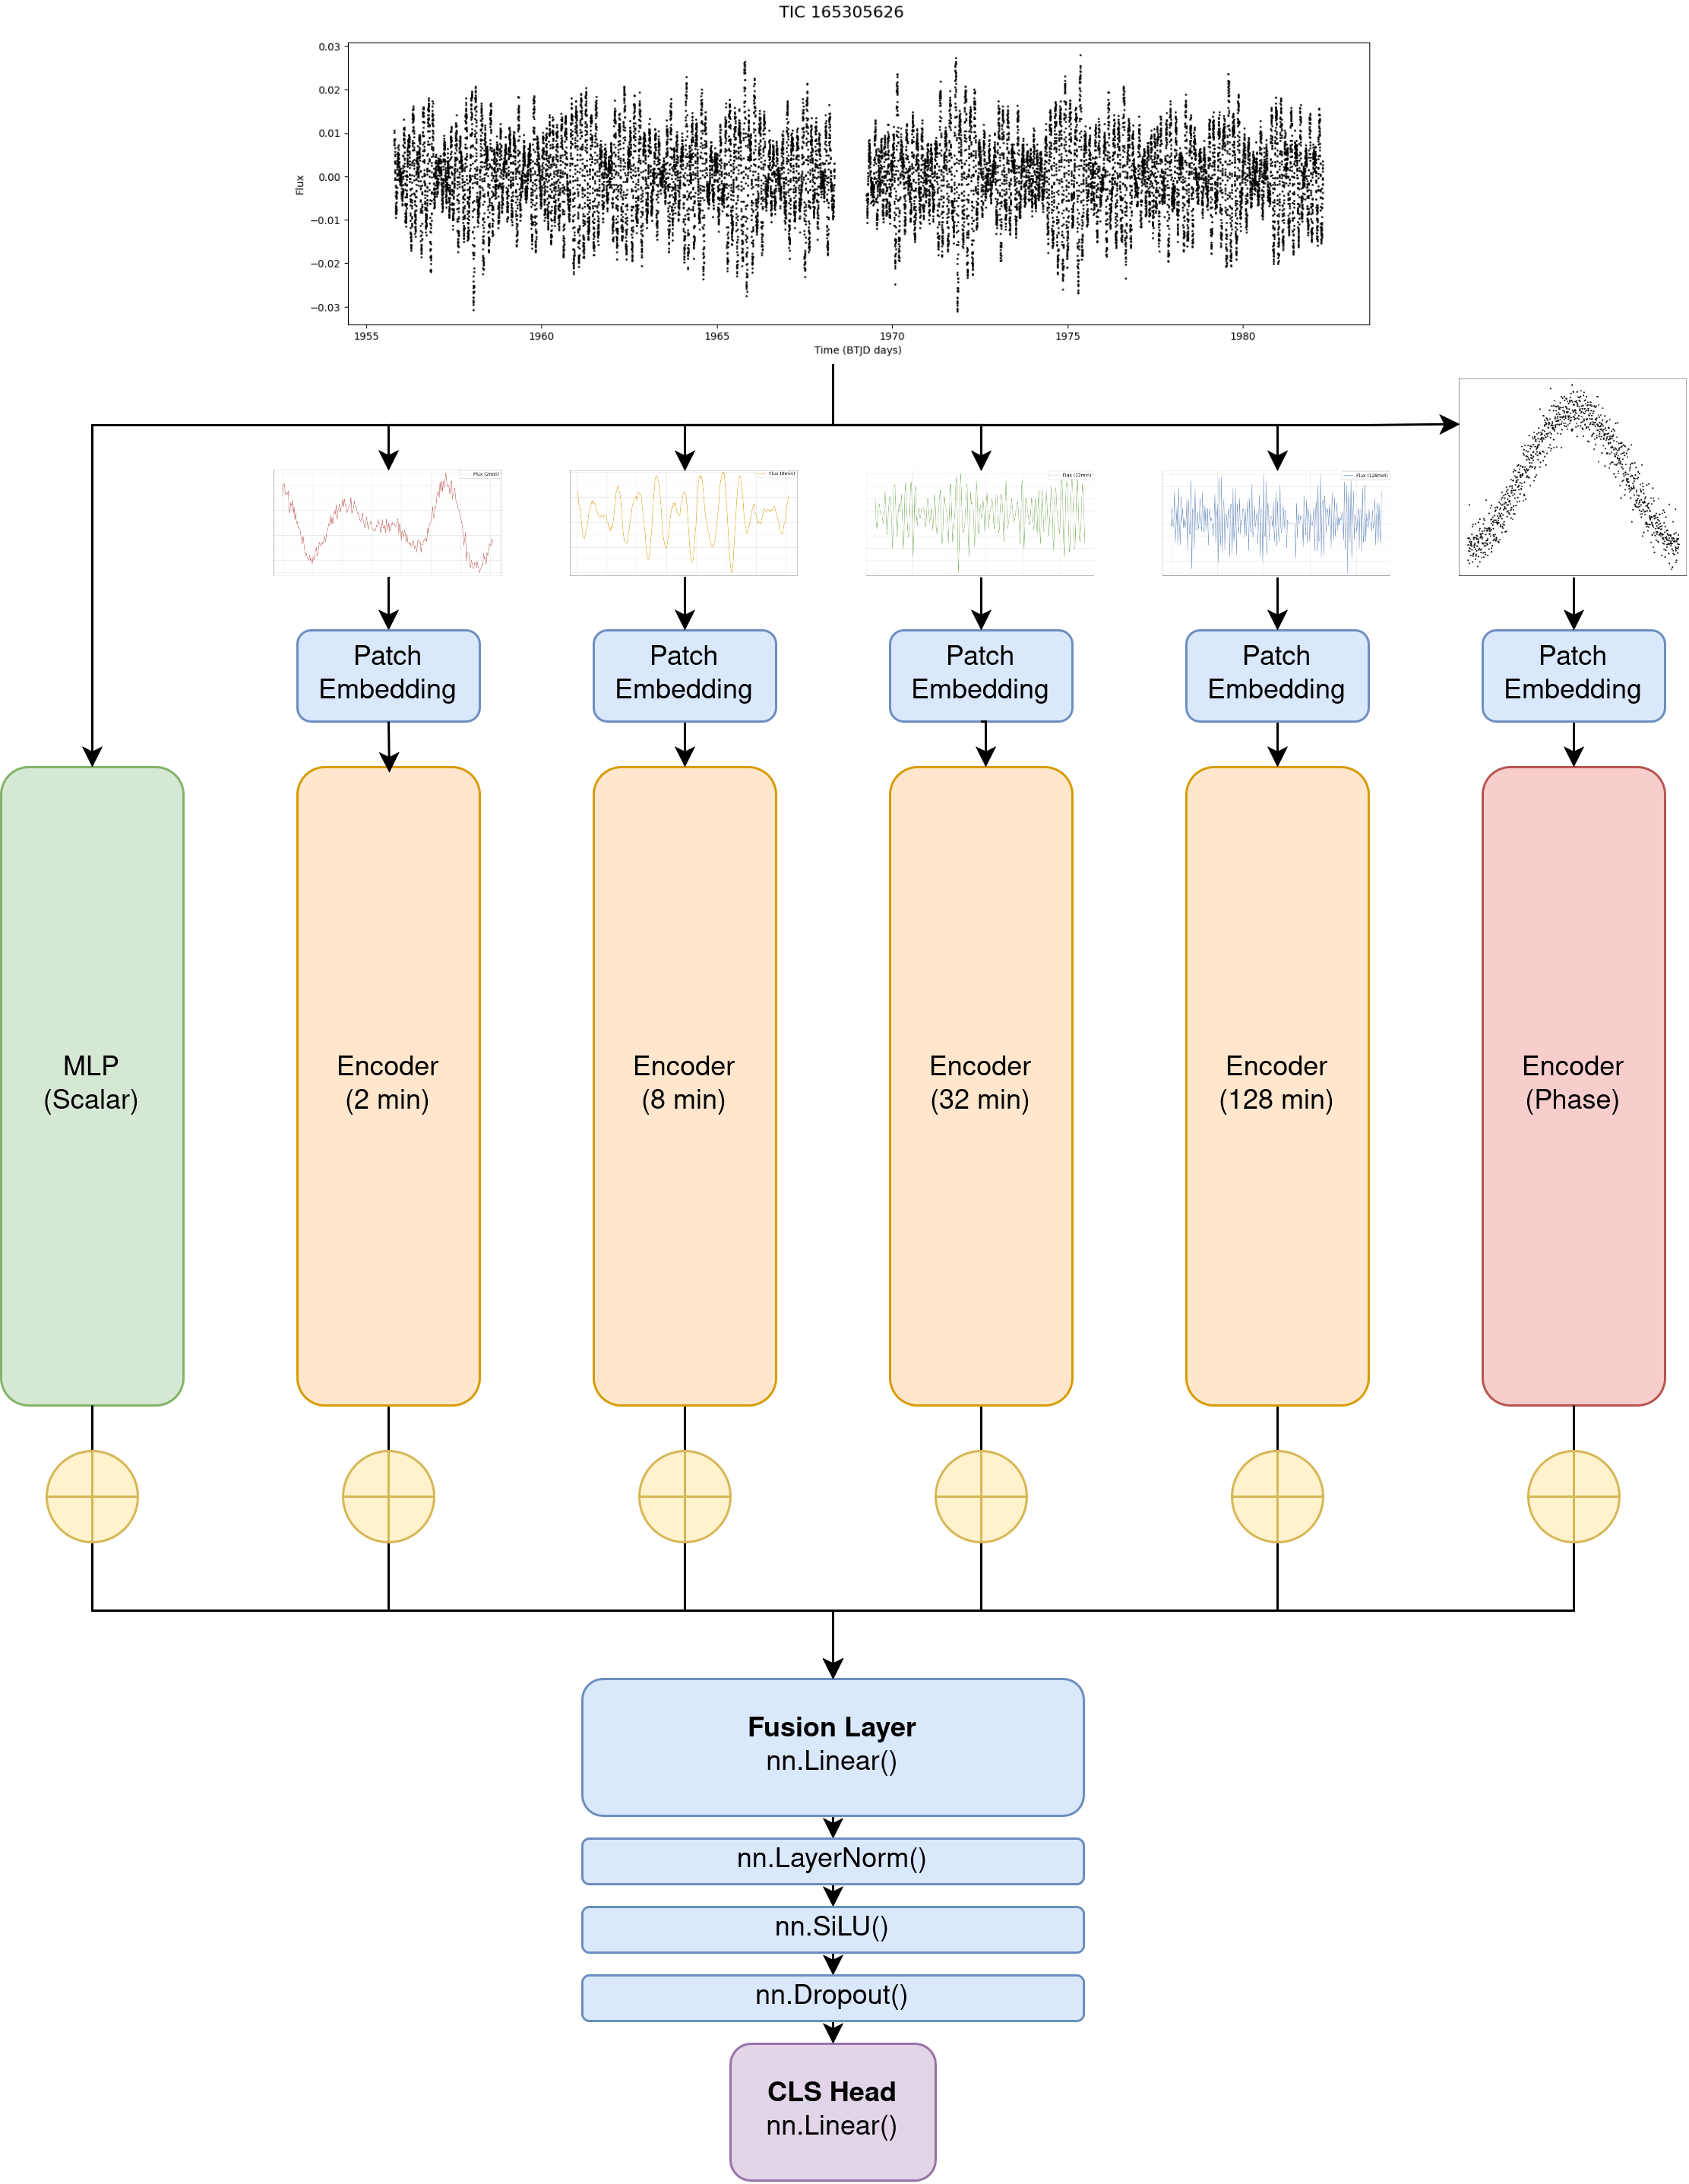
\includegraphics[width=\linewidth]{images/06/model_architecture}
    \caption[Model Architecture]{Proposed Model Architecture, each of the branches can be turned on/off separately, allowing arbitrary combinations of channels.}
    \label{fig:06_model_architecture}
\end{figure}

\FloatBarrier

\subsection{Embeddings}

We have experimented with two main types of embeddings:

\begin{itemize}
    \item \textbf{Learnable Embeddings.} While trivial to implement, they were prone to overfitting and didn't generalize as well.
    Another downside was the attention cost, since each data point turns into one token.
    \item \textbf{Patch Embeddings.} Similarly to \hyperref[subsec:04-base-transformer]{4.4.2 Base Transformer}, patch embeddings also performed really well on this task and were therefore used for most of the models.
\end{itemize}

\subsubsection{Statistical Patch Embeddings}

While even patch embeddings of raw flux values performed decently, we improved them by adding additional information computed from the patch.

For an input tensor of shape

\[
    (L, D)
\]

where $L$ is the sequence length and $D$ is the number of input channels ($\Phi$ and $\Phi_{\mathrm{err}}$), the tensor is reshaped into shape

\[
    (N, P, D)
\]

where $P$ is the selected patch size and $N = L / P$ is the number of resulting patches, to ensure divisibility by $P$, the sequence is padded as necessary.

For each patch, summary statistics are then computed, independently for each channel and using only valid positions according to the provided \hyperref[subsec:05-observation-gaps]{mask} to prevent invalid positions from influencing the result.

Specifically, the following features are computed for each patch $j$ and input channel $d$:

\begin{table}[H]
    \centering
    \small
    \renewcommand{\arraystretch}{1.3}
    \begin{tabularx}{\textwidth}{X c}
        \toprule
        \textbf{Parameter} & \textbf{Description} \tabularnewline
        \midrule
        $\mu_{j,d}$ & Mean \tabularnewline
        $\sigma_{j,d}$ & Standard Deviation \tabularnewline
        $\min_{j,d}$ & Minimum \tabularnewline
        $\max_{j,d}$ & Maximum \tabularnewline
        $m_{j,d}$ & Slope - approximated as $\frac{\mathrm{cov(input,time)}}{\mathrm{var(time)}}$ \tabularnewline
        $v$ & Fraction of valid points \tabularnewline
        \bottomrule
    \end{tabularx}
    \caption[Patch Statical Features]{Patch Statical Features}
    \label{tab:06_patch_statistical_featues}
\end{table}

The statistical features are then reshaped into vector of length $5D + 1$ (1~represents the valid point fraction), this vector is then projected into $d_{\mathrm{model}}$ using a compact 2 layer MLP.

The usage of statistical patch embeddings significantly improved the model performance by approximately $0.05 - 0.1 \Delta$ Macro F1.


\section{Implementation}

The implementation was again done in Python, with \textbf{PyTorch} and \textbf{Transformers} being the main libraries.
While initial prototyping was done using Jupyter notebooks, we decided to design and implement a modular framework that allows seamless running of different model configurations using only config files and minimal changes to the code.

\subsection{Structure}

The framework was developed as a self-contained python package:

\dirtree{%
    .1 /.
    .2 README.md \DTcomment{README file with documentation}.
    .2 \_\_main\_\_.py \DTcomment{Driver code}.
    .2 config.py \DTcomment{Experiment configuration}.
    .2 data.py \DTcomment{Dataset handling}.
    .2 evaluation.py \DTcomment{Metric computation}.
    .2 experiment.py \DTcomment{Experiment run orchestration}.
    .2 model.py \DTcomment{Implementation of the model components}.
    .2 trainer.py \DTcomment{Training run orchestration}.
    .2 utils.py \DTcomment{Utility and helper functions}.
}

\bigskip

The framework allows the user to setup the entire model configuration and training hyperparameters through a JSON configuration file.
Documentation and replicability of experiments if then trivial, since the original configuration file is saved alongside the results.
The framework also supports running multiple experiments sequentially in one run -- the driver code is only provided with a location of a directory that contains multiple configuration files and one experiment is then conducted for each of them.

Additionally, the trainer can continuously report the training progress to a Weights \& Biases\footnote{https://wandb.ai/} dashboard thas is accessible from the internet, allowing the user to remotely monitor long-running experiments.

\subsection{Saving Models}

Saving each model checkpoint quickly becomes memory intensive due to their large size, especially in the case of fine-tuned pretrained models.
To mitigate this issue, only one checkpoint was stored for each experiment.
This checkpoint was tracked by a custom callback triggered after each validation stage, TIC-level Macro F1 was computed and the tracked model was updated if improvement happened.

\subsection{Supported Transformer Architectures}

The framework allows configuration of the transformer architecture that is used in the transformer branches, the following architectures are supported

\begin{table}[H]
    \centering
    \footnotesize
    \renewcommand{\arraystretch}{1.3}
    \begin{tabularx}{\textwidth}{l c X}
        \toprule
        \textbf{Architecture} & \textbf{Type} & \textbf{Note} \tabularnewline
        \midrule
        Transformer & Transformer & The model is fully trained from scratch. \tabularnewline
        Chronos-2 & Pretrained TSFM\footnote{Time Series Foundation Model} & Accepts only raw flux values, handles tokenization and patching internally.  \tabularnewline
        Qwen 2.5 0.5B & Pretrained LLM & Largest model at around 1GB.   \tabularnewline
        \bottomrule
    \end{tabularx}
    \caption[Supported Transformer Architectures]{Supported Transformer Architectures}
    \label{tab:06_supported_transformer_architecture}
\end{table}

\subsubsection{Chronos-2}\label{subsubsec:06-chronos}

Chronos-2 is a 120M-parameter, encoder-only time series foundation model developed by Amazon.
While originally trained for time series forecasting, it can be fine-tuned for the classification task. \parencite{Ansari2025}


\section{Phase 1 -- Exploring Configurations}

In the first phase of experiments, various configurations of hyperparameters were tried to find a suitable baseline for further experiments.

\subsection{Patch Size}

\textbf{Patch Size} was one of the most influential parameters, multiple sizes from $4$ to $64$ were evaluated and $16$ was chosen as the best performing size.
Much larger and smaller values than $16$ performed significantly worse and either led to overfitting or did not converge reliably.

\subsection{Transformer Configuration}

The parameters for transformer configuration are intertwined with each other (for example, most publications recommend $d_{\mathrm{ff}} = 4 \cdot d_{\mathrm{model}}$).
Additionally, our experiments have shown that these parameters usually have some kind of \textbf{minimal viable value} -- models with lower values than the minimal viable value don't converge, however increasing it doesn't yield any further improvements.

The values that generally worked well for most configurations were:

\begin{table}[H]
    \centering
    \small
    \renewcommand{\arraystretch}{1.1}
    \begin{tabularx}{\textwidth}{X c}
        \toprule
        \textbf{Parameter} & \textbf{Value} \tabularnewline
        \midrule
        $n_{\mathrm{head}}$ & 8 \tabularnewline
        $n_{\mathrm{layers}}$ & 4 \tabularnewline
        $d_{\mathrm{model}}$ & 256 \tabularnewline
        $d_{\mathrm{ff}}$ & 1024 \tabularnewline
        $d_{\mathrm{fusion}}$ & 256 \tabularnewline
        \bottomrule
    \end{tabularx}
    \caption[Transformer Hyperparameters]{Transformer Hyperparameters}
    \label{tab:06_transformer_hyperparameters}
\end{table}

\subsection{Training}

Mutliple parameters for training were also explored:

\begin{itemize}
    \item \textbf{Learning Rate.} $5 \times 10^{-5}$ was chosen as a good baseline, since it achieved reliable convergence across most configurations.
    \item \textbf{Optimizer.} AdamW was chosen because it outperformed the simpler Adam optimizer.
    \item \textbf{Batch Size.} $64$ was at the upper limit of what could fit into the GPU VRAM, it also generally achieved slightly better validation performance than lower values.
    \item \textbf{Epochs.} $50$ was identified as a baseline, since it allowed most models to converge and show signs of overfitting at the end of the training.
    \item \textbf{Loss Function.} The proposed \hyperref[subsubsec:06-turbo-loss]{Segment \& Class Weighted Loss} was used.
\end{itemize}

\subsection{LR Scheduler}

Flat learning rate and multiple LR schedulers were tried, \textbf{CosineAnnealingLR} was then chosen due to its best performance.

The cosine annealing scheduler gradually decreases the learning rate $\eta$, following a cosine curve.

\[
    \eta_t = \eta_{\min} + \frac{1}{2}(\eta_{\max} - \eta_{\min})\left(1 + \cos\left(\pi \cdot \frac{t}{T_{\text{max}}}\right)\right)
\]

\begin{figure}[!htbp]
    \centering
    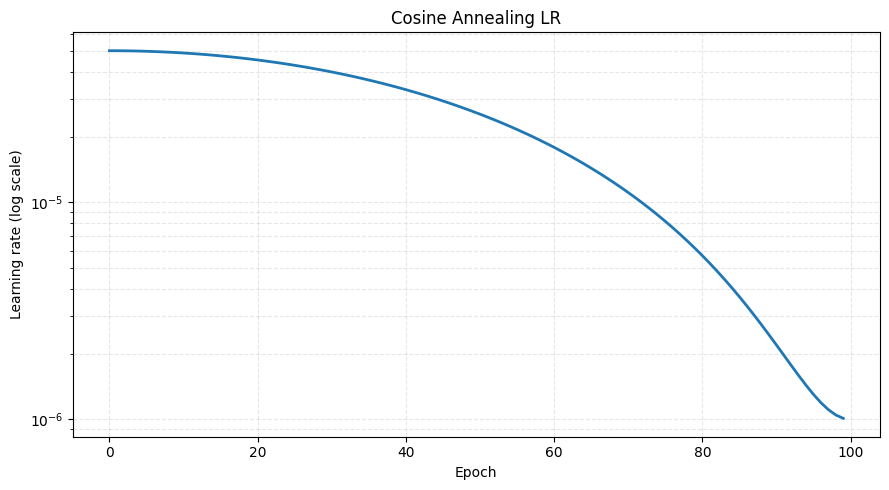
\includegraphics[width=0.6\linewidth]{images/06/cosine_annealing}
    \caption[Cosine Annealing LR]{Evolution of the learning rate, decreasing from $5 \times 10^{-5}$ to $1 \times 10^{-6}$}.
    \label{fig:06_cosine_annealing}
\end{figure}

\FloatBarrier

\subsection{Balanced Sampling}

This method was tried mainly on \textbf{Task B} due to the imbalanced dataset, however it limited the generalization of the model by over-predicting the eclipsing class.
It was therefore not used in future models.


\section{Phase 2 -- Basic Models}

Settings for a reasonably good baseline model were explored and identified in the previous phase.
In this phase, \textbf{12} experiments were conducted with a fixed set of hyperparameters, the only difference being the activated channels.

\begin{table}[H]
    \centering
    \small
    \renewcommand{\arraystretch}{1.1}
    \begin{tabularx}{\textwidth}{X c}
        \toprule
        \textbf{Parameter} & \textbf{Value} \tabularnewline
        \midrule
        Epochs & 50 \tabularnewline
        Learning Rate & 5 \times $10^{-5}$ \tabularnewline
        Batch Size & 64 \tabularnewline
        $n_{\mathrm{head}}$ & 8 \tabularnewline
        $n_{\mathrm{layers}}$ & 4 \tabularnewline
        $d_{\mathrm{model}}$ & 256 \tabularnewline
        $d_{\mathrm{ff}}$ & 1024 \tabularnewline
        $d_{\mathrm{fusion}}$ & 256 \tabularnewline
        Patch Size & 16 \tabularnewline
        Dropout & 0.15 \tabularnewline
        Loss & WeightedLoss \tabularnewline
        Optimizer & AdamW \tabularnewline
        Weight Decay & 1 \times $10^{-2}$ \tabularnewline
        \bottomrule
    \end{tabularx}
    \caption[Phase 2 Hyperparameters]{Phase 2 Hyperparameters}
    \label{tab:06_phase_2_hyperparameters}
\end{table}

\subsection{1-Channel Transformers}

Initially, only $1$ of the $4$ available flux sequence channels was selected at a time.

\subsubsection{Task A}

The training took around $20$ minutes for each of the models.

\begin{table}[H]
    \centering
    \small
    \renewcommand{\arraystretch}{1.1}
    \begin{tabularx}{\textwidth}{X c c c c}
        \toprule
        \textbf{Channel} & \textbf{Accuracy} & \textbf{Macro F1} & \textbf{TIC Accuracy} & \textbf{TIC Macro F1}  \tabularnewline
        \midrule
        2-min & 0.72 & 0.72 & 0.84 & 0.84 \tabularnewline
        8-min & 0.78 & 0.78 & 0.87 & 0.87 \tabularnewline
        32-min & 0.80 & 0.80 & 0.87 & 0.87 \tabularnewline
        128-min & 0.77 & 0.77 & 0.84 & 0.84 \tabularnewline
        \bottomrule
    \end{tabularx}
    \caption[Phase 2 -- 1-Channel Transformer Metrics (A)]{1-Channel Transformer Validation Metrics (Task A)}
    \label{tab:06_phase_2_1_channel_a}
\end{table}

\FloatBarrier

The 32-min channel performed the best, it was therefore selected for further evaluation.

\begin{figure}[!htbp]
    \centering
    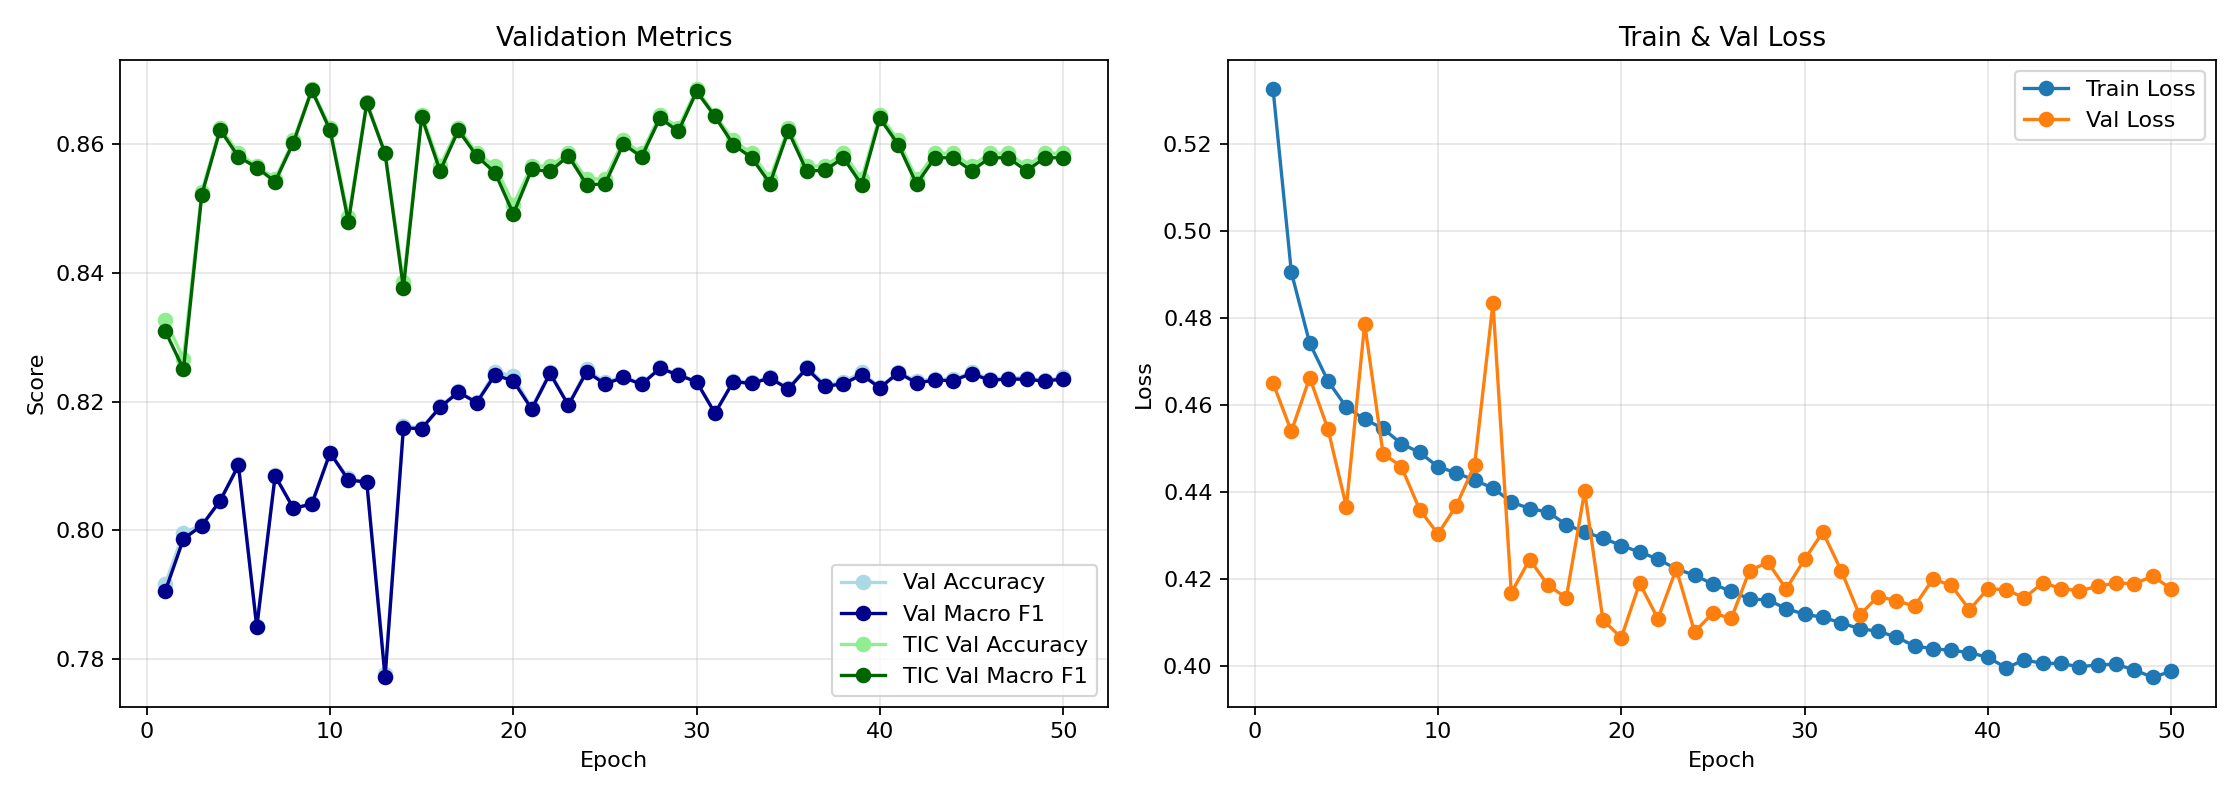
\includegraphics[width=\linewidth]{images/06/phase2_A_1c_training_curves}
    \caption[Phase 2 -- 32-min Channel Transformer Training Curves (A)]{32-min Channel Transformer Training Curves (Task A)}
    \label{fig:06_phase_2_32_min_channel_transformer_training_curves_a}
\end{figure}

\FloatBarrier

The training loss steadily continued to decrease throughout the training, the validation loss also decrease until around epoch $25$, although it was much more unstable.
After epoch $25$, the model probably started overfitting.

It should be noted the disparity between segment-level and TIC-level metrics ($\Delta \approx 0.04$) throughout the entire training, the segment logit aggregation seems to work really well for blabel prediction of individual stars.

\begin{table}[H]
    \centering
    \footnotesize
    \renewcommand{\arraystretch}{1.1}

    \begin{minipage}[t]{0.32\textwidth}
        \centering
        \begin{tabularx}{\textwidth}{X c}
            \toprule
            \textbf{Metric} & \textbf{Score} \tabularnewline
            \midrule
            Accuracy    &  0.8041 \tabularnewline
            Macro F1    & 0.8041 \tabularnewline
            TIC Accuracy & 0.8685 \tabularnewline
            TIC Macro F1 & 0.8636 \tabularnewline
            \bottomrule
        \end{tabularx}
    \end{minipage}
    \hfill
    \begin{minipage}[t]{0.64\textwidth}
        \centering
        \footnotesize
        \begin{tabularx}{\textwidth}{X c c c c c}
            \toprule
            \textbf{Class} & \textbf{Precision} & \textbf{Recall} & \textbf{F1-score} & \textbf{Support} \tabularnewline
            \midrule
            N & 0.87 & 0.88 & 0.87 & 259 \tabularnewline
            V & 0.87 & 0.86 & 0.86 & 243   \tabularnewline
            \bottomrule
        \end{tabularx}
    \end{minipage}

    \caption[Phase 2 -- 32-min Transformer Validation Metrics (A)]{Validation Metrics (Task A)}
    \label{tab:06_phase_2_32_min_channel_transformer_validation_,etrics_a}
\end{table}

\FloatBarrier

The validation predictions for both classes were balanced, none of them was visibly preferred.

\subsubsection{Task B}

The training took around $5$ minutes for each of the models, which is proportional to the difference of sizes between the two datasets.

\begin{table}[H]
    \centering
    \small
    \renewcommand{\arraystretch}{1.1}
    \begin{tabularx}{\textwidth}{X c c c c}
        \toprule
        \textbf{Channel} & \textbf{Accuracy} & \textbf{Macro F1} & \textbf{TIC Accuracy} & \textbf{TIC Macro F1}  \tabularnewline
        \midrule
        2-min & 0.66 & 0.59 & 0.72 & 0.69 \tabularnewline
        8-min & 0.77 & 0.72 & 0.86 & 0.82 \tabularnewline
        32-min & 0.83 & 0.81 & 0.87 & 0.86 \tabularnewline
        128-min & 0.88 & 0.88 & 0.90 & 0.91 \tabularnewline
        \bottomrule
    \end{tabularx}
    \caption[Phase 2 -- 1-Channel Transformer Metrics (B)]{1-Channel Transformer Validation Metrics (Task B)}
    \label{tab:06_phase_2_1_channel_b}
\end{table}

\FloatBarrier

The 128-min channel performed the best, it was therefore chosen for further evaluation.

\begin{figure}[!htbp]
    \centering
    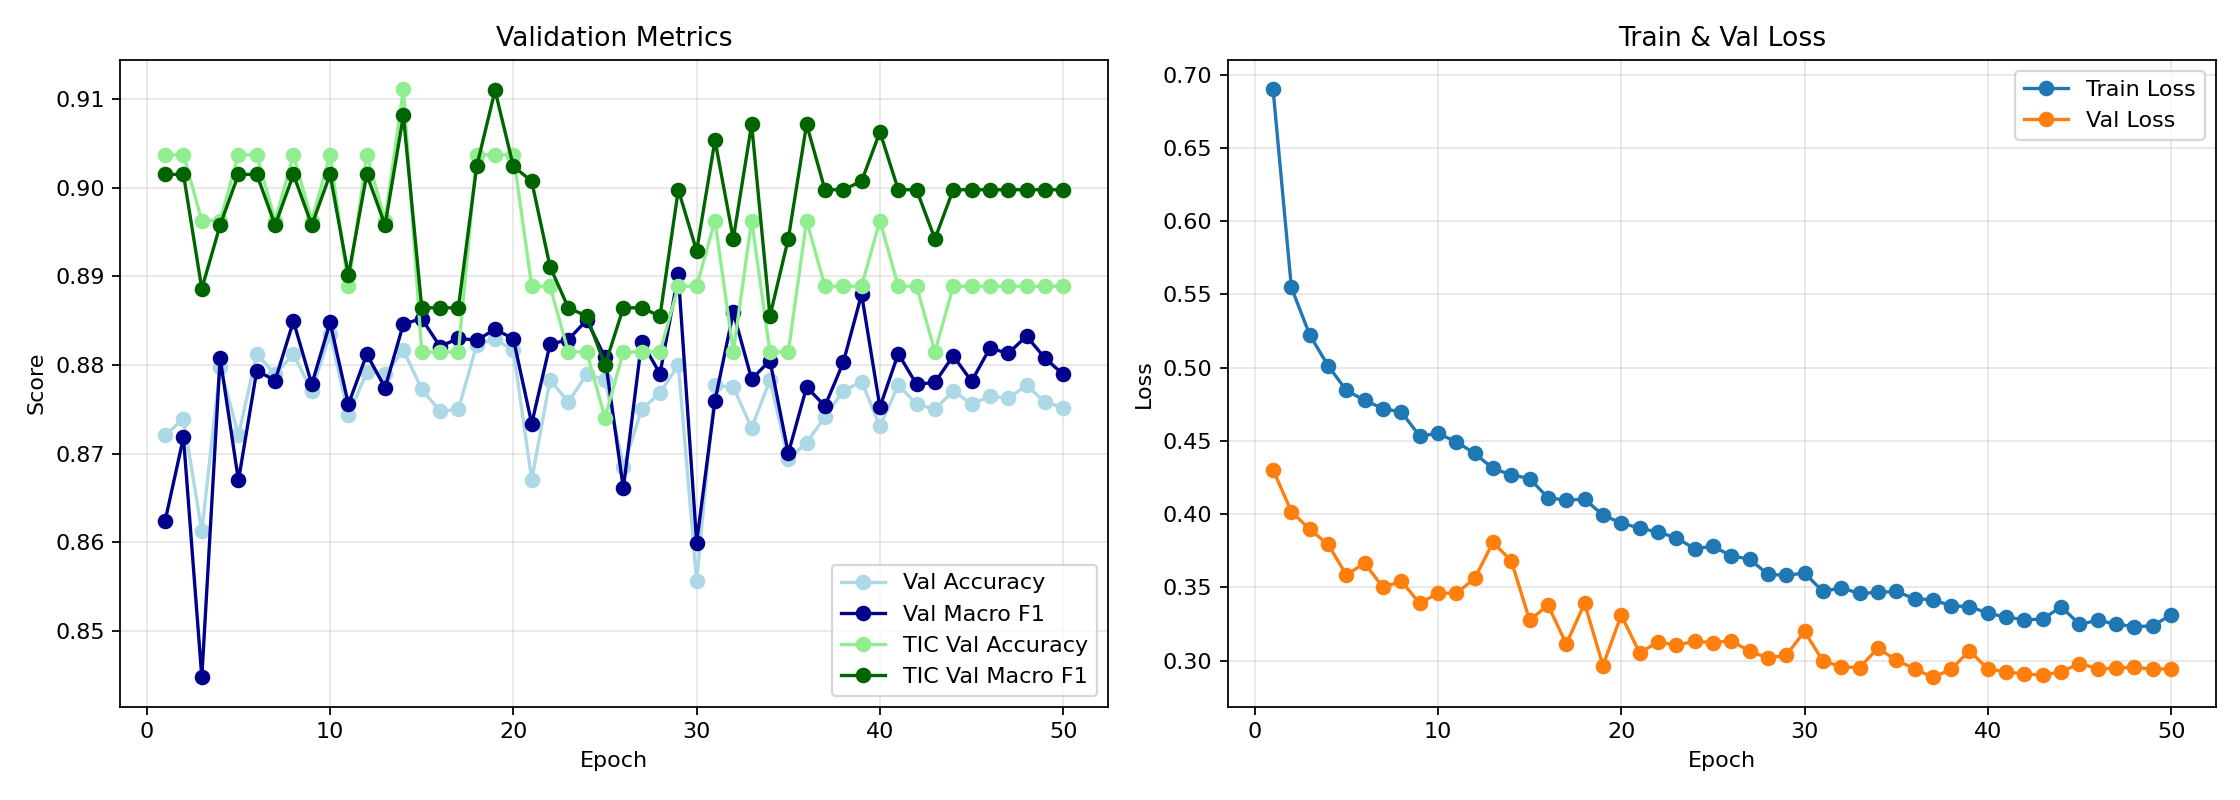
\includegraphics[width=\linewidth]{images/06/phase2_B_1c_training_curves}
    \caption[Phase 2 -- 128-min Channel Transformer Training Curves (B)]{128-min Channel Transformer Training Curves (Task B)}
    \label{fig:06_phase_2_128_min_channel_transformer_training_curves_b}
\end{figure}

\FloatBarrier

While the training loss continued to decrease, the validation loss went down and stagnated at around $0.3$.
The model was probably too simple to overfit and would've benefitted from more parameters.

The TIC-level aggregated predictions were again significantly better than raw segment-level predictions.

\begin{table}[H]
    \centering
    \footnotesize
    \renewcommand{\arraystretch}{1.1}

    \begin{minipage}[t]{0.32\textwidth}
        \centering
        \begin{tabularx}{\textwidth}{X c}
            \toprule
            \textbf{Metric} & \textbf{Score} \tabularnewline
            \midrule
            Accuracy    &  0.8829 \tabularnewline
            Macro F1    & 0.8840 \tabularnewline
            TIC Accuracy & 0.9037 \tabularnewline
            TIC Macro F1 & 0.9110 \tabularnewline
            \bottomrule
        \end{tabularx}
    \end{minipage}
    \hfill
    \begin{minipage}[t]{0.64\textwidth}
        \centering
        \footnotesize
        \begin{tabularx}{\textwidth}{X c c c c c}
            \toprule
            \textbf{Class} & \textbf{Precision} & \textbf{Recall} & \textbf{F1-score} & \textbf{Support} \tabularnewline
            \midrule
            E & 1.00 & 0.93 & 0.97 & 15 \tabularnewline
            P & 0.95 & 0.90 & 0.92 & 81   \tabularnewline
            R & 0.80 & 0.90 & 0.84 & 39 \tabularnewline
            \bottomrule
        \end{tabularx}
    \end{minipage}

    \caption[Phase 2 -- 128-min Transformer Validation Metrics (B)]{Validation Metrics (Task B)}
    \label{tab:06_phase_2_128_min_channel_transformer_validation_,etrics_b}
\end{table}

The model performed really well on the \textbf{eclipsing} class, which may seem surprising, because it's the class with the lowest sample count.
However, the light curves of eclipsing stars are the most recognizable with sharp peaks that are strongly periodic.
Although it good also be caused by random chance, since even one additional (un)successful classification can heavily skew the Macro F1 score.

\subsection{Multi-Channel Transformers}

After the single-channel baseline models, two additional configurations were evaluated - one with all 6 channels\footnote{Only 5 of those channels utilize the transformer architecture -- the 6th channel consists of scalar features that are handled by a non-transformer MLP.} enabled and one with only the 4 flux channels enabled (no phase-folded information).

The training took around $50$ minutes for the smaller model and around $70$ for the larger one on Task A and was proportionally shorter on Task B\@.

\subsubsection{Task A}

\begin{table}[H]
    \centering
    \small
    \renewcommand{\arraystretch}{1.1}
    \begin{tabularx}{\textwidth}{X c c c c}
        \toprule
        \textbf{Configuration} & \textbf{Accuracy} & \textbf{Macro F1} & \textbf{TIC Accuracy} & \textbf{TIC Macro F1}  \tabularnewline
        \midrule
        4-channel & 0.85 & 0.85 & 0.90 & 0.90 \tabularnewline
        6-channel & 0.88 & 0.88 & 0.91 & 0.91 \tabularnewline
        \bottomrule
    \end{tabularx}
    \caption[Phase 2 -- Multi-Channel Transformer Metrics (A)]{Multi-Channel Transformer Validation Metrics (Task A)}
    \label{tab:06_phase_2_multi_channel_a}
\end{table}

\FloatBarrier

The 6-channel model performed better, it was therefore selected for further evaluation.

\begin{figure}[!htbp]
    \centering
    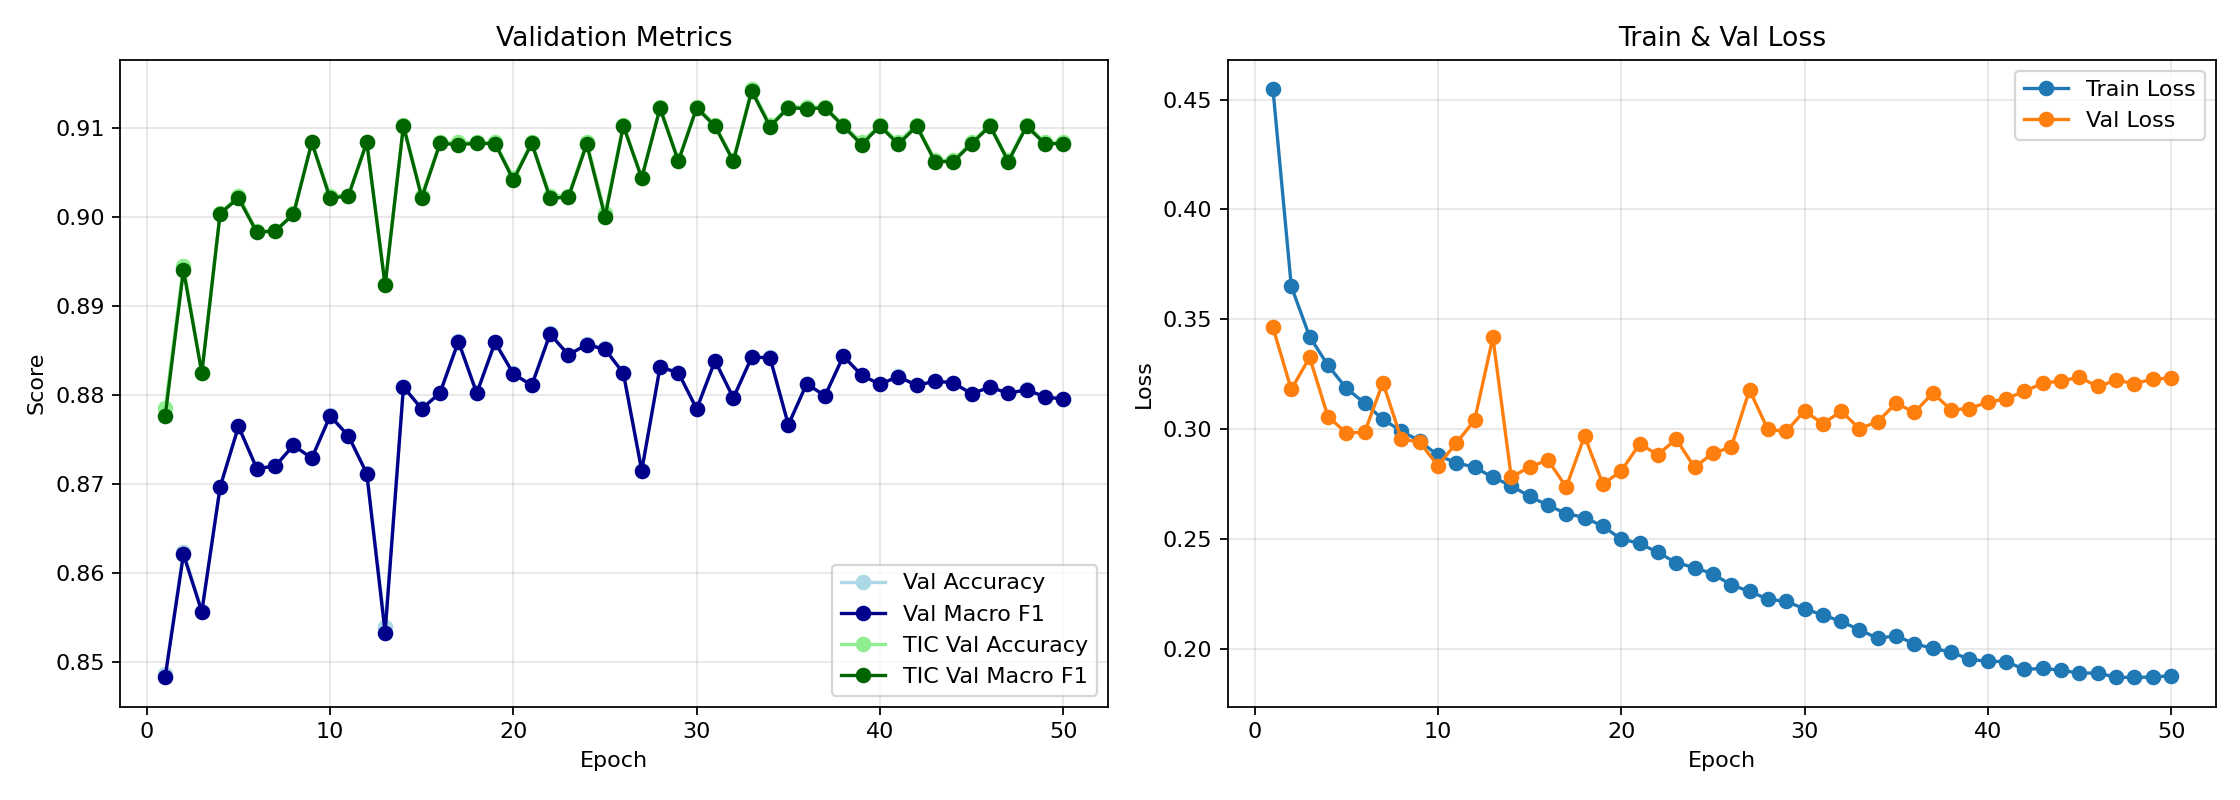
\includegraphics[width=\linewidth]{images/06/phase2_A_6c_training_curves}
    \caption[Phase 2 -- 6-Channel Transformer Training Curves (A)]{6-Channel Transformer Training Curves (Task A)}
    \label{fig:06_phase_2_6_channel_transformer_training_curves_a}
\end{figure}

\FloatBarrier

The training loss continued to decrease and diverged from the validation loss at around epoch $20$, TIC-level Macro F1 stagnated while segment-level Macro F1 continued to decrease as the model probably overfitted.

\begin{table}[H]
    \centering
    \footnotesize
    \renewcommand{\arraystretch}{1.1}

    \begin{minipage}[t]{0.32\textwidth}
        \centering
        \begin{tabularx}{\textwidth}{X c}
            \toprule
            \textbf{Metric} & \textbf{Score} \tabularnewline
            \midrule
            Accuracy    &  0.8527 \tabularnewline
            Macro F1    & 0.8527 \tabularnewline
            TIC Accuracy & 0.8984 \tabularnewline
            TIC Macro F1 & 0.8983 \tabularnewline
            \bottomrule
        \end{tabularx}
    \end{minipage}
    \hfill
    \begin{minipage}[t]{0.64\textwidth}
        \centering
        \footnotesize
        \begin{tabularx}{\textwidth}{X c c c c c}
            \toprule
            \textbf{Class} & \textbf{Precision} & \textbf{Recall} & \textbf{F1-score} & \textbf{Support} \tabularnewline
            \midrule
            N & 0.91 & 0.90 & 0.90 & 259 \tabularnewline
            V & 0.89 & 0.90 & 0.90 & 243   \tabularnewline
            \bottomrule
        \end{tabularx}
    \end{minipage}

    \caption[Phase 2 -- 6-Channel Transformer Validation Metrics (A)]{Validation Metrics (Task A)}
    \label{tab:06_phase_2_6_channel_transformer_validation_,etrics_a}
\end{table}

\FloatBarrier

The validation predictions for both classes were again balanced.

\subsubsection{Task B}

\begin{table}[H]
    \centering
    \small
    \renewcommand{\arraystretch}{1.1}
    \begin{tabularx}{\textwidth}{X c c c c}
        \toprule
        \textbf{Configuration} & \textbf{Accuracy} & \textbf{Macro F1} & \textbf{TIC Accuracy} & \textbf{TIC Macro F1}  \tabularnewline
        \midrule
        4-channel & 0.87 & 0.88 & 0.92 & 0.92 \tabularnewline
        6-channel & 0.89 & 0.89 & 0.92 & 0.92 \tabularnewline
        \bottomrule
    \end{tabularx}
    \caption[Phase 2 -- 1-Channel Transformer Metrics (B)]{1-Channel Transformer Validation Metrics (Task B)}
    \label{tab:06_phase_2_1_channel_bx}
\end{table}

\FloatBarrier

The 6-channel model again outperformed the 4-channel, although almost negligibly.

\begin{figure}[!htbp]
    \centering
    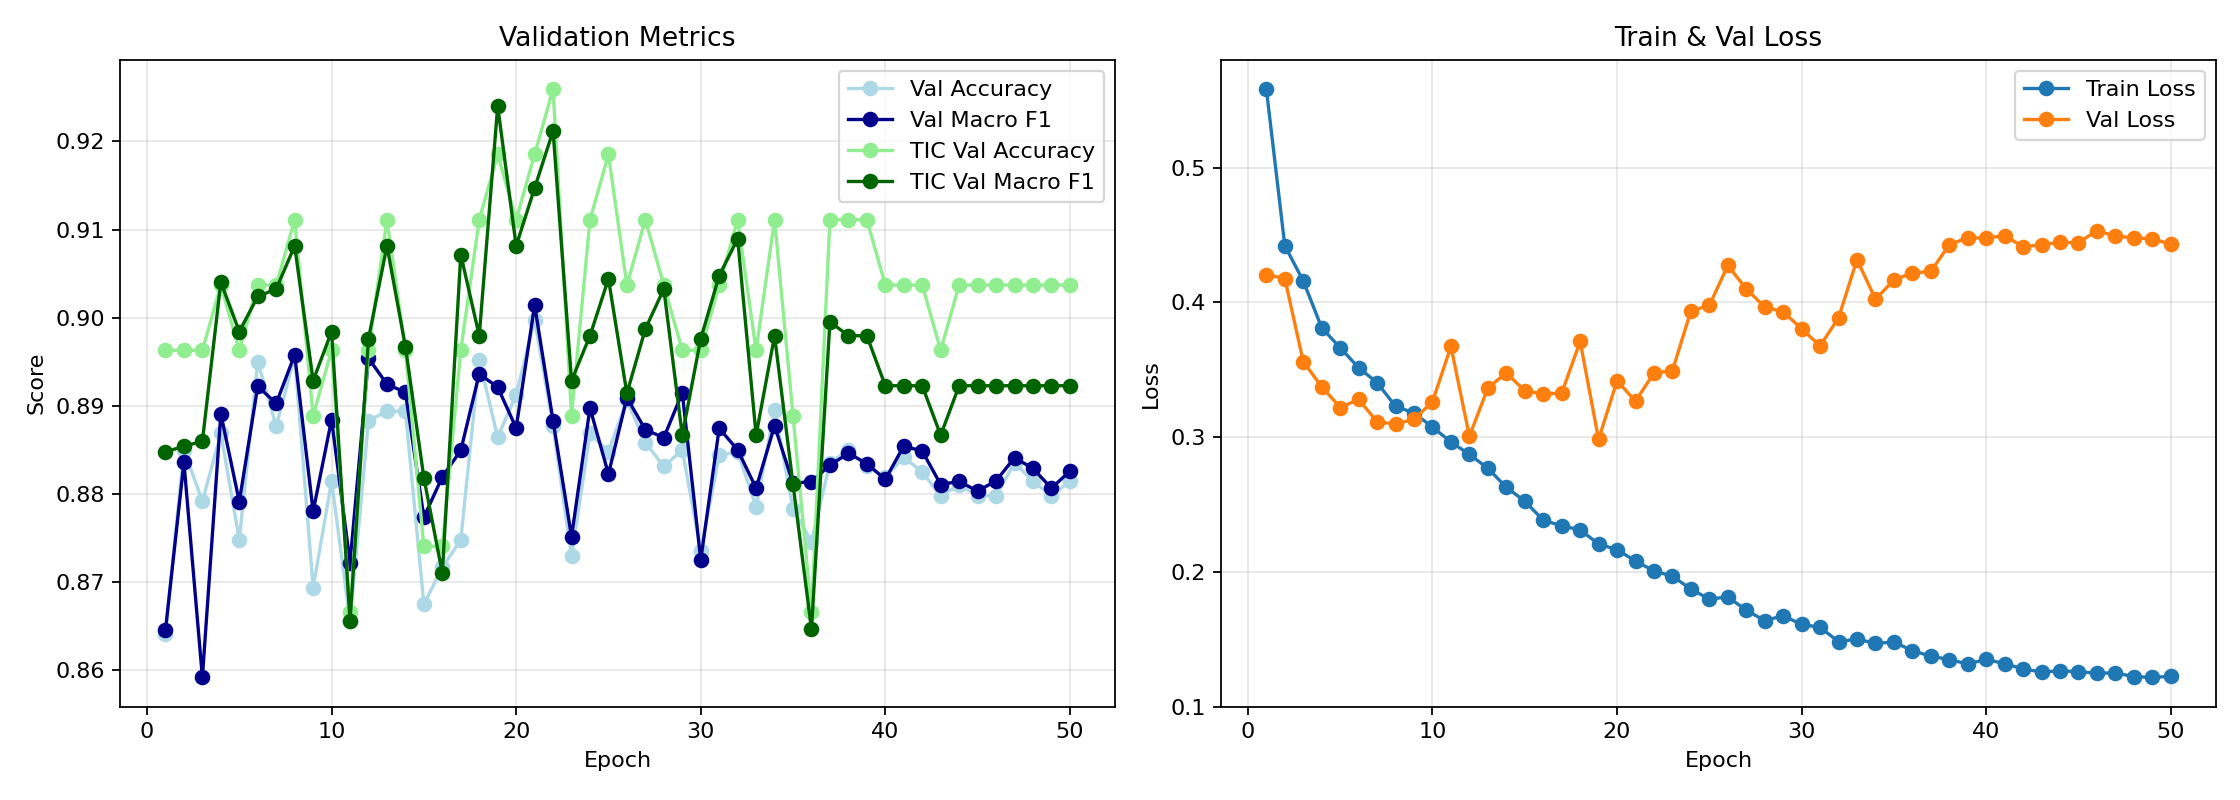
\includegraphics[width=\linewidth]{images/06/phase2_B_6c_training_curves}
    \caption[Phase 2 -- 6-Channel Transformer Training Curves (B)]{6-Channel Transformer Training Curves (Task B)}
    \label{fig:06_phase_2_6_channel_transformer_training_curves_b}
\end{figure}

\FloatBarrier

The training loss decreased steadily and diverged from the validation loss quite early, after epoch $10$, validation metrics showed unstable behavior throughout the whole training.

\begin{table}[H]
    \centering
    \footnotesize
    \renewcommand{\arraystretch}{1.1}

    \begin{minipage}[t]{0.32\textwidth}
        \centering
        \begin{tabularx}{\textwidth}{X c}
            \toprule
            \textbf{Metric} & \textbf{Score} \tabularnewline
            \midrule
            Accuracy    &  0.8867 \tabularnewline
            Macro F1    & 0.8921 \tabularnewline
            TIC Accuracy & 0.9185 \tabularnewline
            TIC Macro F1 & 0.9240 \tabularnewline
            \bottomrule
        \end{tabularx}
    \end{minipage}
    \hfill
    \begin{minipage}[t]{0.64\textwidth}
        \centering
        \footnotesize
        \begin{tabularx}{\textwidth}{X c c c c c}
            \toprule
            \textbf{Class} & \textbf{Precision} & \textbf{Recall} & \textbf{F1-score} & \textbf{Support} \tabularnewline
            \midrule
            E & 1.00 & 0.93 & 0.97 & 15 \tabularnewline
            P & 0.97 & 0.90 & 0.94 & 81   \tabularnewline
            R & 0.80 & 0.95 & 0.87 & 39 \tabularnewline
            \bottomrule
        \end{tabularx}
    \end{minipage}

    \caption[Phase 2 -- 6-Channel Transformer Validation Metrics (B)]{Validation Metrics (Task B)}
    \label{tab:06_phase_2_6_channel_transformer_validation_,etrics_b}
\end{table}

The model has shown great classification performance for all of the classes, however it may not be able to generalize well due to strong signs of overfitting from the training metrics.


\section{Phase 3 -- Pretrained Model Fine-Tuning}

In this phase, $2$ different pretrained models were fined-tuned:

\begin{itemize}
    \item \textbf{Chronos-2.} A 120M parameter pretrained TSFM, originally trained for time series forecasting.
    \item \textbf{Qwen 2.5 0.5B.} A 500M parameter pretrained LLM, designed for text completion.
\end{itemize}

We have decided to not utilize pretrained vision transformers in our experiments, mainly because we believe the task is fundamentally 1-dimensional at the physical level.

Both fine-tunes were performed with \hyperref[subsubsec:03-lora]{LoRA} (the original model weights remained frozen), the following parameters were used:

\begin{table}[H]
    \centering
    \small
    \renewcommand{\arraystretch}{1.1}
    \begin{tabularx}{\textwidth}{X c}
        \toprule
        \textbf{Parameter} & \textbf{Value} \tabularnewline
        \midrule
        Epochs & 10 \tabularnewline
        Learning Rate & 5 \times $10^{-5}$ \tabularnewline
        LoRA $r$ & 8 \tabularnewline
        LoRA $\alpha$ & 16 \tabularnewline
        Batch Size & 64 (32 for Qwen) \tabularnewline
        Patch Size & 16 (Chronos-2 expects the raw flux) \tabularnewline
        Dropout & 0.15 \tabularnewline
        Loss & WeightedLoss \tabularnewline
        Optimizer & AdamW \tabularnewline
        Weight Decay & 1 \times $10^{-2}$ \tabularnewline
        \bottomrule
    \end{tabularx}
    \caption[Phase 2 Hyperparameters]{Phase 2 Hyperparameters}
    \label{tab:06_phase_3_hyperparameters}
\end{table}

Both models were trained on all 6 available channels, batch size needed to be reduced for Qwen due to memory constraints.

The number of epochs was also reduced, because the fine-tuning of pretraining generally takes significantly less training steps compared to training from scratch.
However, because the pretrained models are much larger than the original transformers, the training can still take significant amounts of time.

\subsection{Chronos-2}

The training took around $100$ and $30$ minutes for tasks A and B respectively.

\subsubsection{Task A}

\begin{figure}[!htbp]
    \centering
    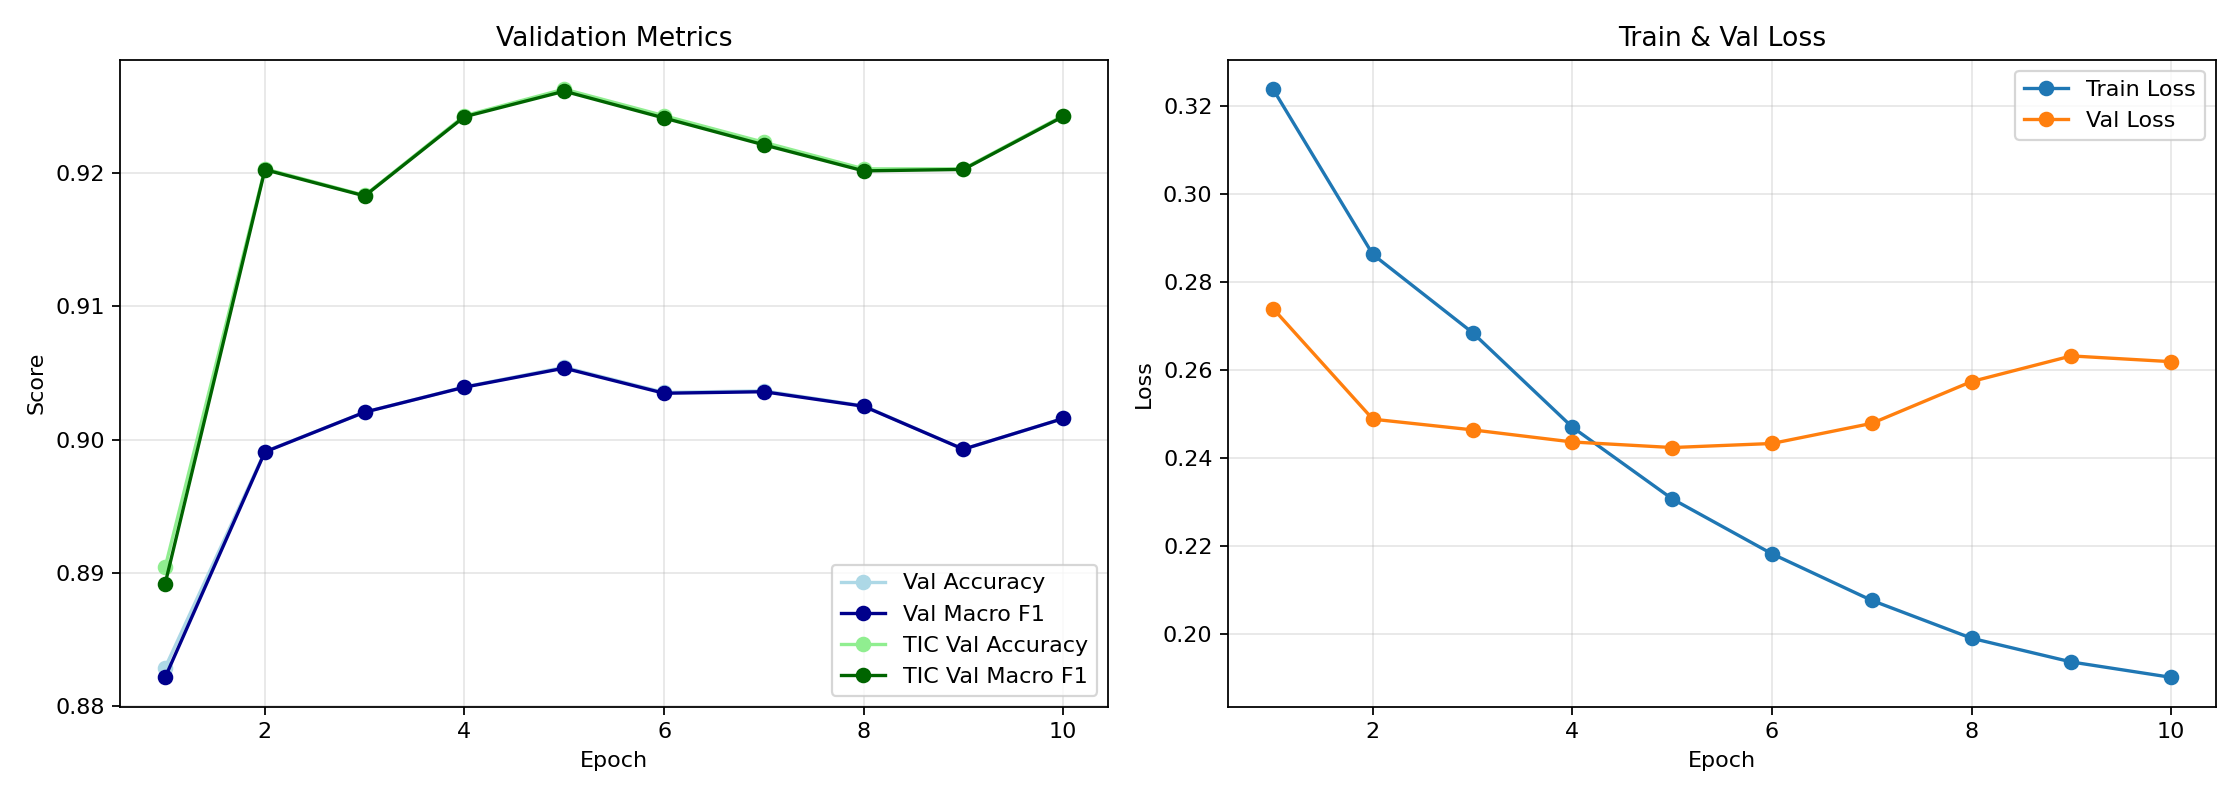
\includegraphics[width=\linewidth]{images/06/phase3_A_chronos_training_curves}
    \caption[Phase 3 -- Chronos-2 Training Curves (A)]{Chronos-2 Training Curves (Task A)}
    \label{fig:06_phase_3_chronos_training_curves_A}
\end{figure}

\FloatBarrier

The training loss steadily decreased and diverged from the validation loss at around epoch $4$, the best TIC Val Macro F1 was observed at epoch $5$.

\begin{table}[H]
    \centering
    \footnotesize
    \renewcommand{\arraystretch}{1.1}

    \begin{minipage}[t]{0.32\textwidth}
        \centering
        \begin{tabularx}{\textwidth}{X c}
            \toprule
            \textbf{Metric} & \textbf{Score} \tabularnewline
            \midrule
            Accuracy    &  0.9054 \tabularnewline
            Macro F1    & 0.9054 \tabularnewline
            TIC Accuracy & 0.9263 \tabularnewline
            TIC Macro F1 & 0.9261 \tabularnewline
            \bottomrule
        \end{tabularx}
    \end{minipage}
    \hfill
    \begin{minipage}[t]{0.64\textwidth}
        \centering
        \footnotesize
        \begin{tabularx}{\textwidth}{X c c c c c}
            \toprule
            \textbf{Class} & \textbf{Precision} & \textbf{Recall} & \textbf{F1-score} & \textbf{Support} \tabularnewline
            \midrule
            N & 0.92 & 0.94 & 0.93 & 259 \tabularnewline
            V & 0.93 & 0.91 & 0.92 & 243   \tabularnewline
            \bottomrule
        \end{tabularx}
    \end{minipage}

    \caption[Phase 3 -- Chronos-2 Validation Metrics (A)]{Validation Metrics (Task A)}
    \label{tab:06_phase_3_chronos_validation_,etrics_A}
\end{table}

\FloatBarrier

The validation predictions were a notable improvement over the previous best 6-channel transformer.

\subsubsection{Task B}

\begin{figure}[!htbp]
    \centering
    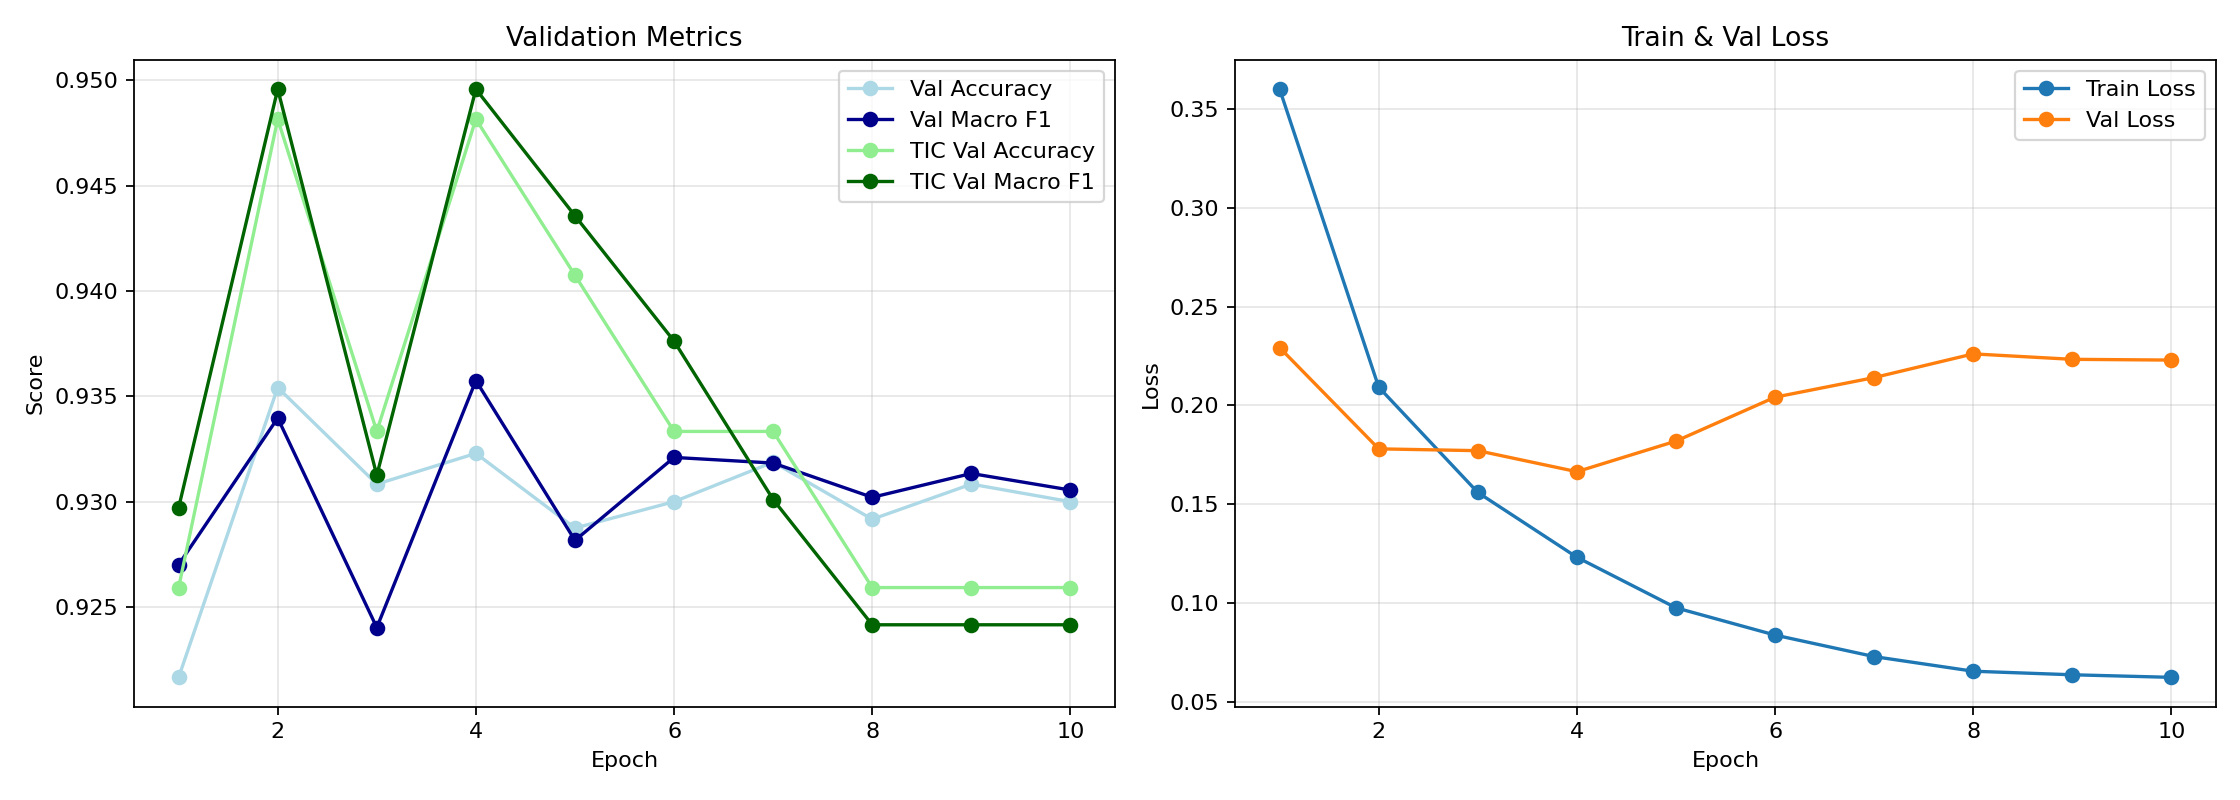
\includegraphics[width=\linewidth]{images/06/phase3_B_chronos_training_curves}
    \caption[Phase 3 -- Chronos-2 Training Curves (B)]{Chronos-2 Training Curves (Task B)}
    \label{fig:06_phase_3_chronos_training_curves_B}
\end{figure}

\FloatBarrier

Training loss again steadily decreased and quickly diverged from the validation loss, after epoch $4$ the validation performance continuously worsened.

\begin{table}[H]
    \centering
    \footnotesize
    \renewcommand{\arraystretch}{1.1}

    \begin{minipage}[t]{0.32\textwidth}
        \centering
        \begin{tabularx}{\textwidth}{X c}
            \toprule
            \textbf{Metric} & \textbf{Score} \tabularnewline
            \midrule
            Accuracy    &  0.9354 \tabularnewline
            Macro F1    & 0.9334 \tabularnewline
            TIC Accuracy & 0.9481 \tabularnewline
            TIC Macro F1 & 0.9496 \tabularnewline
            \bottomrule
        \end{tabularx}
    \end{minipage}
    \hfill
    \begin{minipage}[t]{0.64\textwidth}
        \centering
        \footnotesize
        \begin{tabularx}{\textwidth}{X c c c c c}
            \toprule
            \textbf{Class} & \textbf{Precision} & \textbf{Recall} & \textbf{F1-score} & \textbf{Support} \tabularnewline
            \midrule
            E & 0.94 & 1.00 & 0.97 & 15 \tabularnewline
            P & 0.97 & 0.94 & 0.96 & 81   \tabularnewline
            R & 0.90 & 0.95 & 0.93 & 39   \tabularnewline
            \bottomrule
        \end{tabularx}
    \end{minipage}

    \caption[Phase 3 -- Chronos-2 Validation Metrics (B)]{Chronos-2 Validation Metrics (Task B)}
    \label{tab:06_phase_3_chronos_validation_metrics_B}
\end{table}

\FloatBarrier

The Chronos-2 fine-tune again outperformed the previous best 6-channel transformer.
$\text{Val TIC Macro F1} \approx 0.95$ is a great predictive performance for a dataset of this size.

\subsection{Qwen 2.5 0.5B}

The training took around $180$ and $50$ minutes for tasks A and B respectively.

\subsubsection{Task A}

\begin{figure}[!htbp]
    \centering
    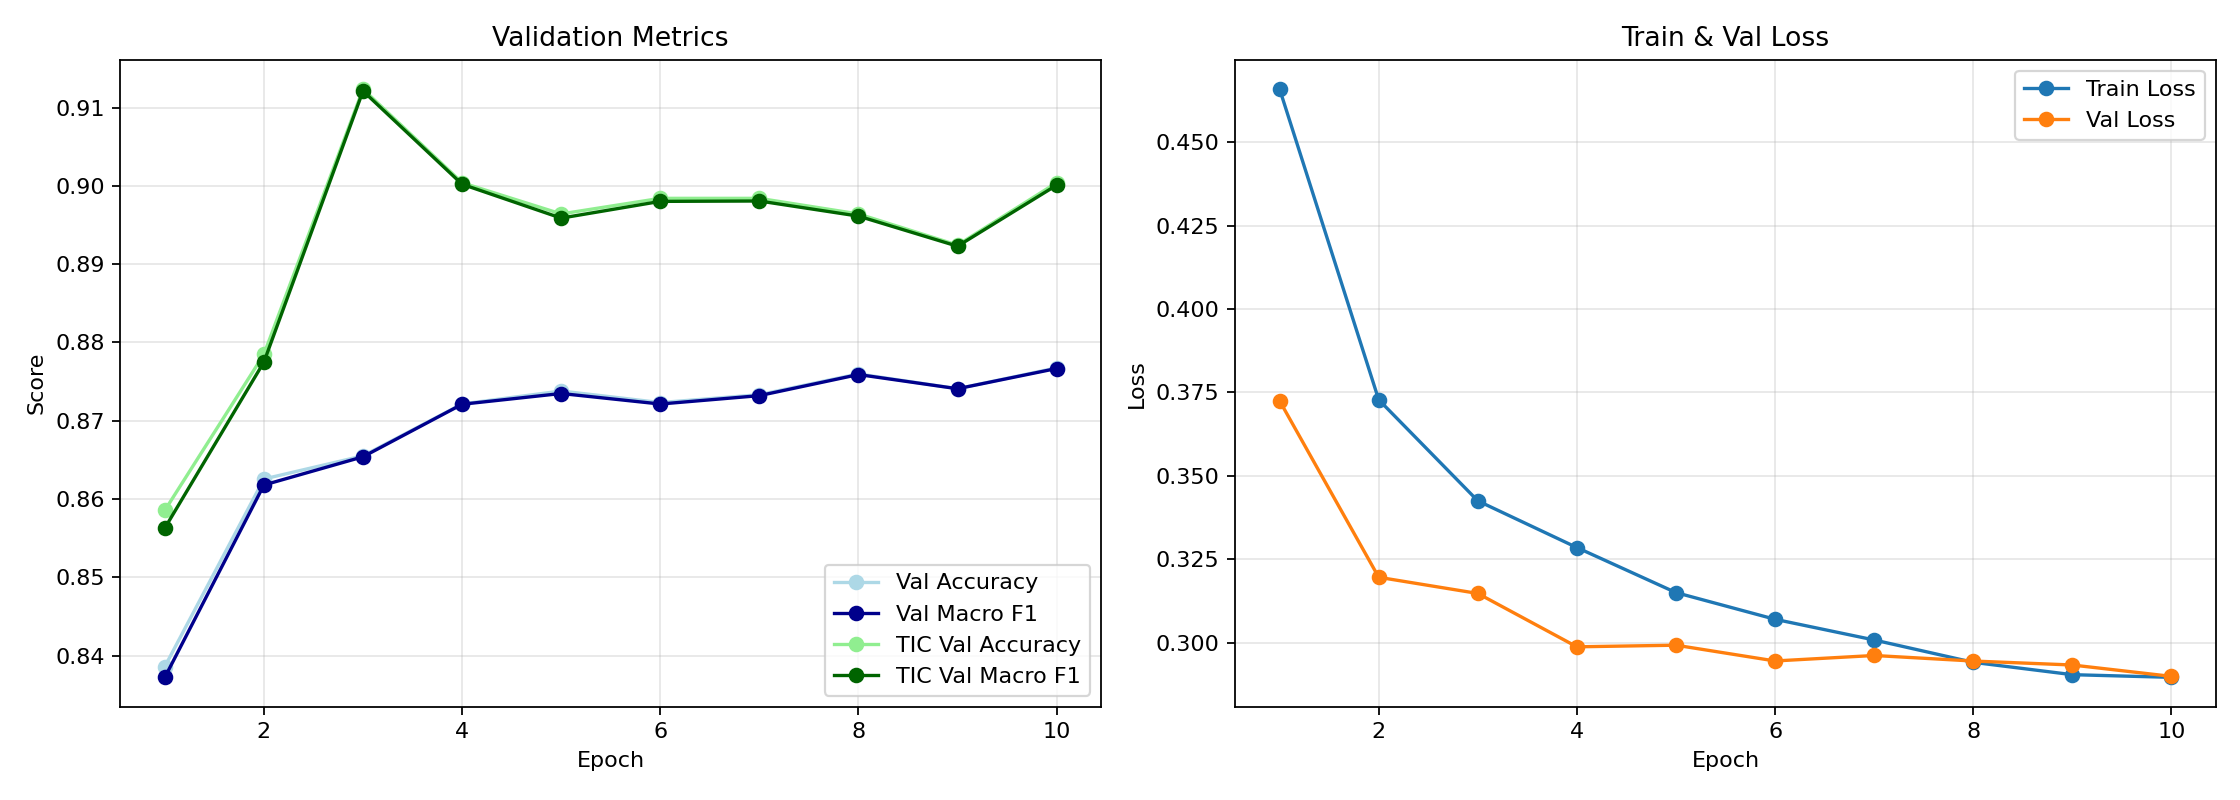
\includegraphics[width=\linewidth]{images/06/phase3_A_qwen_training_curves}
    \caption[Phase 3 -- Qwen 2.5 0.5B Training Curves (A)]{Qwen 2.5 0.5B Training Curves (Task A)}
    \label{fig:06_phase_3_qwen_training_curves_A}
\end{figure}

\FloatBarrier

\begin{table}[H]
    \centering
    \footnotesize
    \renewcommand{\arraystretch}{1.1}

    \begin{minipage}[t]{0.32\textwidth}
        \centering
        \begin{tabularx}{\textwidth}{X c}
            \toprule
            \textbf{Metric} & \textbf{Score} \tabularnewline
            \midrule
            Accuracy    &  0.8655 \tabularnewline
            Macro F1    & 0.8654 \tabularnewline
            TIC Accuracy & 0.9123 \tabularnewline
            TIC Macro F1 & 0.9121 \tabularnewline
            \bottomrule
        \end{tabularx}
    \end{minipage}
    \hfill
    \begin{minipage}[t]{0.64\textwidth}
        \centering
        \footnotesize
        \begin{tabularx}{\textwidth}{X c c c c c}
            \toprule
            \textbf{Class} & \textbf{Precision} & \textbf{Recall} & \textbf{F1-score} & \textbf{Support} \tabularnewline
            \midrule
            N & 0.90 & 0.93 & 0.92 & 259 \tabularnewline
            V & 0.93 & 0.89 & 0.91 & 243   \tabularnewline
            \bottomrule
        \end{tabularx}
    \end{minipage}

    \caption[Phase 3 -- Qwen 2.5 0.5B Validation Metrics (A)]{Qwen 2.5 0.5B Validation Metrics (Task A)}
    \label{tab:06_phase_3_qwen_validation_metrics_A}
\end{table}

\FloatBarrier

\subsubsection{Task B}

\begin{figure}[!htbp]
    \centering
    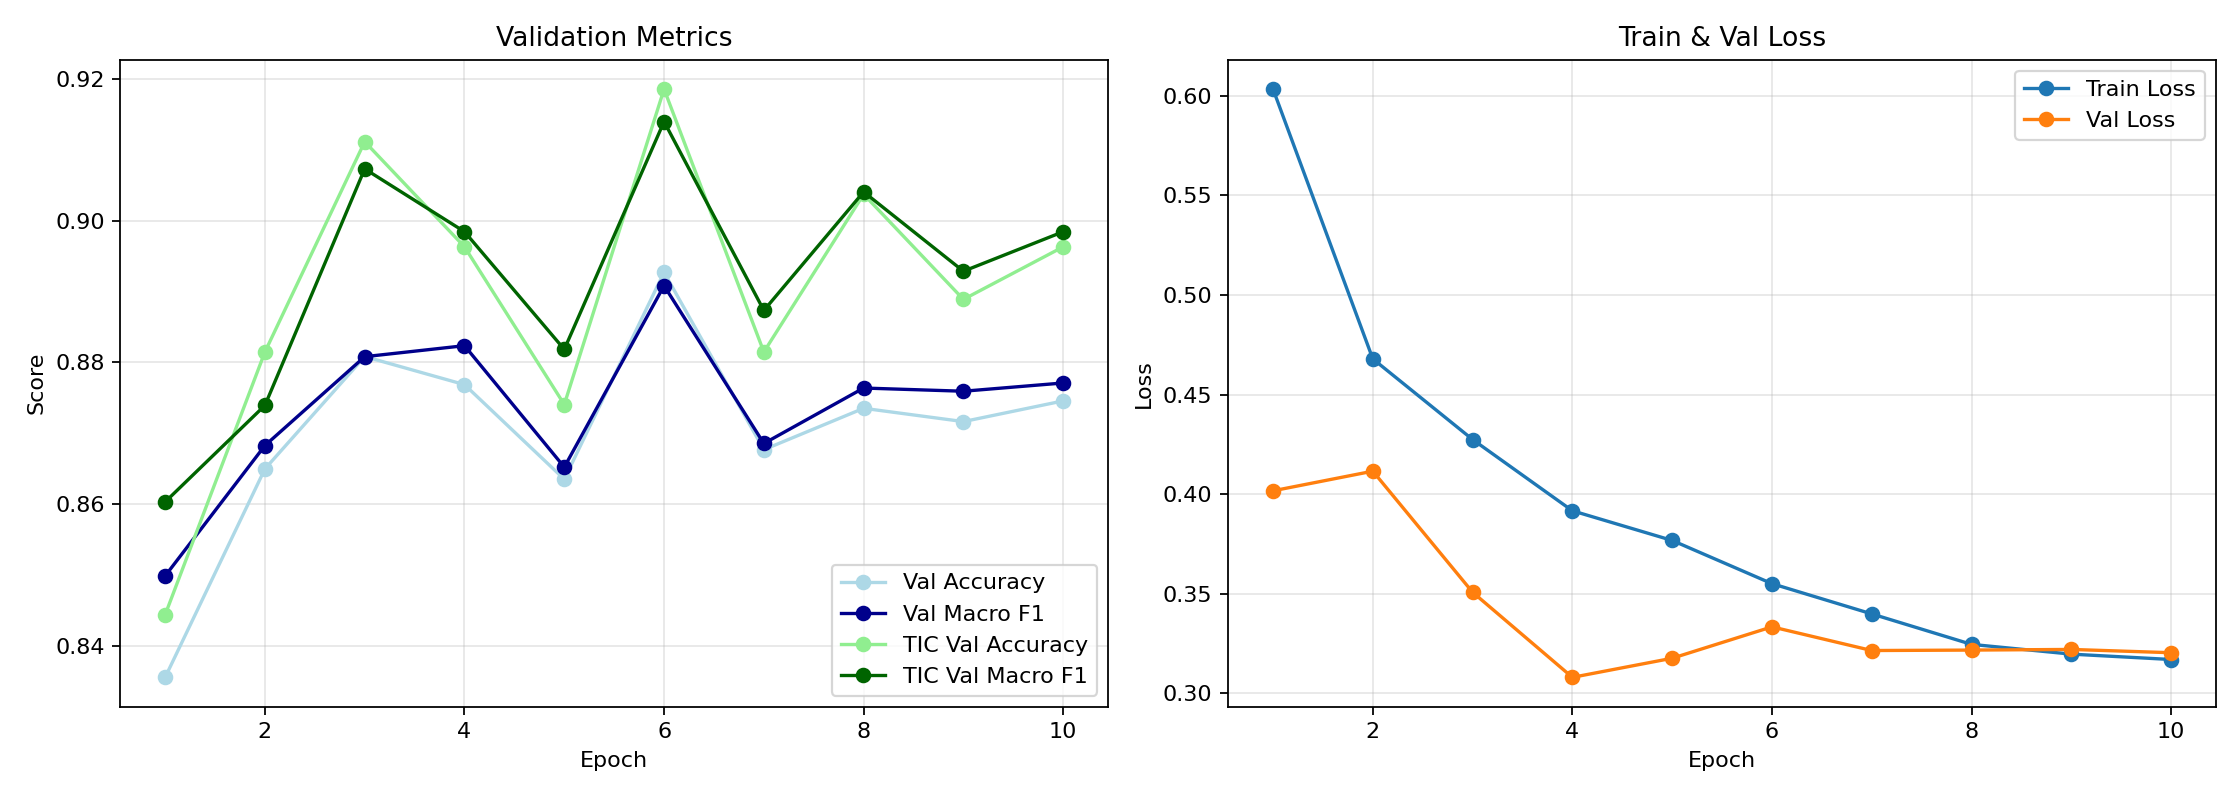
\includegraphics[width=\linewidth]{images/06/phase3_B_qwen_training_curves}
    \caption[Phase 3 -- Qwen 2.5 0.5B Training Curves (B)]{Qwen 2.5 0.5B Training Curves (Task B)}
    \label{fig:06_phase_3_qwen_training_curves_B}
\end{figure}

\FloatBarrier

\begin{table}[H]
    \centering
    \footnotesize
    \renewcommand{\arraystretch}{1.1}

    \begin{minipage}[t]{0.32\textwidth}
        \centering
        \begin{tabularx}{\textwidth}{X c}
            \toprule
            \textbf{Metric} & \textbf{Score} \tabularnewline
            \midrule
            Accuracy    &  0.8927 \tabularnewline
            Macro F1    & 0.8908 \tabularnewline
            TIC Accuracy & 0.9185 \tabularnewline
            TIC Macro F1 & 0.9139 \tabularnewline
            \bottomrule
        \end{tabularx}
    \end{minipage}
    \hfill
    \begin{minipage}[t]{0.64\textwidth}
        \centering
        \footnotesize
        \begin{tabularx}{\textwidth}{X c c c c c}
            \toprule
            \textbf{Class} & \textbf{Precision} & \textbf{Recall} & \textbf{F1-score} & \textbf{Support} \tabularnewline
            \midrule
            E & 1.00 & 0.87 & 0.93 & 15 \tabularnewline
            P & 0.94 & 0.94 & 0.94 & 81   \tabularnewline
            R & 0.85 & 0.90 & 0.88 & 39   \tabularnewline
            \bottomrule
        \end{tabularx}
    \end{minipage}

    \caption[Phase 3 --Qwen 2.5 0.5B Validation Metrics (B)]{Qwen 2.5 0.5B Validation Metrics (Task B)}
    \label{tab:06_phase_3_qwen_validation_metrics_B}
\end{table}

\FloatBarrier

While the Qwen 2.5 0.5B was underfitted and the performance could probably be improved with more epochs, it didn't generalize well enough to justify spending the extensive amounts compute required for more experiments.


\section{Experiment Summary}

We provide a summary of the $16$ experiments showcased in this work.

\begin{table}[H]
    \scriptsize
    \centering
    \renewcommand{\arraystretch}{1.3}
    \begin{tabularx}{\textwidth}{X c@{\hspace{3em}}c@{\hspace{3em}}c}
        \toprule
        \textbf{Task} & \textbf{Model} & \textbf{Architecture}  & \textbf{Val TIC Macro F1}  \tabularnewline \midrule
        \textbf{A} &
        \begin{tabular}{@{}c@{}}
            2-min \\ 8-min \\ 32-min \\ 128-min \\ 4-channel \\ 6-channel \\ \textbf{Chronos-2} \\ Qwen 2.5 0.5B
        \end{tabular} &
        \begin{tabular}{@{}c@{}}
            Transformer \\ Transformer \\ Transformer \\ Transformer \\ Transformer \\ Transformer \\ \textbf{TSFM fine-tune} \\ LLM fine-tune
        \end{tabular} &
        \begin{tabular}{@{}c@{}}
            0.8396 \\ 0.8704 \\ 0.8684 \\ 0.8436 \\ 0.8931 \\ 0.8983 \\ \textbf{0.9261} \\ 0.9129
        \end{tabular} \tabularnewline \midrule
        \textbf{B} &
        \begin{tabular}{@{}c@{}}
            2-min \\ 8-min \\ 32-min \\ 128-min \\ 4-channel \\ 6-channel \\ \textbf{Chronos-2} \\ Qwen 2.5 0.5B
        \end{tabular} &
        \begin{tabular}{@{}c@{}}
            Transformer \\ Transformer \\ Transformer \\ Transformer \\ Transformer \\ Transformer \\ \textbf{TSFM fine-tune} \\ LLM fine-tune
        \end{tabular} &
        \begin{tabular}{@{}c@{}}
            0.6618 \\ 0.8223 \\ 0.8614 \\ 0.9110 \\ 0.9230 \\ 0.9240 \\ \textbf{0.9496} \\ 0.9139
        \end{tabular} \tabularnewline
        \bottomrule
    \end{tabularx}
    \caption[Experiment]{Experiment Summary}
    \label{tab:06_experiment_summary}
\end{table}

\FloatBarrier

As can be seen from \hyperref[tab:06_experiment_summary]{Table 6.21}, the Chronos-2 fine-tunes dominated both tasks, significantly outperforming the other models.


\section{Final Model}

Since the Chronos-2 fine-tune performed the best out of all the evaluated configurations, we used it for more experiments, trying to further optimize the hyperparameters specifically for its architecture and achieve better performance.
However, none of the techniques we tried -- increasing dropout, tuning LoRA values, trying different channel combinations and modifying the fusion head -- lead to any improvement over the original experiment.

The original model proposed in \hyperref[subsubsec:06-chronos]{6.8.1 Chronos-2} was therefore chosen as the final best model.
We use the original checkpoints with the best TIC-level Macro F1 (epoch 5 for Task A and epoch 4 for task B) to evaluate the final model's performance on the test set which should simulate new, unknown data.
The model shouldn't be significantly overfitted on either of those checkpoints, since the training validation loss wasn't increasing yet and the training loss was only slightly lower.

\subsection{Task A Test Evaluation and Discussion}

\begin{table}[H]
    \centering
    \footnotesize
    \renewcommand{\arraystretch}{1.1}

    \begin{minipage}[t]{0.32\textwidth}
        \centering
        \begin{tabularx}{\textwidth}{X c}
            \toprule
            \textbf{Metric} & \textbf{Score} \tabularnewline
            \midrule
            Accuracy    &  0.8702 \tabularnewline
            Macro F1    & 0.8693 \tabularnewline
            TIC Accuracy & 0.8946 \tabularnewline
            TIC Macro F1 & 0.8934 \tabularnewline
            \bottomrule
        \end{tabularx}
    \end{minipage}
    \hfill
    \begin{minipage}[t]{0.64\textwidth}
        \centering
        \footnotesize
        \begin{tabularx}{\textwidth}{X c c c c c}
            \toprule
            \textbf{Class} & \textbf{Precision} & \textbf{Recall} & \textbf{F1-score} & \textbf{Support} \tabularnewline
            \midrule
            N & 0.85 & 0.97 & 0.90 & 259 \tabularnewline
            V & 0.96 & 0.82 & 0.88 & 243   \tabularnewline
            \bottomrule
        \end{tabularx}
    \end{minipage}

    \caption[Final Model Test Metrics (A)]{Final Model Test Metrics (Task A)}
    \label{tab:06_final_model_test_metrics_A}
\end{table}

The test TIC-level Macro F1 went down $\approx 0.02$, this can be expected and is a good generalization performance on a dataset of this size.
It should however be noted that for the \textbf{variable} class the precision increased and recall decreased significantly when compared to the validation metrics.

This behavior has interesting implications for real-world use cases -- for example, the model would be really effective in precisely identifying variable stars, that could be utilized to create large datasets consisting of (mostly) variable stars that could be later used for unsupervised pretraining.
However, the downside is that the model will miss out on some potentially interesting variable stars due to its low recall.

\subsection{Task B Test Evaluation and Discussion}

\begin{table}[H]
    \centering
    \footnotesize
    \renewcommand{\arraystretch}{1.1}

    \begin{minipage}[t]{0.32\textwidth}
        \centering
        \begin{tabularx}{\textwidth}{X c}
            \toprule
            \textbf{Metric} & \textbf{Score} \tabularnewline
            \midrule
            Accuracy    &  0.8998 \tabularnewline
            Macro F1    & 0.8340 \tabularnewline
            TIC Accuracy & 0.9333 \tabularnewline
            TIC Macro F1 & 0.8803 \tabularnewline
            \bottomrule
        \end{tabularx}
    \end{minipage}
    \hfill
    \begin{minipage}[t]{0.64\textwidth}
        \centering
        \footnotesize
        \begin{tabularx}{\textwidth}{X c c c c c}
            \toprule
            \textbf{Class} & \textbf{Precision} & \textbf{Recall} & \textbf{F1-score} & \textbf{Support} \tabularnewline
            \midrule
            E & 0.83 & 0.67 & 0.74 & 15 \tabularnewline
            P & 0.94 & 0.99 & 0.96 & 81   \tabularnewline
            R & 0.94 & 0.93 & 0.94 & 39   \tabularnewline
            \bottomrule
        \end{tabularx}
    \end{minipage}

    \caption[Final Model Test Metrics (B)]{Final Model Test Metrics (Task B)}
    \label{tab:06_final_model_test_metrics_B}
\end{table}

The TIC-level Macro F1 dropped significantly ($\Delta \approx 0.07$) compared to the validation set.
Interestingly, the entire drop in performance was caused by the misclassification of $5$ \textbf{eclipsing} stars as another class which lead to greatly decreased recall and eventually Macro F1 score.

We have investigated the 5 misclassified eclipsing stars and found out that each of them was an interesting non-standard example.

\begin{table}[H]
    \centering
    \small
    \renewcommand{\arraystretch}{1.3}
    \begin{tabularx}{\textwidth}{X c X}
        \toprule
        \textbf{TIC} & \textbf{Eclipsing Subclass} & \textbf{Note} \tabularnewline
        \midrule
        224595426 & EA & Extremely noisy, the eclipses are not easily identifiable. \tabularnewline
        229710150 & ELL & Peaks are not sharp -- similar to a rotating star. \tabularnewline
        259238257 & ELL & Peaks are not sharp -- similar to a rotating star. \tabularnewline
        288346083 & EA & Atypically long period -- the eclipse happened only once per 50 days. \tabularnewline
        362226108 & EW & Very similar to a pulsating star. \tabularnewline
        \bottomrule
    \end{tabularx}
    \caption[Missclassified Eclipsing Stars]{Misclassified Eclipsing Stars}
    \label{tab:06_misclassified_eclipsing_stars}
\end{table}

\begin{figure}[!htbp]
    \centering
    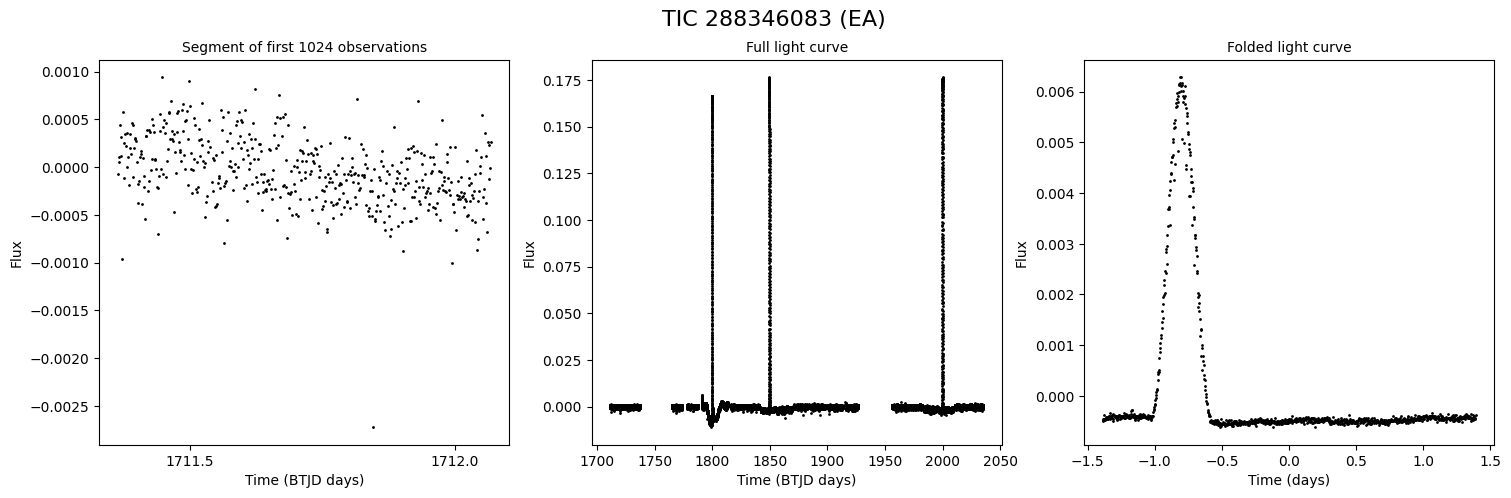
\includegraphics[width=\linewidth]{images/06/long_period_star}
    \caption[Long Period EA Star]{TIC 288346083, a misclassified eclipsing star with atypically long period.}
    \label{fig:06_long_period_star}
\end{figure}

Despite the worse performance on the \textbf{eclipsing} class, the model has generalized well on the remaining 2 classes, their test metrics being nearly identical to the validation metrics.


\section{Computational Performance}

For usage on large real-world datasets, the model must be able to efficiently process large volumes of data (millions of light curves).
We provide a brief analysis of the model's processing speed using available data.

There are 2 main possible bottlenecks:

\begin{itemize}
    \item \textbf{Preprocessing}
    \item \textbf{Inference}
\end{itemize}

\subsection{Preprocessing}

The preprocessing speed was $\approx 13.8 \, \text{light curves/s}$ on AMD Ryzen 5 9700X CPU when utilizing all 8 cores or around \num{1200000} light curves per day.
While the preprocessing pipeline could certainly be optimized, it would probably not achieve more than $10\times$ speedup.

\subsection{Inference}

Information from the training logs shows that model took $10.7$ seconds to run evaluation on the val subset of $135$ light curves, making the inference speed $\approx 12.6 \, \text{light curves/s}$ or around \num{1100000} on an AMD Radeon RX9070 GPU.

\subsection{Summary}

With the available information, we can conclude that the pipeline is theoretically capable of analyzing up to millions of light curves in reasonable time (days) on higher end consumer-grade hardware.
The processing speed could be further increased by utilizing industrial-grade GPU clusters and more parallelization.
    \chapter{Results and Discussion}

\section{Experiment Summary}

We provide a summary of the $16$ experiments showcased in this work.

\begin{table}[H]
    \scriptsize
    \centering
    \renewcommand{\arraystretch}{1.3}
    \begin{tabularx}{\textwidth}{X c@{\hspace{3em}}c@{\hspace{3em}}c}
        \toprule
        \textbf{Task} & \textbf{Model} & \textbf{Architecture}  & \textbf{Val TIC Macro F1}  \tabularnewline \midrule
        \textbf{A} &
        \begin{tabular}{@{}c@{}}
            Baseline \\ 2-min \\ 8-min \\ 32-min \\ 128-min \\ 4-channel \\ 6-channel \\ \textbf{Chronos-2} \\ Qwen 2.5 0.5B
        \end{tabular} &
        \begin{tabular}{@{}c@{}}
            CNN \\ Transformer \\ Transformer \\ Transformer \\ Transformer \\ Transformer \\ Transformer \\ \textbf{TSFM fine-tune} \\ LLM fine-tune
        \end{tabular} &
        \begin{tabular}{@{}c@{}}
            9061 \\ 0.8396 \\ 0.8704 \\ 0.8684 \\ 0.8436 \\ 0.8931 \\ 0.8983 \\ \textbf{0.9261} \\ 0.9129
        \end{tabular} \tabularnewline \midrule
        \textbf{B} &
        \begin{tabular}{@{}c@{}}
            Baseline \\ 2-min \\ 8-min \\ 32-min \\ 128-min \\ 4-channel \\ 6-channel \\ \textbf{Chronos-2} \\ Qwen 2.5 0.5B
        \end{tabular} &
        \begin{tabular}{@{}c@{}}
            CNN \\ Transformer \\ Transformer \\ Transformer \\ Transformer \\ Transformer \\ Transformer \\ \textbf{TSFM fine-tune} \\ LLM fine-tune
        \end{tabular} &
        \begin{tabular}{@{}c@{}}
            0.9232 \\ 0.6618 \\ 0.8223 \\ 0.8614 \\ 0.9110 \\ 0.9230 \\ 0.9240 \\ \textbf{0.9496} \\ 0.9139
        \end{tabular} \tabularnewline
        \bottomrule
    \end{tabularx}
    \caption[Experiment]{Experiment Summary}
    \label{tab:06_experiment_summary}
\end{table}

\FloatBarrier

As can be seen from \hyperref[tab:06_experiment_summary]{Table 7.1}, the Chronos-2 fine-tunes dominated both tasks, significantly outperforming the other models and was the only model that outperformed the baseline CNN on both tasks.

Because of the low gap between the baseline CNN and the evaluated models that had access to the same training information (all 6 channels enabled), we theorize that the majority of the performance was decided by the multi-channel architecture and light curve segmentation.
The Chronos-2 fine-tune nonetheless consistently beat the CNN which showcased the adaptability of large pretrained transformer models on our task.

\section{Final Model}

Since the Chronos-2 fine-tune performed the best out of all the evaluated configurations, we used it for more experiments, trying to further optimize the hyperparameters specifically for its architecture and achieve better performance.
However, none of the techniques we tried -- increasing dropout, tuning LoRA values, trying different channel combinations and modifying the fusion head -- lead to any improvement over the original experiment.

The original model proposed in \hyperref[subsubsec:06-chronos]{6.9.1 Chronos-2} was therefore chosen as the final best model.
We use the original checkpoints with the best TIC-level Macro F1 (epoch 5 for Task A and epoch 4 for task B) to evaluate the final model's performance on the test set which should simulate new, unknown data.
The model shouldn't be significantly overfitted on either of those checkpoints, since the training validation loss wasn't increasing yet and the training loss was only slightly lower.

\subsection{Task A Test Evaluation and Discussion}

\begin{table}[H]
    \centering
    \footnotesize
    \renewcommand{\arraystretch}{1.1}

    \begin{minipage}[t]{0.32\textwidth}
        \centering
        \begin{tabularx}{\textwidth}{X c}
            \toprule
            \textbf{Metric} & \textbf{Score} \tabularnewline
            \midrule
            Accuracy    &  0.8702 \tabularnewline
            Macro F1    & 0.8693 \tabularnewline
            TIC Accuracy & 0.8946 \tabularnewline
            TIC Macro F1 & 0.8934 \tabularnewline
            \bottomrule
        \end{tabularx}
    \end{minipage}
    \hfill
    \begin{minipage}[t]{0.64\textwidth}
        \centering
        \footnotesize
        \begin{tabularx}{\textwidth}{X c c c c c}
            \toprule
            \textbf{Class} & \textbf{Precision} & \textbf{Recall} & \textbf{F1-score} & \textbf{Support} \tabularnewline
            \midrule
            N & 0.85 & 0.97 & 0.90 & 259 \tabularnewline
            V & 0.96 & 0.82 & 0.88 & 243   \tabularnewline
            \bottomrule
        \end{tabularx}
    \end{minipage}

    \caption[Final Model Test Metrics (A)]{Final Model Test Metrics (Task A)}
    \label{tab:06_final_model_test_metrics_A}
\end{table}

The test TIC-level Macro F1 went down $\approx 0.02$, this can be expected and is a good generalization performance on a dataset of this size.
It should however be noted that for the \textbf{variable} class the precision increased and recall decreased significantly when compared to the validation metrics.

This behavior has interesting implications for real-world use cases -- for example, the model would be really effective in precisely identifying variable stars, that could be utilized to create large datasets consisting of (mostly) variable stars that could be later used for unsupervised pretraining.
However, the downside is that the model will miss out on some potentially interesting variable stars due to its low recall.

\subsection{Task B Test Evaluation and Discussion}

\begin{table}[H]
    \centering
    \footnotesize
    \renewcommand{\arraystretch}{1.1}

    \begin{minipage}[t]{0.32\textwidth}
        \centering
        \begin{tabularx}{\textwidth}{X c}
            \toprule
            \textbf{Metric} & \textbf{Score} \tabularnewline
            \midrule
            Accuracy    &  0.8998 \tabularnewline
            Macro F1    & 0.8340 \tabularnewline
            TIC Accuracy & 0.9333 \tabularnewline
            TIC Macro F1 & 0.8803 \tabularnewline
            \bottomrule
        \end{tabularx}
    \end{minipage}
    \hfill
    \begin{minipage}[t]{0.64\textwidth}
        \centering
        \footnotesize
        \begin{tabularx}{\textwidth}{X c c c c c}
            \toprule
            \textbf{Class} & \textbf{Precision} & \textbf{Recall} & \textbf{F1-score} & \textbf{Support} \tabularnewline
            \midrule
            E & 0.83 & 0.67 & 0.74 & 15 \tabularnewline
            P & 0.94 & 0.99 & 0.96 & 81   \tabularnewline
            R & 0.94 & 0.93 & 0.94 & 39   \tabularnewline
            \bottomrule
        \end{tabularx}
    \end{minipage}

    \caption[Final Model Test Metrics (B)]{Final Model Test Metrics (Task B)}
    \label{tab:06_final_model_test_metrics_B}
\end{table}

The TIC-level Macro F1 dropped significantly ($\Delta \approx 0.07$) compared to the validation set.
Interestingly, the entire drop in performance was caused by the misclassification of $5$ \textbf{eclipsing} stars as another class which lead to greatly decreased recall and eventually Macro F1 score.

We have investigated the 5 misclassified eclipsing stars and found out that each of them was an interesting non-standard example.

\begin{table}[H]
    \centering
    \small
    \renewcommand{\arraystretch}{1.3}
    \begin{tabularx}{\textwidth}{X c X}
        \toprule
        \textbf{TIC} & \textbf{Eclipsing Subclass} & \textbf{Note} \tabularnewline
        \midrule
        224595426 & EA & Extremely noisy, the eclipses are not easily identifiable. \tabularnewline
        229710150 & ELL & Peaks are not sharp -- similar to a rotating star. \tabularnewline
        259238257 & ELL & Peaks are not sharp -- similar to a rotating star. \tabularnewline
        288346083 & EA & Atypically long period -- the eclipse happened only once per 50 days. \tabularnewline
        362226108 & EW & Very similar to a pulsating star. \tabularnewline
        \bottomrule
    \end{tabularx}
    \caption[Missclassified Eclipsing Stars]{Misclassified Eclipsing Stars}
    \label{tab:06_misclassified_eclipsing_stars}
\end{table}

\FloatBarrier

\begin{figure}[!htbp]
    \centering
    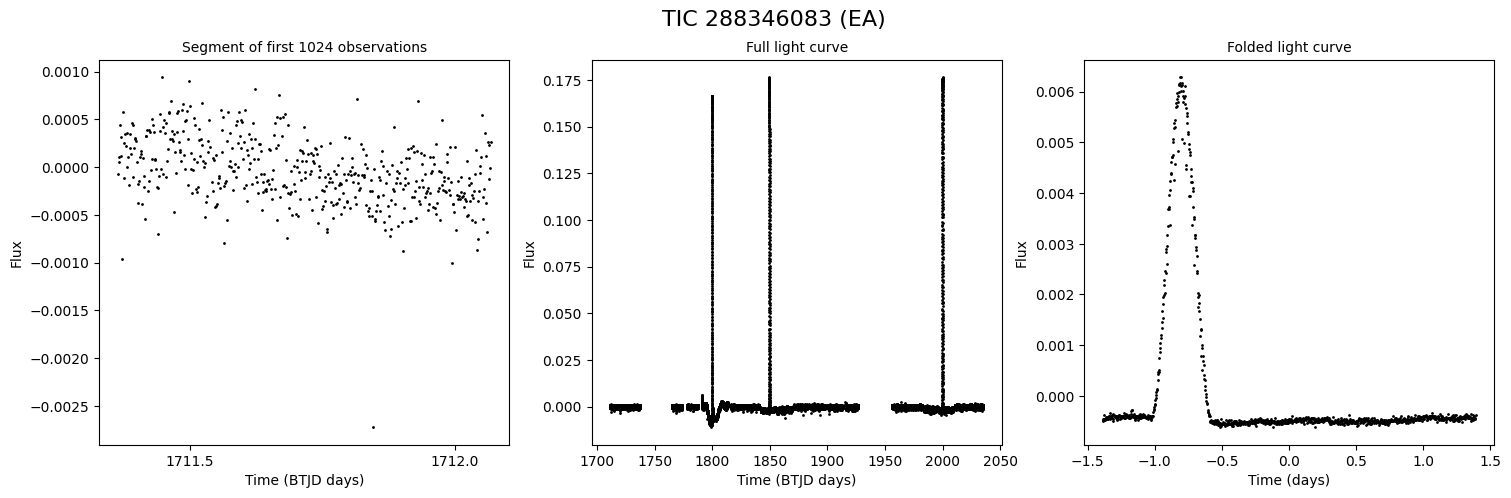
\includegraphics[width=\linewidth]{images/06/long_period_star}
    \caption[Long Period EA Star]{TIC 288346083, a misclassified eclipsing star with atypically long period.}
    \label{fig:06_long_period_star}
\end{figure}

\FloatBarrier

Despite the worse performance on the \textbf{eclipsing} class, the model has generalized well on the remaining 2 classes, their test metrics being nearly identical to the validation metrics.


\section{Computational Performance}

For usage on large real-world datasets, the model must be able to efficiently process large volumes of data (millions of light curves).
We provide a brief analysis of the model's processing speed using available data.

There are 2 main possible bottlenecks:

\begin{itemize}
    \item \textbf{Preprocessing}
    \item \textbf{Inference}
\end{itemize}

\subsection{Preprocessing}

The preprocessing speed was $\approx 13.8 \, \text{light curves/s}$ on AMD Ryzen 5 9700X CPU when utilizing all 8 cores or around \num{1200000} light curves per day.
While the preprocessing pipeline could certainly be optimized, it would probably not achieve more than $10\times$ speedup.

\subsection{Inference}

Information from the training logs shows that model took $10.7$ seconds to run evaluation on the val subset of $135$ light curves, making the inference speed $\approx 12.6 \, \text{light curves/s}$ or around \num{1100000} on an AMD Radeon RX9070 GPU.

\subsection{Summary}

With the available information, we can conclude that the pipeline is theoretically capable of analyzing up to millions of light curves in reasonable time (days) on higher end consumer-grade hardware.
The processing speed could be further increased by utilizing industrial-grade GPU clusters and more parallelization.
    \chapter{Conclusion}

In this thesis, we have explored the classification of variable stars using \linebreak transformer-based models.
Theoretical foundations concerning both the astronomical and machine learning sides were established in the initial chapters, the astronomical knowledge of the problem was later crucial for designing a~suitable representation of the data for the transformer models.

Then, a separate experiment concerning classification of ECG signals was conducted to gain practical experience with transformer-based classifiers \linebreak on~a~well-documented task -- the MIT BIH dataset.
The experiment was successful and the results were competitive when compared with both transformer and non-transformer based methods implemented by other authors on the same dataset.

For light-curve classification, we used a manually labeled dataset derived from observations from the TESS mission.
We created a robust preprocessing pipeline that extracted multiple views of different resolutions, allowing the model to capture patterns from different timescales.
Additionally, each light curve was also split into multiple segments which increased the dataset size and improved training performance.

Next, we implemented a modular model architecture that could effectively handle the input data with multiple channels.
Extensive experimentation with different model configurations was performed on both transformers trained from scratch and fine-tunes of pretrained models.
The best performing model was a fine-tune of the Chronos 2 pretrained TSFM and has shown promising results for further applications.

\section{Viability of Results}

The thesis is a part of an ongoing research by the Astronomical Institute of Czech Academy of Sciences, whose purpose is the implementation of an~automated classifier that can help identify interesting objects, especially exoplanets.

Existing pipelines for the identification of exoplanets produce large amounts of false positives, usually misclassifying a variable star as an exoplanet.
Additional filtering of these results is therefore necessary and the proposed model (Task B) could further reduce the number of false positives by correctly identifying pulsating and rotating variables (exoplanets are extremely rare and their light curves are very similar to those of eclipsing binaries).

Furthermore, two important missions regarding light curves are scheduled in the near future -- Gaia mission DR4 \parencite{Prusti2016} (new data release scheduled for December 2026) and PLATO mission \parencite{Rauer2025} (spacecraft launch scheduled for January 2027).
These missions will produce large amounts of light curves that will need to be processed and our models could either directly help the filtering or serve as a foundation for more research.

\section{Further Improvements}

Advanced model architectures like gated FFNs, FFT-based attention and hybrid fusion techniques are used in modern transformer architectures and could be utilized to improve the model's performance.
Unsupervised pretraining methods using unlabeled light curves are also a promising option that could help the model learn the general structure of the data without the need for limited labeled sets.

Furthermore, having a larger labeled dataset for training would also improve the predictive performance.


    \appendix\appendixinit % do not remove these two commands

    \backmatter % do not remove this command

    \printbibliography % print out the BibLaTeX-generated bibliography list

    \chapter{Contents of the attachment}
% Contents of the attachment

	\dirtree{%
		.1 /.
		.2 data.\DTcomment{Training Datasets}.
		.2 experiment\_results.\DTcomment{Experiment logs and results}.
		.2 src.
		.3 ecg\DTcomment{ECG experiment source codes}.
		.3 lightcurves\DTcomment{Light Curve modelling source codes}.
		.3 thesis\DTcomment{\LaTeX{} source files for the thesis text}.
		.2 text.
		.3 thesis.pdf\DTcomment{Compiled thesis PDF}.
		.2 .gitattributes.
		.2 .gitignore.
		.2 compile.sh\DTcomment{Script used for compilation of the thesis}.
		.2 index.html\DTcomment{Redirects to the thesis.pdf}.
		.2 LICENSE.
		.2 README.md\DTcomment{Summary README file}.
		.2 THIRD\_PARTY\_LICENSE.md\DTcomment{Licenses of used libraries}.
	}
 % include `medium.tex' from `text/' subdirectory

\end{document}
